\documentclass[10pt,a4j,dvipdfmx]{jarticle}
%---------------------------------------------------
\usepackage{hyperref}
\usepackage{pxjahyper}
\usepackage{bm}
\usepackage{graphicx}
\usepackage{amssymb,amsmath}
\usepackage{ascmac}
\usepackage{float}
\usepackage{setspace}
\usepackage[dvips,usenames]{color}
\usepackage{colortbl}
\usepackage{algorithm}
\usepackage{algorithmic}
\usepackage{setspace}
\usepackage{subfigure}
\usepackage{here}
\usepackage[deluxe,bold]{otf}
\usepackage[haranoaji]{pxchfon}
\usepackage{redeffont}
\usepackage{listings,jvlisting} %日本語のコメントアウトをする場合jvlisting(もしくはjlisting)が必要
\usepackage{booktabs}
\usepackage{siunitx}
\usepackage{fancybox}
%---------------------------------------------------
% \definecolor{bl}{rgb}{0.94,0.97,1}
% \definecolor{gr}{rgb}{0.5,0.5,0.5}
% \makeatletter
% \def\section{\newpage\@startsection {section}{1}{\z@}{2.3ex plus -1ex minus -.2ex}{2.3 ex plus .2ex}{\Large\bf}}
% \makeatother
%---------------------------------------------------
\setlength{\textwidth}{160truemm}
\setlength{\textheight}{240truemm}
\setlength{\topmargin}{-14.5truemm}
\setlength{\oddsidemargin}{-0.5truemm}
\setlength{\headheight}{0truemm}
\setlength{\parindent}{1zw}
\setlength{\abovedisplayskip}{-2pt} % 数式上部のマージン
\setlength{\belowdisplayskip}{-2pt} % 数式下部のマージン
%---------------------------------------------------
\setstretch{1.2}
%---------------------------------------------------
\renewcommand{\subfigtopskip}{5pt}	% 図の上の隙間。上図の副題と下図の間。
\renewcommand{\subfigbottomskip}{0pt} % 図の下の隙間。副題と本題の間。
\renewcommand{\subfigcapskip}{-6pt}	% 図と副題の間
\renewcommand{\subcapsize}{\scriptsize} % 副題の文字の大きさ
\newcommand{\mysection}[1]{\vspace{-20pt}\section{#1}}
\newcommand{\mysubsection}[1]{\vspace{-20pt}\subsection{#1}}
\newcommand{\mysubsubsection}[1]{\vspace{-10pt}\subsubsection{#1}}
\renewcommand{\lstlistingname}{ソースコード}
\newcommand{\tsuyo}[1]{\textbf{\textgt{#1}}}
%---------------------------------------------------
% ヘッダーとフッターの設定
\usepackage{fancyhdr}
\rhead{ME2208 \CID{8705}橋 尚太郎}
\chead{}
\lhead{メカトロニクス レポート課題}
\cfoot{\thepage}

\rfoot{}
\begin{document}
%---------------------------------------------------
\setlength{\abovedisplayskip}{1.5pt} 
\setlength{\belowdisplayskip}{0pt}
%---------------------------------------------------
%ここからソースコードの表示に関する設定
\lstset{
  basicstyle={\ttfamily},
  identifierstyle={\small},
  commentstyle={\smallitshape},
  keywordstyle={\small\bfseries},
  ndkeywordstyle={\small},
  stringstyle={\small\ttfamily},
  frame={tb},
  breaklines=true,
  columns=[l]{fullflexible},
  numbers=left,
  xrightmargin=0zw,
  xleftmargin=3zw,
  numberstyle={\scriptsize},
  stepnumber=1,
  numbersep=1zw,
  lineskip=-0.5ex
}
%ここまでソースコードの表示に関する設定
%---------------------------------------------------

\thispagestyle{empty}
\begin{spacing}{1}

\begin{center}
\Large 明石工業高等専門学校専攻科\\[6.0truecm]
\huge \tsuyo{メカトロニクス レポート課題} \\
% \LARGE Digital Ociloscope and Waveform Processing\\
[4truecm]
\Large 報告者 \\[0.5truecm]
\Large ME2208 \CID{8705}橋 尚太郎 \\
(機械・電子システム工学専攻2年) \\[1truecm]
提出年月日:\today
\end{center}

% \begin{center}
% \vspace*{3.5cm}
% {\Huge トランジスタ回路の設計}\\
% \vspace*{12.5cm}
% {\Large 電気情報工学科4年後期}\\
% {\Large 電気電子工学実験II}\\
% \vspace*{1cm}
% \end{center}

\end{spacing}
\clearpage
\pagenumbering{arabic}
\pagestyle{fancy}
\setlength{\headheight}{5truemm}

\mysection{目的}
第5章の内燃機関の性能評価に関する項目を実際に実験して確かめる。
\mysection{原理}
\subsection{空気理論サイクル}
ガソリンエンジンに代表される火花点火式のピストンエンジンサイクルは\tsuyo{オットーサイクル(Otto cycle)}と呼ばれ、
その$p$-$V$線図は図\ref{im1}に示される。
4サイクルエンジンの場合、図\ref{im1}の過程$0 \rightarrow 1$において、ガスの吸気が行われ、($P_1, T_1$)がガスの初期状態となる。
過程$1 \rightarrow 2$において、断熱圧縮を行い、過程$2 \rightarrow 3$において爆発的な燃焼が行われ、系は熱源から$Q_1$の熱量を受け取り、
最高圧力、最高温度 ($P_3, T_3$)となる。過程$3 \rightarrow 4$において、断熱膨張が行われ、外部に対して仕事を行う。
過程$4 \rightarrow 1$で放熱し、その後の状態は$(P_1, T_4)$となる。過程$1 \rightarrow 0$でガスの排気を行い、過程$0 \rightarrow 1$の吸入過程と
打ち消し合う。過程$2 \rightarrow 3$のように、容積一定のもとで加熱が行われるので、オットーサイクルは\tsuyo{等容サイクル(constant volume cycle)}とも呼ばれる。\cite{netsu}
\begin{figure}[h]
  \begin{center}
  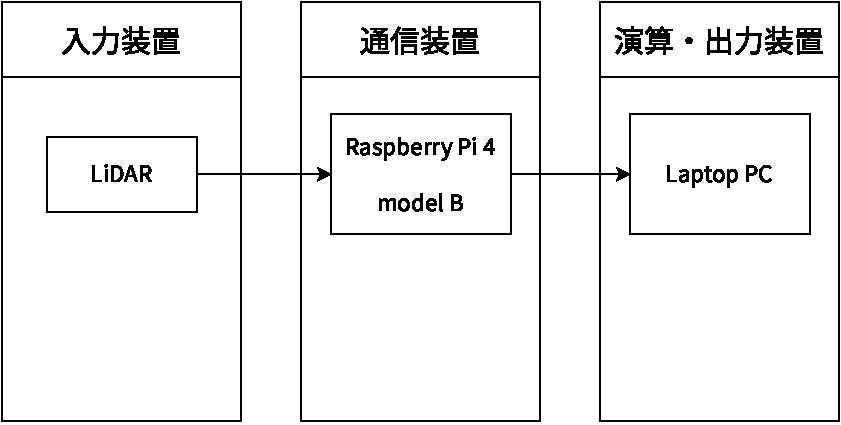
\includegraphics[width=.8\columnwidth]{img/1.pdf}
  \caption{オットーサイクルの$p$-$v$線図\cite{shiryo}}
  \label{im1}
  \end{center}
\end{figure}
以上のように、空気理論サイクルでは2つの断熱変化と2つの等容変化で構成されており、このサイクルの\tsuyo{理論熱効率(theoretical thermal efficiency)}を$\eta_{th}$とすると次式で表される。
$$\eta_{th} = \frac{Q_1-Q_2}{Q_1}\times 100 = 1-\frac{Q_2}{Q_1} \times 100 = 1-\frac{T_4-T_1}{T_3-T_2} \times 100 = 1-\frac{1}{\varepsilon^{\kappa-1}} \times 100 \si{[\%]}$$

\mysubsection{エンジン性能指標と熱勘定}
\begin{description}
  \setlength{\parskip}{0cm} % 段落間
  \setlength{\itemsep}{0cm} % 項目間
  \item[軸トルク] 回転する軸が出力できる力のこと。単位は\si{[\newton\meter]}。
  \item[軸出力] エンジンの動力取り出し軸における出力のこと。単位は\si{[\kW]}。
  \item[燃料消費率] エンジンの軸出力1\si{[\kW]}あたり1\si{[\hour]}ごとに消費される燃料の質量\si{[\g]}のこと。単
  位は\si{[\g/\kWh]}。
  \item[正味熱効率] 燃料の発熱量に対する軸出力の割合のこと。単位は\si{[\%]}。
  \item[熱勘定] 熱機関の入熱と出熱との熱平衡精算の結果である熱収支を表す方法として、
  燃料の完全燃焼により発生する熱量を100\si{\%}とし、転換したエネルギーが各部にどのように分配されているかを表すこと。
  図示仕事から運動部分の摩擦、補機類の駆動仕事を差引いて実際に機関主軸から取出せる出力を仕事に換算した\tsuyo{正味仕事}、\tsuyo{冷却損失}、\tsuyo{排気損失}および\tsuyo{機械損失}の4項目に分ける。\cite{kanjo}
\end{description}
\mysubsection{特性値の算出}
\tsuyo{特性値で用いる記号}\\
$W$:動力系制動荷重\si{[\newton]}、$N$:動力系回転数\si{[rpm]}、$T_e$:エンジン軸トルク\si{[\newton \meter]}、$P_e$:エンジン軸出力\si{[\kW]}、\\
$b$:測定時間内の燃料消費量\si{[\mL]}、$p_{me}$:正味平均有向圧\si{[\kPa]}、$V_s$:行程容積\si{[\L]}、
$a$:サイクル数/2(4サイクル:$a=2$、2サイクル:$a=1$)、$t$:燃料消費量の測定に要した時間\si{[\sec]}、$\gamma$:燃料密度\si{[0.72 \g/\mL]}、$H_l$:燃料の低位発熱量\si{[46000\kJ/\kg]}、$b_e$:燃料消費率\si{[\g/\kWh]}、$\eta_e$:正味熱効率\si{[\%]}
\begin{description}
  \setlength{\parskip}{0cm} % 段落間
  \setlength{\itemsep}{0cm} % 項目間
  \item[軸トルク] $$T_e = 0.2865 \cdot W \si{[\newton\meter]}$$
  \item[軸出力] $$P_e = \frac{W\cdot N}{33330} \si{[\kW]}$$
  \item[正味平均有向圧] $$p_{me} = \frac{60\times P_e \cdot a}{V_s\cdot N} \times 1000 \si{[\kPa]}$$
  \item[燃料消費率] $$b_e = \frac{\gamma \cdot (b/t)}{P_e} \times 3600 \si{[\g/\kWh]}$$
  \item[正味熱効率] $$\eta_e = \frac{P_e}{{\gamma\cdot (b/t)}\cdot H_l}\times 100 \si{[\%]}$$
  \item[燃料全熱量] $$Q_f = H_l\frac{\gamma(b/t)}{1000} \si{[\kW]}$$
  \item[排気損失] $$\eta_g = \frac{Q_g}{Q_f} \si{[\%]}$$
  \begin{description}
    \setlength{\parskip}{0cm} % 段落間
    \setlength{\itemsep}{0cm} % 項目間
    \item[排気損失熱量] $$Q_g = G_g c_{pg}(\si{TG1}-\si{TA1}) \si{[\kW]}$$
    \item[排気ガス流量] $$G_g = 0.072\sqrt{p_1-p_2}+\frac{\gamma(b/t)}{1000} \si{[\kg/\s]}$$
    \item[差圧] $$p_1 - p_2 = \si{DPA1} \si{[\kPa]}$$
    \item[排気ガス比熱] $$c_{pg}=1.24 \si{[\kJ/(\kg\K)]}$$
    \item[排気ガス温度] $$\si{TG1} \si{[\degreeCelsius]}$$
    \item[吸入空気温度] $$\si{TA1} \si{[\degreeCelsius]}$$
  \end{description}
  \item[冷却損失] $$\eta_w = \frac{Q_w}{Q_f}\times 100 \si{[\%]}$$
  \begin{description}
    \setlength{\parskip}{0cm} % 段落間
    \setlength{\itemsep}{0cm} % 項目間
    \item[冷却損失熱量] $$Q_w = \frac{\si{FW1}}{3600}c_{pw}(\si{TW2}-\si{TW1}) \si{[\kW]}$$
    \item[冷却水流量] $$\si{FW1} \si{[\litre/\hour]}$$
    \item[水の比熱] $$c_{pw} = 4.2 \si{[\kJ/(\kg\K)]}$$
    \item[冷却水出口温度] $$\si{TW2} \si{[\degreeCelsius]}$$
    \item[冷却水入口温度] $$\si{TW1} \si{[\degreeCelsius]}$$
  \end{description}
  \item[機械損失] $$\eta_m = 100 - (\eta_e + \eta_g + \eta_w) \si{[\%]}$$
\end{description}

\mysection{実験方法}
実験装置は、東京メーター製:内燃機関性能総合試験装置 (GWE-88/150R)であり、以下のように乗用車用エンジンと測定器で構成されている。
\begin{description}
  \setlength{\parskip}{0cm} % 段落間
  \setlength{\itemsep}{0cm} % 項目間
  \item[試験エンジン] 名称:2NZ-FE ガソリンエンジン(トヨタ自動車製)、形式:4サイクル4気筒水冷式\\総排気量:1298\si{[cc]}、圧縮比:10.5、最大軸出力:65\si{[\kW]}(6000\si{[rpm]})、最大軸トルク:121\si{[\newton\meter]}(4000\si{[rpm]}) 
  \item [測定器] 絞り弁開閉度計、動力計(腕長さ\tsuyo{286.5\si{[\milli\meter]}})、回転数計、吸入空気差圧計、燃料消費計、面積流量計、温度指示計
  \item [使用燃料] ガソリン、密度:\tsuyo{0.72\si{[\kg/\l]}}、低位発熱量\tsuyo{46000\si{[\kJ/\kg]}}
\end{description}
\mysubsection{回転数変化試験}
絞り弁開度を20\%に固定し、回転数を1600、3200、4800 \si{[rpm]}とした。指示器の計測値が安定したとき、下記項目について測定した。
\begin{description}
  \item[測定項目] 絞り弁開度、動力計制動荷重、動力計回転数、燃料消費時間、吸入空気差圧、
  吸入空気温度、\\排気ガス温度、冷却水流量、冷却水入口温度、冷却水出口温度 
\end{description}

\mysection{結果}
測定結果を表\ref{tb1}、測定結果のプロットを図\ref{plot1}~\ref{plot3}に示す。
に示す。DPA1の測定値に関して、測定値が1の位から小数第2位まで測定できる装置で、
実際の測定値が0.05、0.16、0.22であったため、小数第1位と小数第2位の数値が有効であるとする。
本実験では有効数字を3桁で示す。
$t$に関して、実際の測定値は、10の位から小数第2位の4桁であった。人間が反応するための時間は、
おおよそ0.2\si{[s]}である。これは測定値の0.5\% ~ 1\% の誤差に相当する。
本実験での計算結果に関する人間の測定による誤差の影響は、有効桁の4桁目に現れるため、
人間による時間測定の誤差は無視できるものとして扱い、本実験の数値で$t$の計算結果は有効数字2~3桁とする。

\vspace{-5truemm}
\begin{table}[h]
\centering
\caption{測定結果}
\scalebox{.8}{
\begin{tabular}[t]{crrrrrrrrrr}
\toprule
&THK\si{[\%]}&$N$\si{[rpm]}&$W$\si{[\newton]}&$t$\si{[\s]}&DPA1\si{[\kPa]}&TA1\si{[\degreeCelsius]}&TG1\si{[\degreeCelsius]}&FW1\si{[\l/\hour]}&TW1\si{[\degreeCelsius]}&TW2\si{[\degreeCelsius]}\\
\midrule
実験1&20&1600&314&53.9&0.05&25.4&674&400&22.3&51.0\\
実験2&20&3200&278&30.4&0.16&26.2&756&740&22.3&48.0\\
実験3&20&4800&200&25.8&0.22&27.6&791&785&21.9&52.0\\
\bottomrule
\label{tb1}
\end{tabular}}
\end{table}%

\vspace{-5truemm}
\begin{figure}[h]
  \begin{center}
  \subfigure[測定結果のプロット1]{
  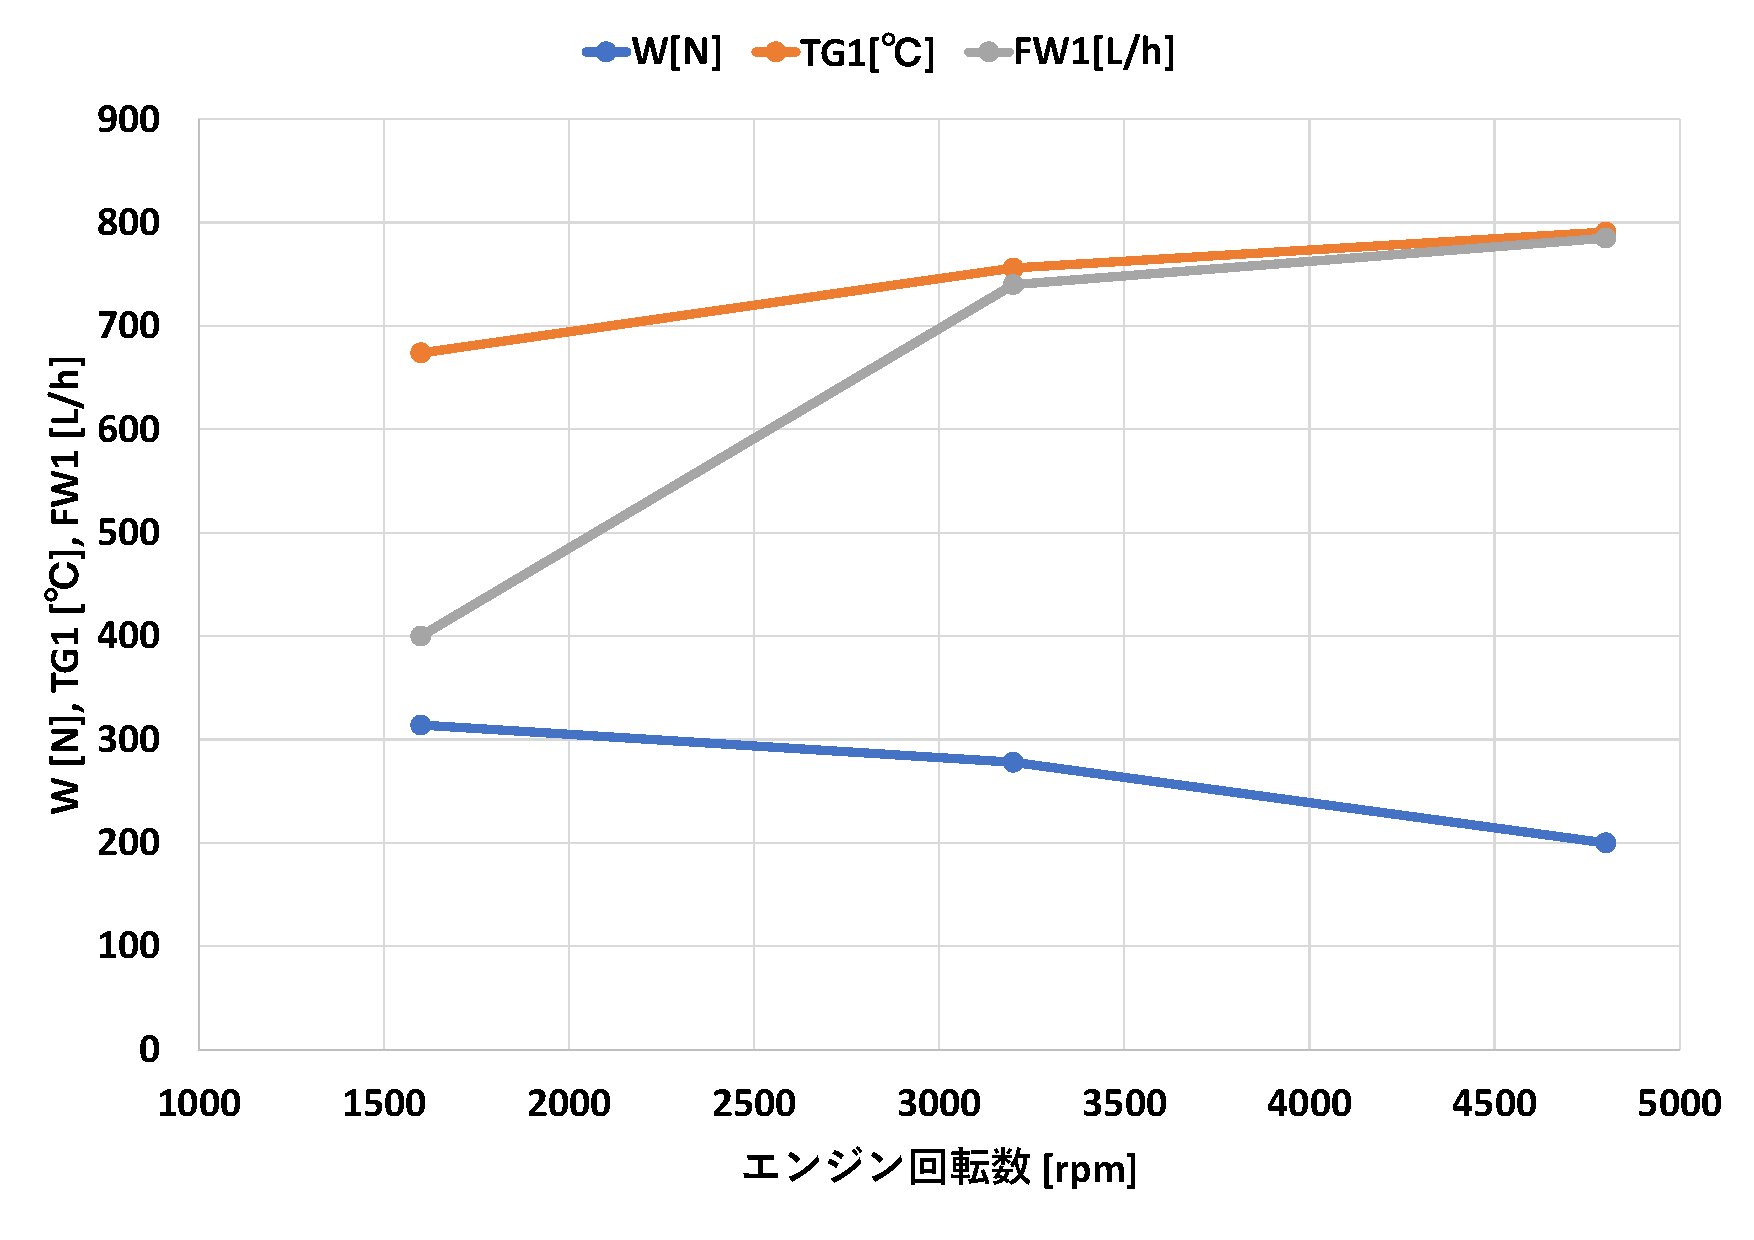
\includegraphics[width=.37\columnwidth]{img/plot1.pdf}
  \label{plot1}
  }
  \subfigure[測定結果のプロット2]{
  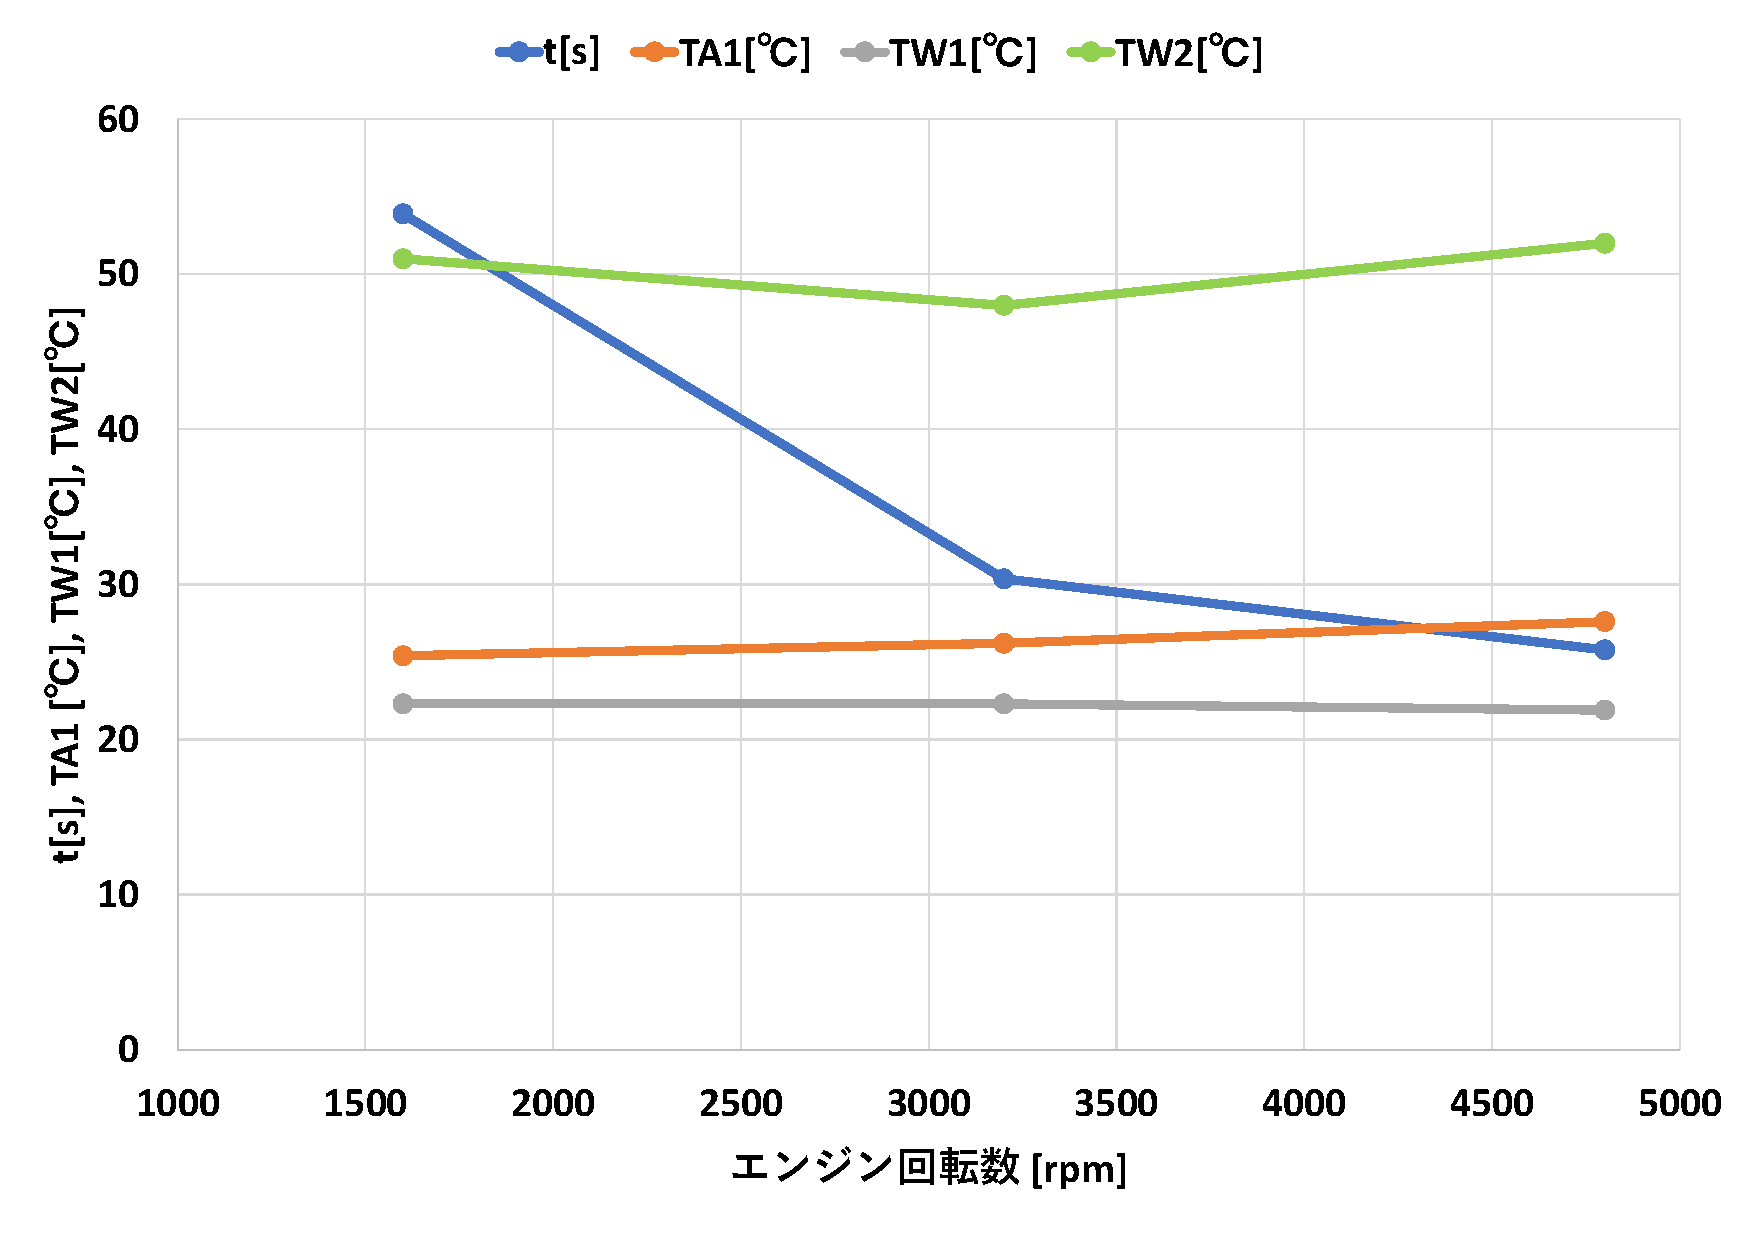
\includegraphics[width=.37\columnwidth]{img/plot2.pdf}
  \label{plot2}
  }
  \subfigure[測定結果のプロット3]{
  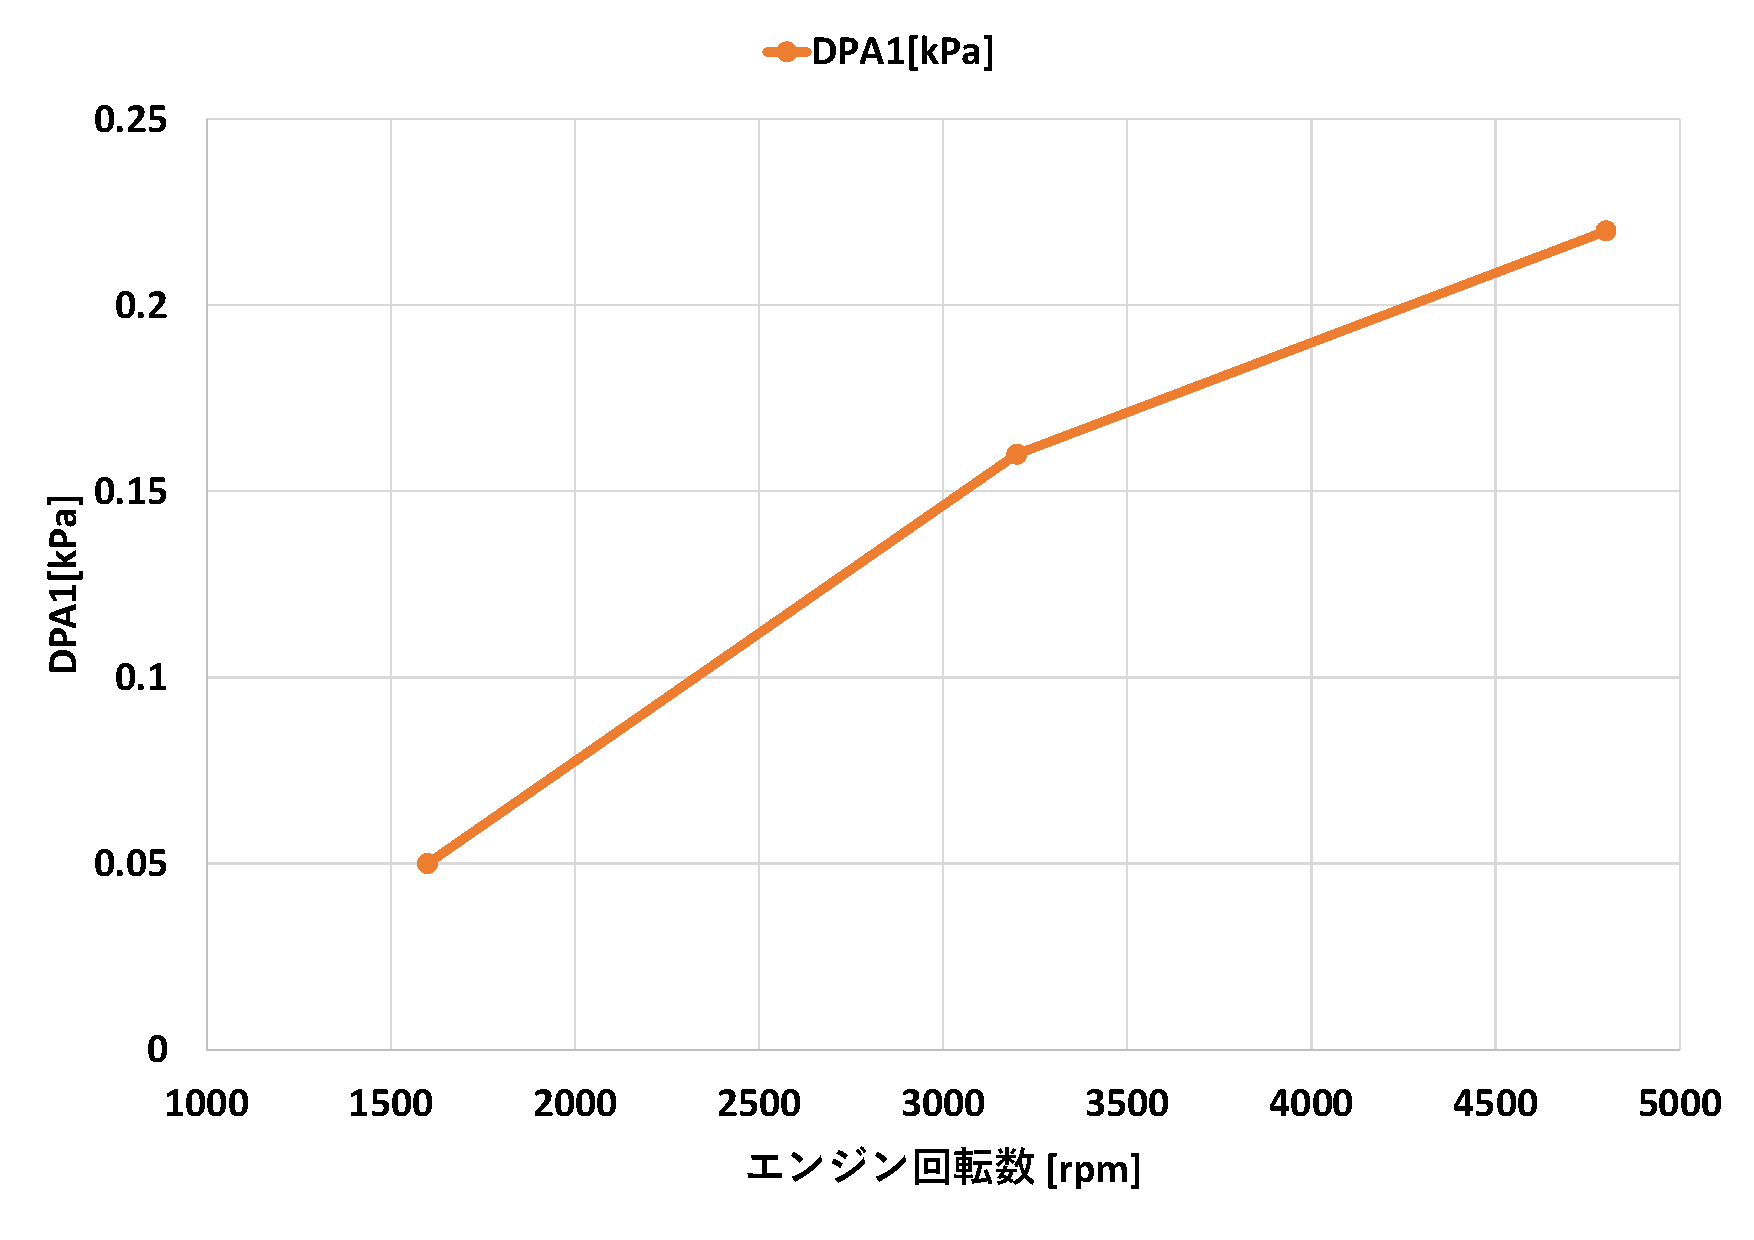
\includegraphics[width=.37\columnwidth]{img/plot3.pdf}
  \label{plot3}
  }
  \caption{測定結果のプロット}
  \end{center}
\end{figure}
\label{plot}

\mysubsection{結果の解析}
測定結果を解析することで得た特性値を表\ref{tb2}に示す。
表中の括弧内の値は図示熱効率に置き換えて算出した値である。
本実験での計算結果の有効数字は、効率は2桁、それ以外は3桁となる。

\begin{table}[h]
  \centering
  \caption{特性値}
  \scalebox{.7}{
  \begin{tabular}[t]{crrrrrrrrrrrr}
  \toprule
  &$N$\si{[rpm]}&$T_e$\si{[\newton\meter]}&$P_e$\si{[\kW]}&$b_e$\si{[\g/\kWh]}&$Q_f$\si{[\kW]}&$\eta_e$\si{[\%]}(※図示熱効率)&$G_g$\si{[\kg/\s]}&$Q_g$\si{[\kW]}&$\eta_g$\si{[\%]}&$Q_w$\si{[\kW]}&$\eta_w$\si{[\%]}&$\eta_m$\si{[\%]}\\
  \midrule
  実験1&1600&90.0&15.1&255&49.2&31 (36)&0.0172&13.8&28&13.4&27&14 (9.2)\\
  実験2&3200&80.0&31.6&256&87.2&31 (36)&0.0307&27.8&31&22.2&25&12 (6.5)\\
  実験3&4800&57.3&28.8&273&103&28 (39)&0.0360&34.1&33&27.6&27&12 (0.75)\\
  \bottomrule
  \label{tb2}
  \end{tabular}}
\end{table}%
$p$-$v$線図を図\ref{pv}、エンジン性能曲線を図\ref{engine}、
熱勘定図を図\ref{shoumi}、図\ref{zushi}に示す。

\begin{figure}[h]
  \begin{center}
  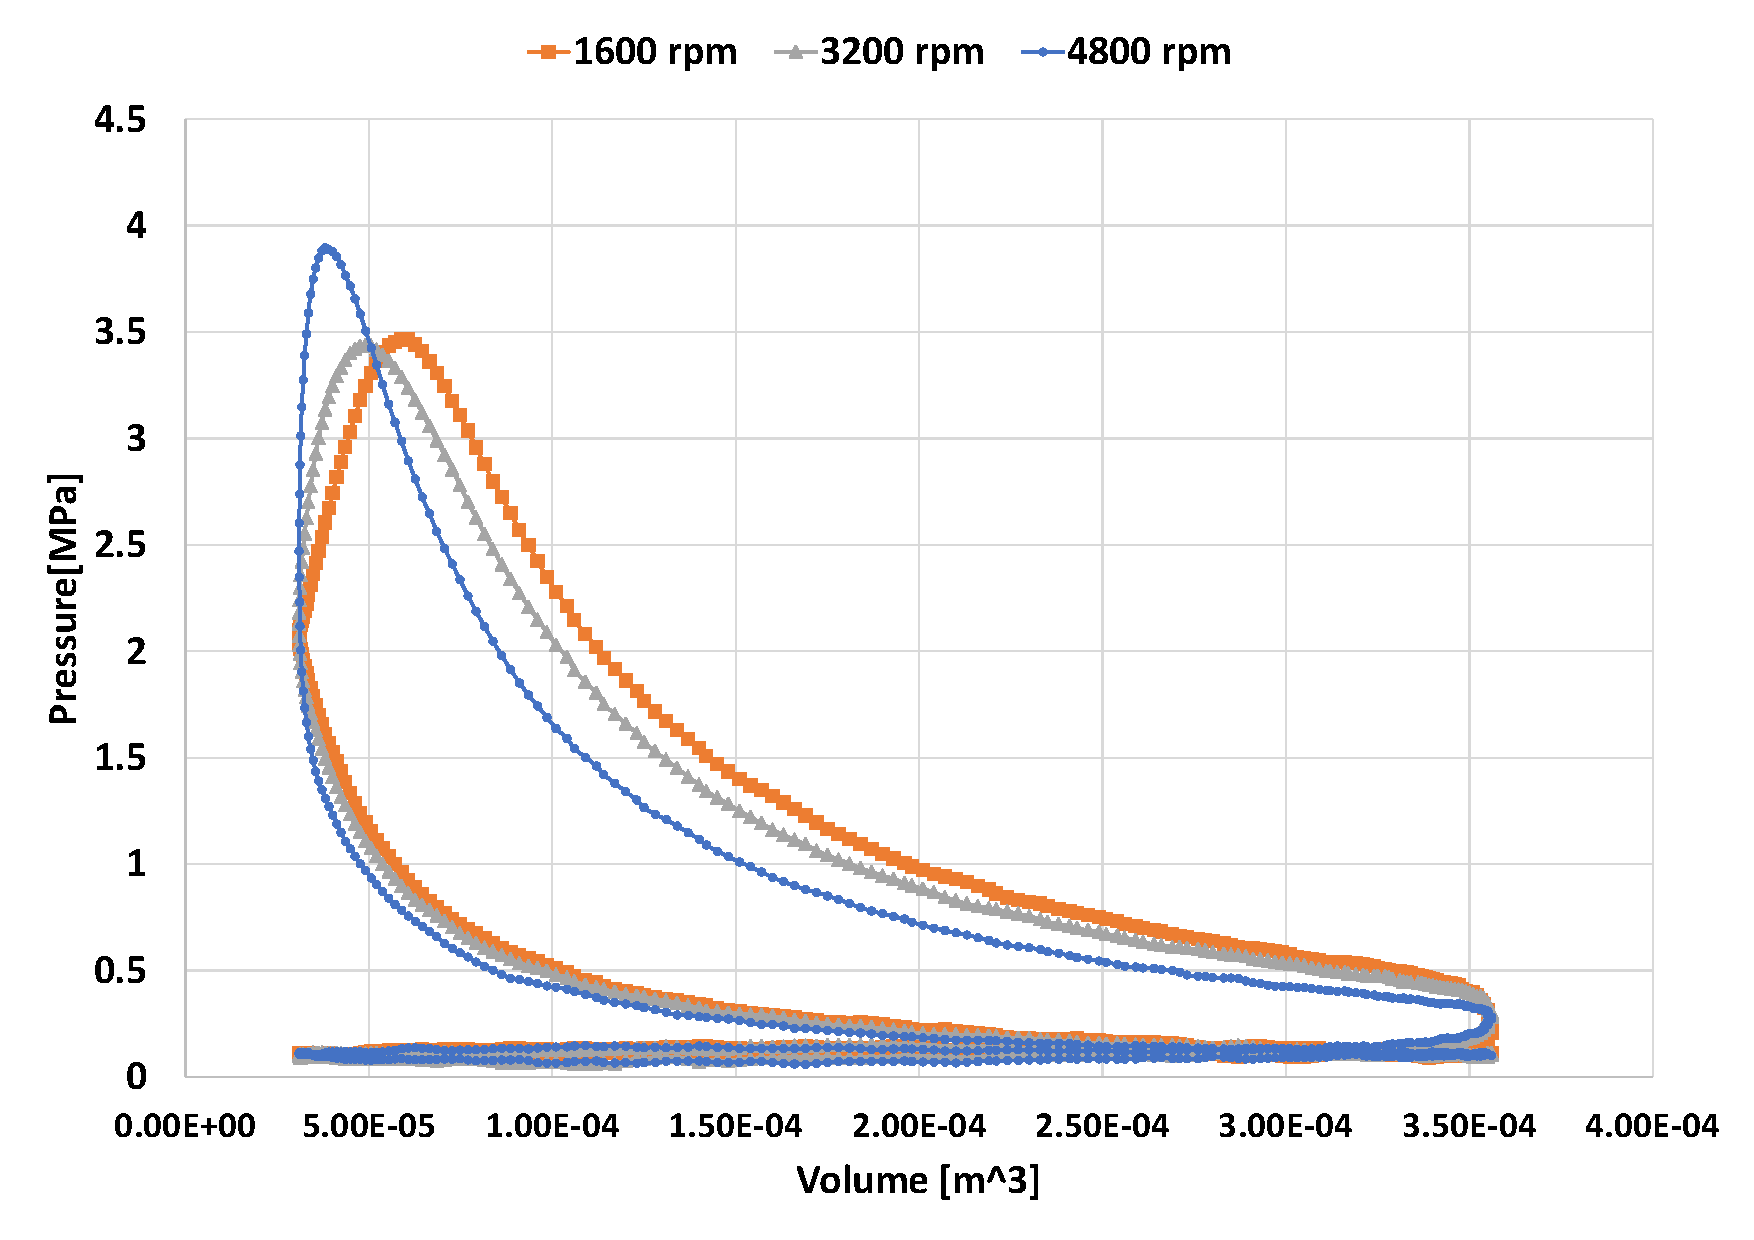
\includegraphics[width=\linewidth]{img/pv_all.pdf}
  \caption{$p$-$v$線図}
  \label{pv}
\end{center}
\end{figure}

\begin{figure}[h]
  \begin{center}
  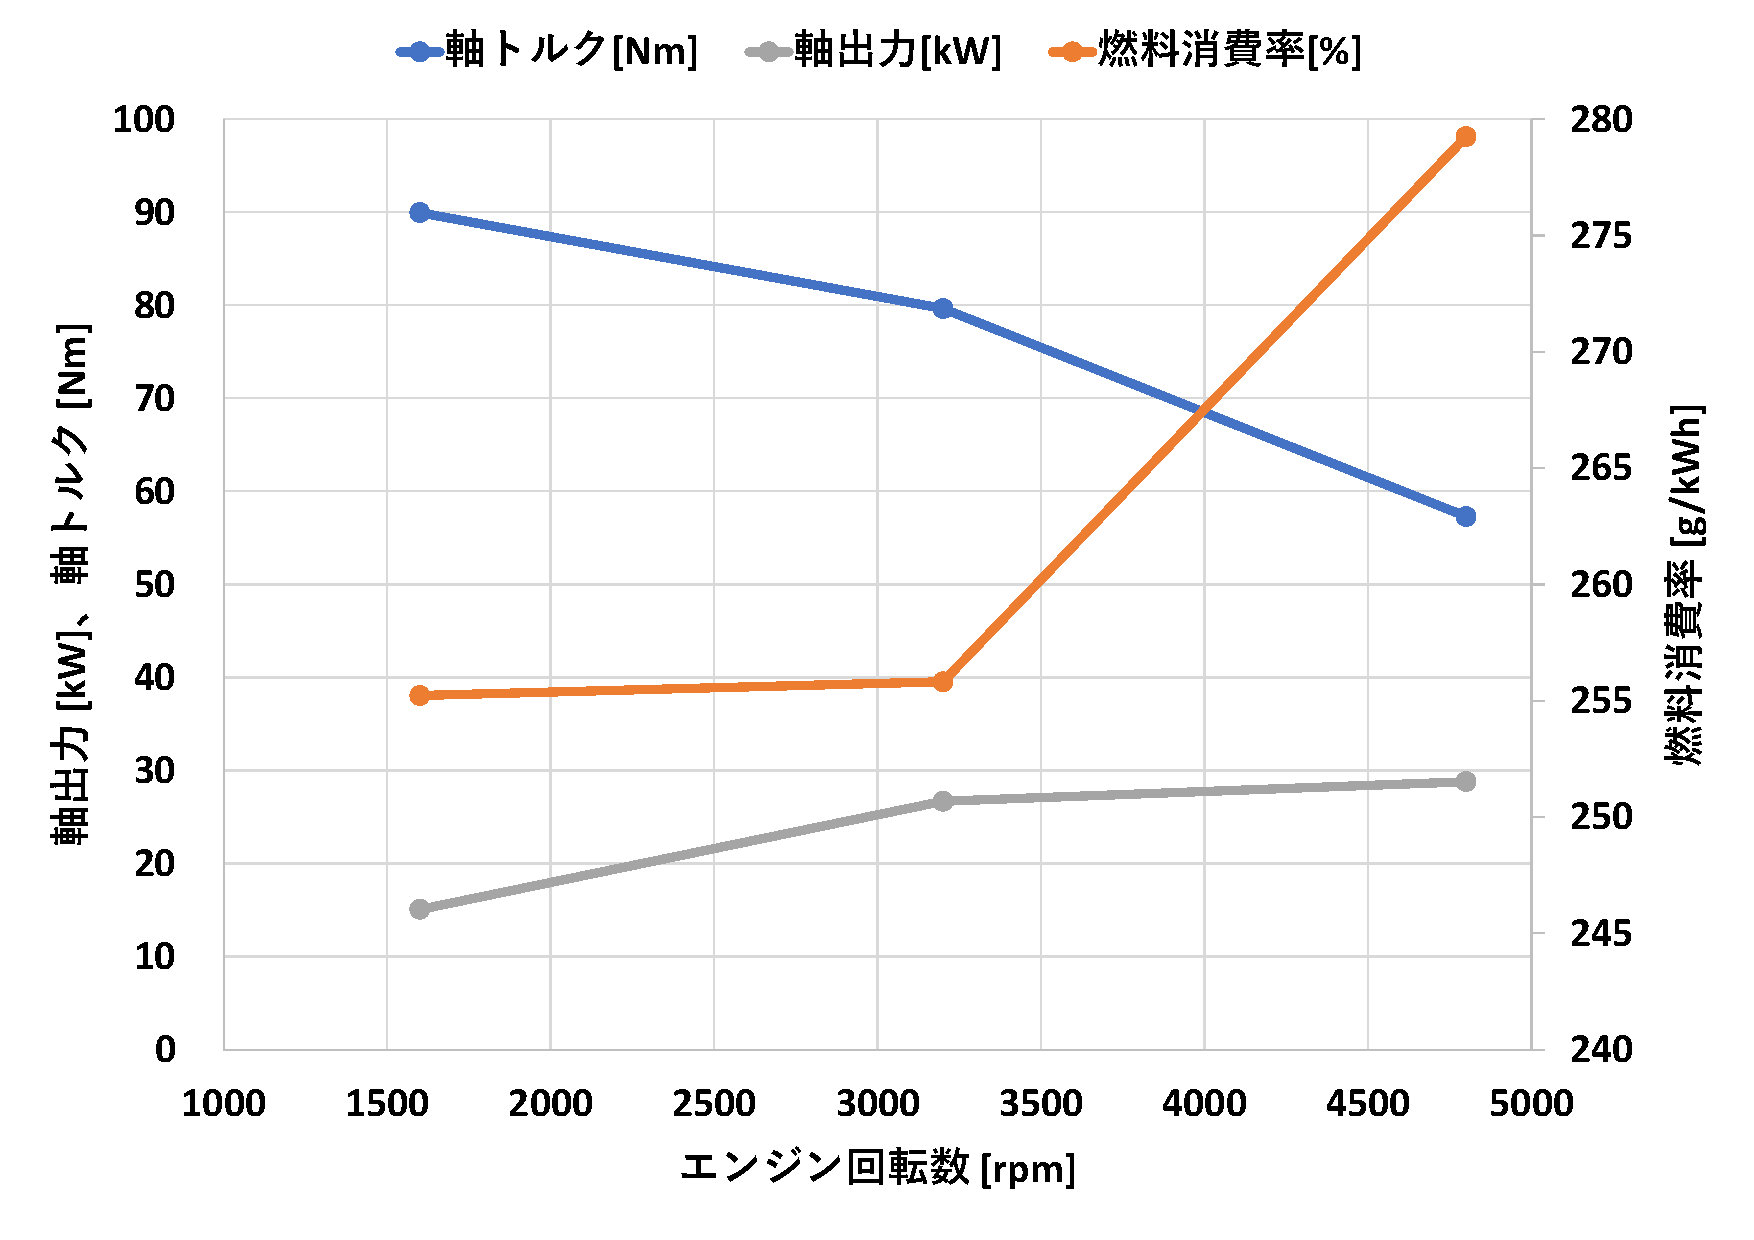
\includegraphics[width=\linewidth]{img/engine_performance.pdf}
  \caption{エンジン性能曲線}
  \label{engine}
  \end{center}
\end{figure}

\begin{figure}[h]
  \begin{center}
  \subfigure[正味熱効率を用いた場合]{
  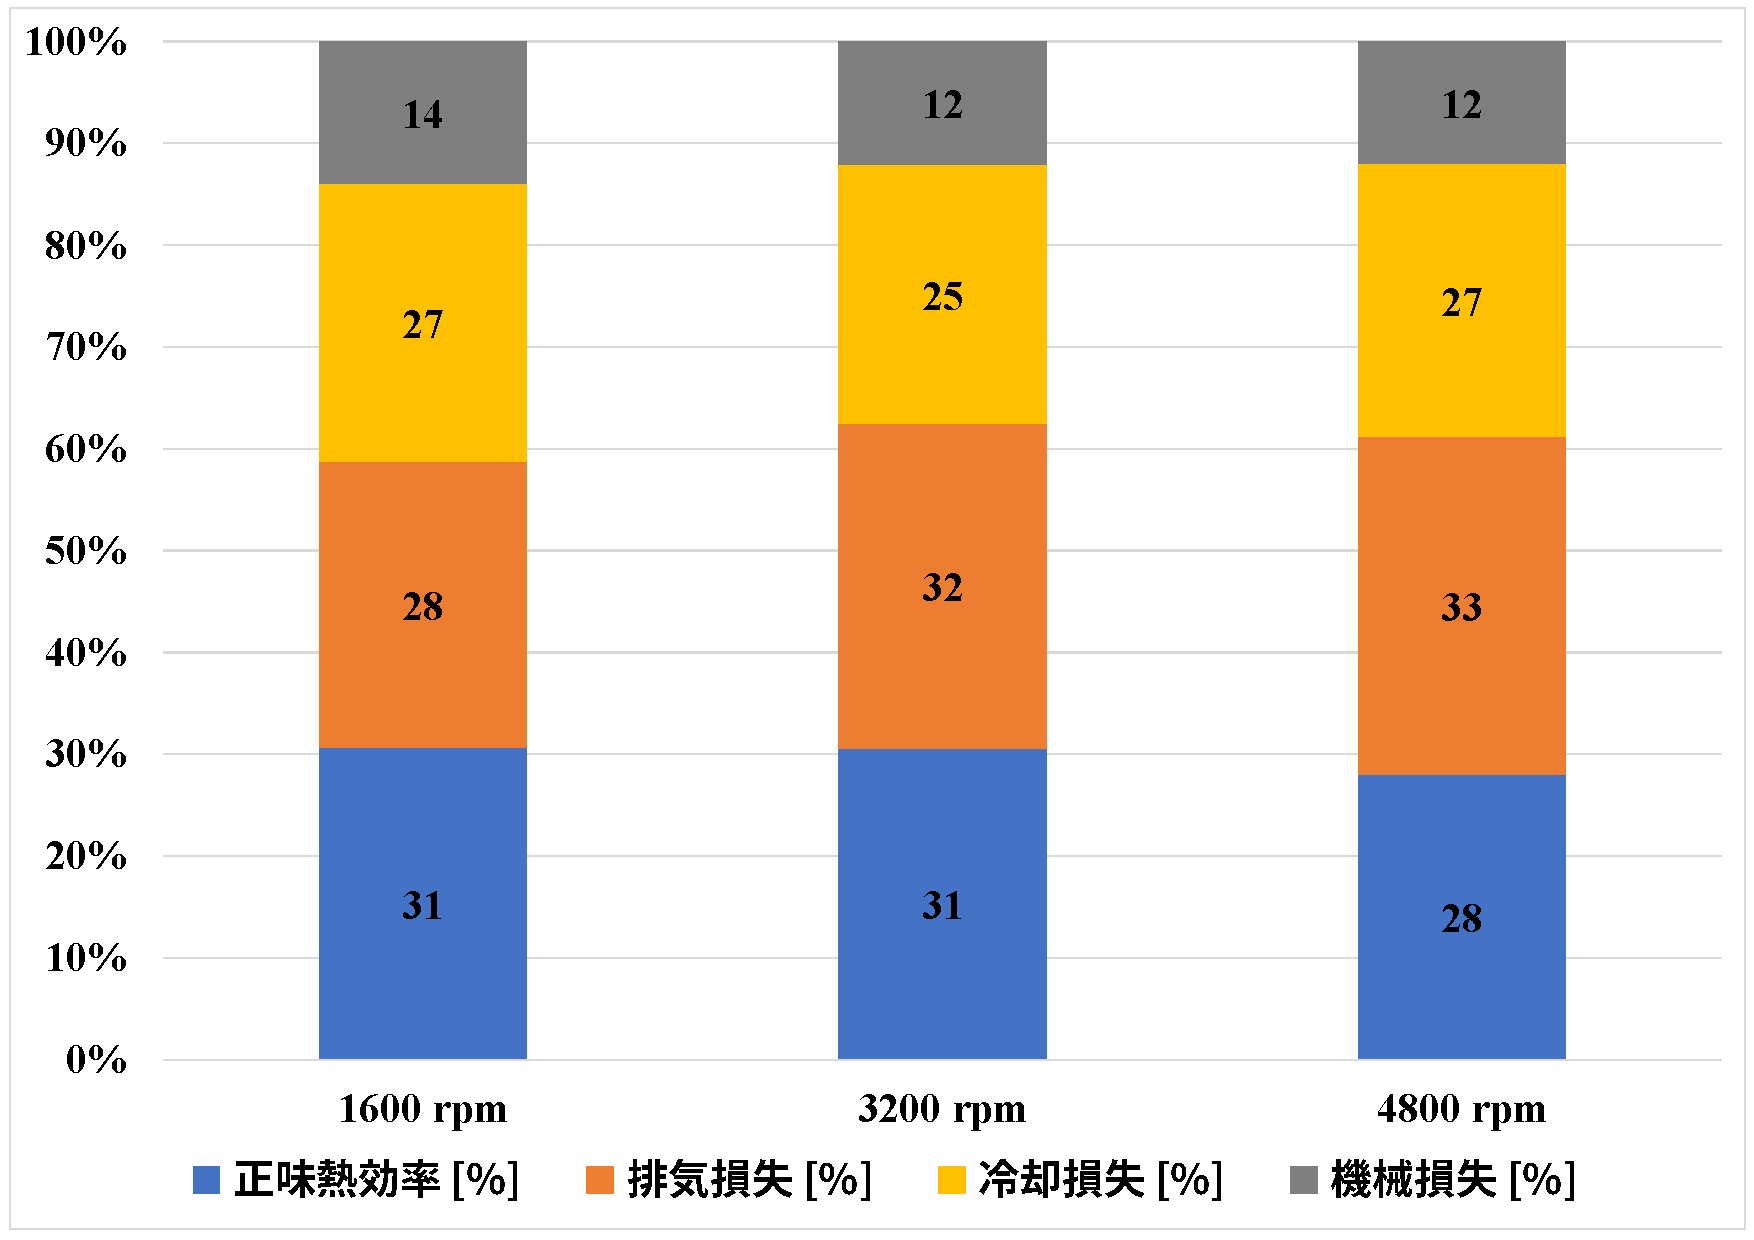
\includegraphics[width=.48\columnwidth]{img/shoumi.pdf}
  \label{shoumi}
  }
  \subfigure[図示熱効率を用いた場合]{
  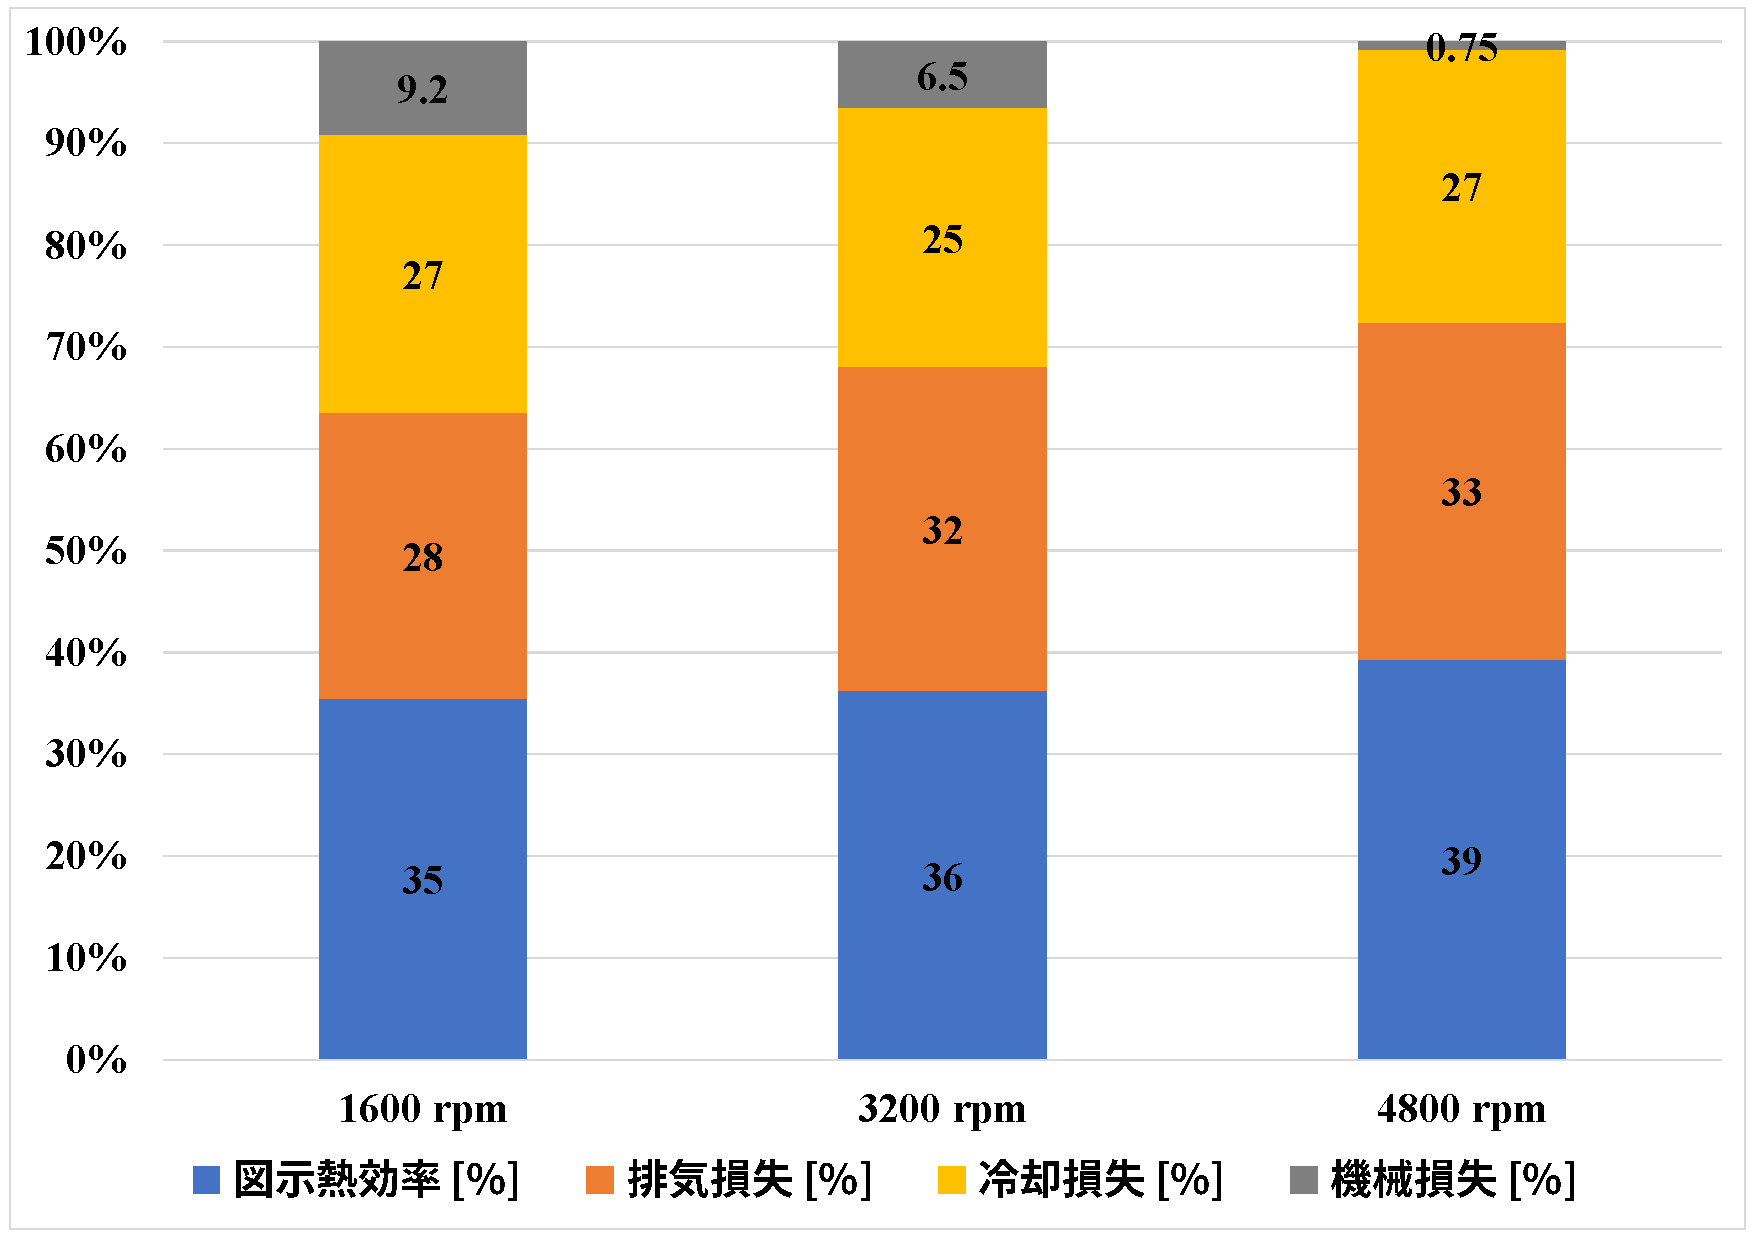
\includegraphics[width=.48\columnwidth]{img/zushi.pdf}
  \label{zushi}
  }
  \caption{熱勘定図}
  \end{center}
\end{figure}
\label{kanjou}

\clearpage

\mysection{考察}
実験結果より、冷却損失はほとんど一定であるが、排気損失がエンジンの回転数の上昇に伴ってやや増加する傾向にある。
$p$-$v$線図に関して、エンジンの回転数が4800\si{[rpm]}の際に、2$\rightarrow$3の過程において、
3における圧力が最も高く、最も直線的な形状であった。この過程は爆発的な燃焼が行われる。
表\ref{tb2}より、4800 \si{[rpm]}の際に、燃料全熱量の値が最も大きな値であったことから、
エンジンへの供給熱量が増加したためだと考えられる。また、圧力が最も高い値をとったため、
4800 \si{[rpm]} が最も熱効率が良いエンジン回転数であると考えられる。

今回実験に使用したエンジンの仕様から理論熱効率$\eta_{th}$を算出すると、式\eqref{eq1}のようになる。
\begin{equation}
  \eta_{th} = 1-\frac{1}{\varepsilon^{\kappa-1}}=1-\frac{1}{10.5^{(1.4-1)}}\fallingdotseq 0.61
  \label{eq1}
\end{equation}
つまり$\eta_{th}=\tsuyo{61\si{[\%]}}$である。


実験結果より、正味熱効率は28~30\%の値となるため、空気理論サイクルにおける理論熱効率に算出された熱(60\si{[\%]})の約半分が軸出力以外に使われたことを示している。
これらの熱は、エンジンの回転数の増加に伴い、エンジンで大きな音が生じたことや、冷却水の温度上昇、燃料消費率の上昇に伴う排気の増加(ガス交換による損失も含める)によって、
エンジン内の部品同士の摩擦による機械損失、冷却損失、排気損失に変換されたと考えられる。

また、図示熱効率はエンジンの回転数と図示出力に伴って増加する。冷却損失、排気損失は一定の
ため機械損失が減少する。しかし、実際は、エンジン内の部品の摩擦が生じるため、
機械損失がパラメータとなり、正味熱効率が減少する。よって、熱勘定図における図示熱効率と正味熱効率の偏差は、
機械損失の増加に起因すると考えられる。


これらから、\tsuyo{エンジンの高効率化}を図るために考えられることをいくつか提案する。
1つ目に\tsuyo{機械損失}を減少させるために、エンジンの熱で気化しない潤滑材を使用し、\tsuyo{摩擦を軽減する}、
2つ目に、\tsuyo{排気損失}を減少させるために、\tsuyo{燃料密度と低位発熱量がより小さい燃料}に変える、
3つ目に、\tsuyo{冷却損失}を減少させるために、\tsuyo{比熱が大きな流体を冷却に用いる}等が考えられる。

\mysection{感想}
熱機関のエネルギー効率を考える際に、理論値と実験値の考え方を区別して考えるという感覚が機械独特のものだと感じた。
理論熱効率は全てが理想的な状態と仮定した値であり、図示効率は実際に機械を動かしたものを理論に当てはめて、どんな\tsuyo{入力}があったか
を計算したもので理論と実験の中間的な値となり、正味熱効率は、機械によって実際に\tsuyo{出力}された値である。
実際に変換されているエネルギーを算出するために考慮すべき点が、電気系と比べて多く(冷却・排気・摩擦等)複雑だと感じた。
電気系は、電気そのものを得るまでに発生した損失を全て排除してから考えるから効率が高いのかもしれないと感じた。
\mysection{演習3}
\subsection{実行プログラム}
実行プログラムをソースコード\ref{s4}に示す。
\begin{lstlisting}[caption=演習3のプログラム,label=s4]
#include <stdio.h>
#include <dos.h>
#include "v25.h"
#include "ms.h"
 
int main(){
  pokeb( _V25BASE, _PMC2, 0x00 ); /*P20-P27 ポートモード*/
  pokeb( _V25BASE, _PM2, 0x00 );  /*P20-P27 出力ポート  */

  while(1){
      ms_led2( 0xff ); /* 全LEDの点灯 */
      ms_wait( 1000 ); /* 待ち時間 1s */
      ms_led2( 0x00 ); /* 全LEDの消灯 */
      ms_wait( 1000 ); /* 待ち時間 1s */
    }
  return 0;
}
\end{lstlisting}

\mysubsection{実行結果}
ポート2のLEDが点滅する。

\mysection{演習4}
\subsection{実行プログラム}
実行プログラムをソースコード\ref{s5}に示す。
\begin{lstlisting}[caption=演習4のプログラム,label=s5]
int main(){
  pokeb( _V25BASE, _PMC2, 0x00 ); /*P20-P27 ポートモード*/
  pokeb( _V25BASE, _PM2, 0x00 );  /*P20-P27 出力モード*/
 
  while(1){
    int i;
    int a = 0x01;
    for(i=0;i<8;i++)
    {
      ms_led2(a);
      ms_wait(1000);
      a = a << 1;
    }
  }
  return 0;
}
\end{lstlisting}

\subsection{実行結果}
LED0からLED7の順に点灯した後、この一連の動作を繰り返す。

\mysection{演習5}
\subsection{実行プログラム}
実行プログラムをソースコード\ref{s6}に示す。
\begin{lstlisting}[caption=演習5のプログラム,label=s6]
#include <stdio.h>
#include <dos.h>
#include "v25.h"
#include "ms.h"
  
int main(){
    int i;

    pokeb( _V25BASE, _PMC1, 0x20 ); /* P15:TOUT 出力*/
    for( i=0; i<3; i++){
        ms_beep( 440, 500 ); /* 440Hz, 0.5s */
        ms_wait( 500 ); /* 待ち時間 0.5s*/
    }
    ms_beep( 880, 1000 );
    return 0;
}
\end{lstlisting}

\mysubsection{実行結果}
440Hzの音が0.5秒毎に3回鳴った後、880Hzの音が1秒間鳴る。

\mysection{演習6}
\subsection{実行プログラム}
実行プログラムをソースコード\ref{s7}に示す。
\begin{lstlisting}[caption=演習6のプログラム,label=s7]
#include <stdio.h>
#include <dos.h>
#include "v25.h"
#include "ms.h"
  
int main(){
  int i;
  int f;
  int ms;

  pokeb( _V25BASE, _PMC1, 0x20 );
  while(1){
    scanf("%d %d", &f, &ms);
    ms_beep( f, ms ); /* 440Hz, 0.5s */
  }
  return 0;
}
\end{lstlisting}

\mysubsection{実行結果}
JTWのプロンプト上でキーボードから周波数\si{[Hz]}(スペース)時間\si{[s]}を入力して、
エンターキーを入力すると、指定した数値に応じた音がブザーから鳴る。
\mysection{演習7}
\subsection{実行プログラム}
実行プログラムをソースコード\ref{s8}に示す。

\begin{lstlisting}[caption=演習7のプログラム,label=s8]
#include <stdio.h>
#include <dos.h>
#include "v25.h"
#include "ms.h"
  
int main()
{
  int s[3];
 
  pokeb(_V25BASE, _PMC0, 0x00); 
  pokeb(_V25BASE, _PM0, 0xff);  
 
  pokeb(_V25BASE, _PMC1, 0x20); 
      
  pokeb(_V25BASE, _PMC2, 0x00); 
  pokeb(_V25BASE, _PM2, 0xff); 
  
  printf("%c[2J", 0x1b); 
  while (1){
    ms_ifr(s); 
    printf("%c[01;01H", 0x1b); 
    printf("L:%d C:%d R:%d\n", s[0], s[1], s[2]); 
  }
  return 0;
}
\end{lstlisting}

\mysubsection{実行結果}
左右と真ん中に取り付けられた3つの近接センサの値(0か1)が出力される。

\mysection{演習8}
\subsection{実行プログラム}
実行プログラムは演習7と同様である。

\subsection{実行結果}
赤外線センサの2次元的な範囲を図\ref{niji}に示す。
扇型の外側が0の値を示す。(検知範囲外である。)
斜線部と白抜きを含めた扇型の内側の範囲がセンサの検知範囲であり、
白抜きが1の検知範囲、斜線部が0と1の間でばらつきがある範囲である。

\begin{figure}[H]
  \begin{center}
  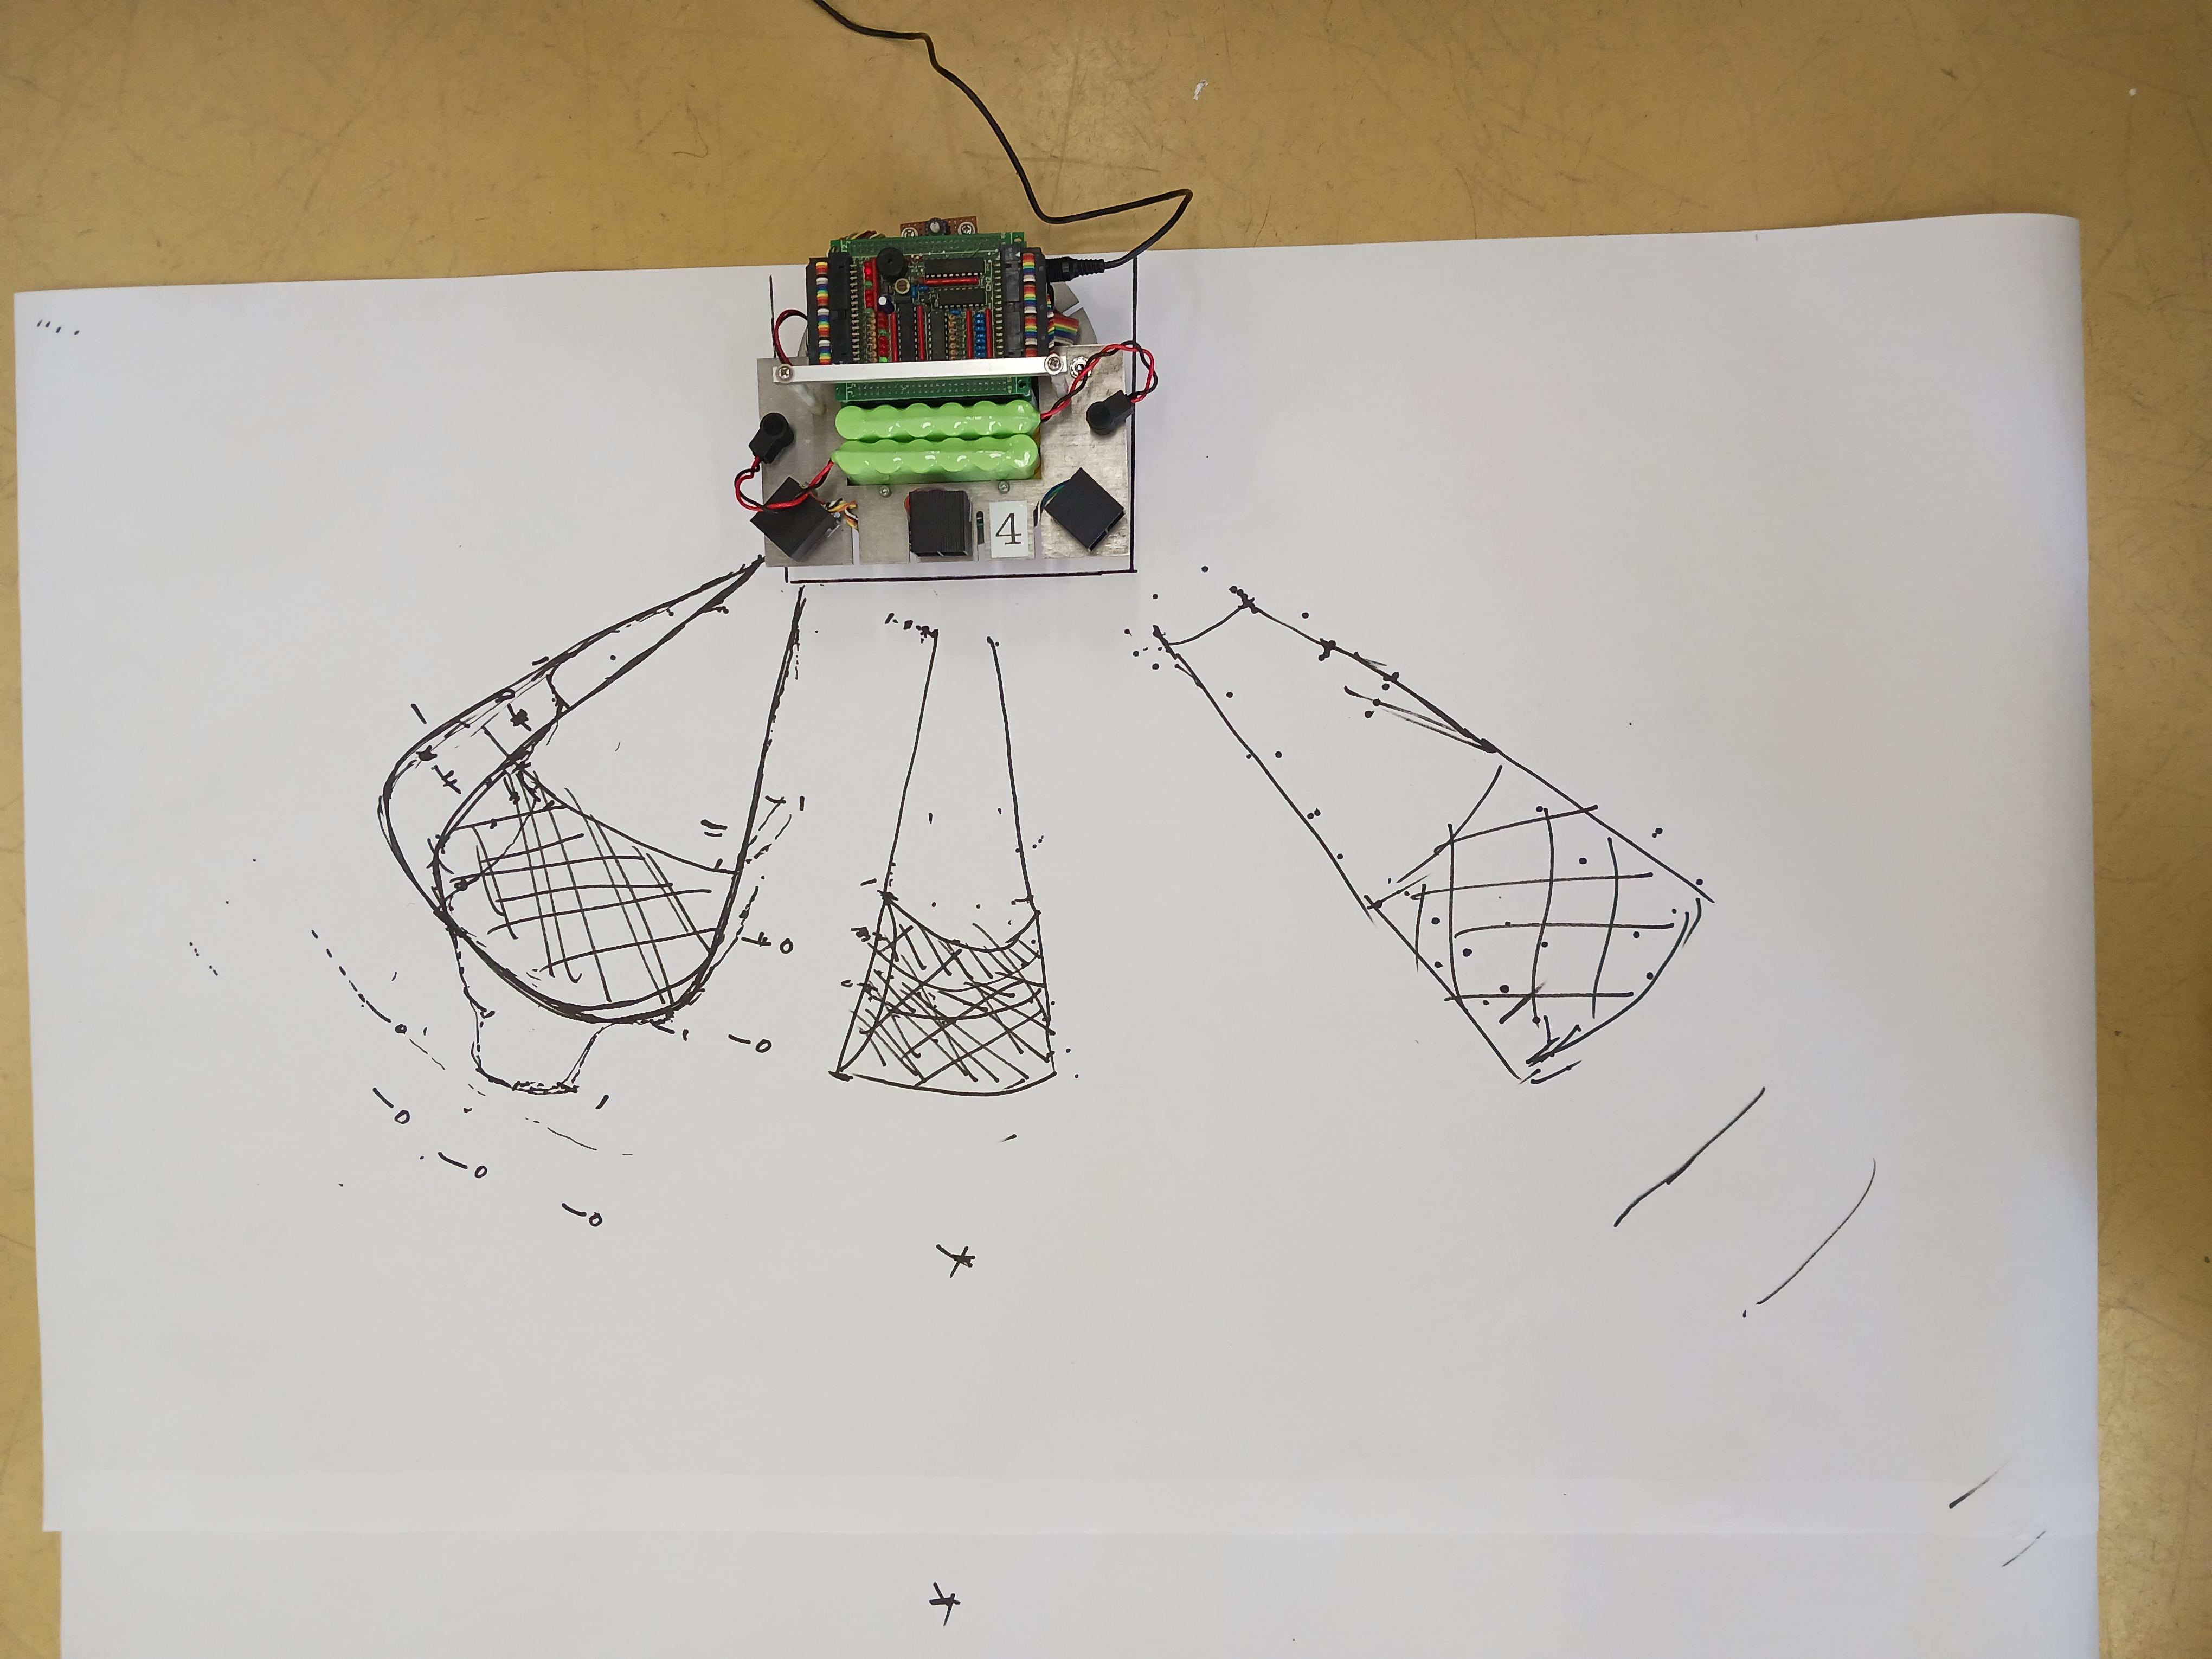
\includegraphics[width=.8\columnwidth]{img/8.jpg}
  \caption{赤外線センサの2次元的な範囲}
  \label{niji}
  \end{center}
\end{figure}

\section{演習9}
\subsection{実行プログラム}
実行プログラムをソースコード\ref{s9}に示す。
\begin{lstlisting}[caption=演習9のプログラム,label=s9]
#include <stdio.h>
#include <dos.h>
#include "v25.h"
#include "ms.h"
  
int main(){
  long cl, cr, ct;
  
  ms_enc_init();
  printf("%c[2J", 0x1b);
  while(1){
     ms_read_c(&cl, &cr, &ct);
  
    printf("%c[01;01H", 0x1b);
    printf("L:%10ld\n", cl);
    printf("R:%10ld\n", cr);
    printf("T:%10ld\n", ct);
  }
  return 0;
}
\end{lstlisting}

\subsection{実行結果}
タイヤを正回転させることで、
左右のモータのロータリーエンコーダの値が加算されて出力される。
タイヤを逆回転させると、減算されて出力される。

\section{演習10}
\subsection{実行プログラム}
実行プログラムをソースコード\ref{s10}に示す。
\begin{lstlisting}[caption=演習10のプログラム,label=s10]
#include <stdio.h>
#include <dos.h>
#include "v25.h"
#include "ms.h"
  
int main(){
  int i;
  long cl, cr, ct;
  long f[3] = {0, 0, 1};
  long f_old[3] = {0, 0, 0};
  float a_l, a_r, v_l, v_r;
  
  ms_enc_init();
  printf("%c[2J", 0x1b);
  while(1){
    ms_read_c(&cl, &cr, &ct);
  
    f[0] = cl;
    f[1] = cr;
    f[2] = ct*3/1000;
  
  
    a_l = (1000/3)*(f[0] - f_old[0])/(400*19.225);
    a_r = (1000/3)*(f[1] - f_old[1])/(400*19.225);
    v_l = (60*a_l);
    v_r = (60*a_r);
  
    printf("%c[01;01H", 0x1b);
    printf("a_l:%10lf\n", a_l);
    printf("a_r:%10lf\n", a_r);
    printf("v_l:%10lf\n", v_l);
    printf("v_r:%10lf\n", v_r);
          
    printf("T:%10ld\n", ct*3/1000);
  
    for (i = 0; i < 2; i++){
      f_old[i] = f[i];
    }
 
  }
  return 0;
}
\end{lstlisting}

\subsection{実行結果}
左右のロータリーエンコーダの値をモータの回転数に変換され、
モータの回転数の瞬時値が出力される。

\section{演習11}
\subsection{実行プログラム}
実行プログラムをソースコード\ref{s11}に示す。

\begin{lstlisting}[caption=演習11のプログラム,label=s11]
#include <stdio.h>
#include <dos.h>
#include "v25.h"
#include "ms.h"

int main(){
  int i;
  int vl, vr;
  long ct;
  
  ms_motor_init();
  ms_motor_on();
  
  printf("%c[2J", 0x1b);
  
  for(i=0; i>=-127; i--){
    ms_set_pwm(i, i);
    ms_wait(50);
  }
  
  for(i=-127; i<=127; i++){
    ms_set_pwm(i, i);
    ms_wait(50);
    ms_read_v(&vl, &vr, &ct);
    printf("%c[01;01H", 0x1b);
    printf("pwm:%5d\n", i);
    printf("vl:%7d\n", vl);
    printf("vr:%7d\n", vr);
  }
  
  for(i=127; i>=0; i--){
    ms_set_pwm(i, i);
    ms_wait(50);
  }
  
  ms_motor_off();
  return 0;
}
\end{lstlisting}

\subsection{実行結果}
左右のモータが回転し、その時の回転速度がJTW上に表示される。

\section{演習12}
\subsection{実行プログラム}
実行プログラムをソースコード\ref{s12}に示す。
\begin{lstlisting}[caption=演習12のプログラム,label=s12]
#include <stdio.h>
#include <dos.h>
#include "v25.h"
#include "ms.h"
#include<process.h>
  
int main(){
  int i;
  int vl, vr;
  long ct;
  FILE *fp;
  
  ms_motor_init();
  ms_motor_on();
  
  printf("%c[2J", 0x1b);
  
  for(i=0; i>=-127; i--){
    ms_set_pwm(i, i);
    ms_wait(50);
  }
  
  /*ファイルのオープン*/
  if ((fp = fopen("12.csv","wt"))==NULL)
  {
    printf("Can't open file.\n");
    exit(1);
  }
  
  for(i=-127; i<=127; i++){
    ms_set_pwm(i, i);
    ms_wait(50);
    ms_read_v(&vl, &vr, &ct);
    printf("%c[01;01H", 0x1b);
    printf("pwm:%5d\n", i);
    printf("vl:%7d\n", vl);
    printf("vr:%7d\n", vr);
  
    fprintf(fp,"%5d,%7d,%7d\n",i,vl,vr); /*pwm値と左右回転速度の書き込み*/
  }
  
  for(i=127; i>=0; i--){
    ms_set_pwm(i, i);
    ms_wait(50);
  }
  
  ms_motor_off();
  /*ファイルのクローズ*/
  fclose(fp);
  return 0;
}
\end{lstlisting}

\subsection{実行結果}
左右のモータのPWM値と回転速度のデータファイル "12.csv" が作成される。
12.csvに置けるモータの回転数の特性を図\ref{pwm}に示す。

\begin{figure}[H]
  \begin{center}
  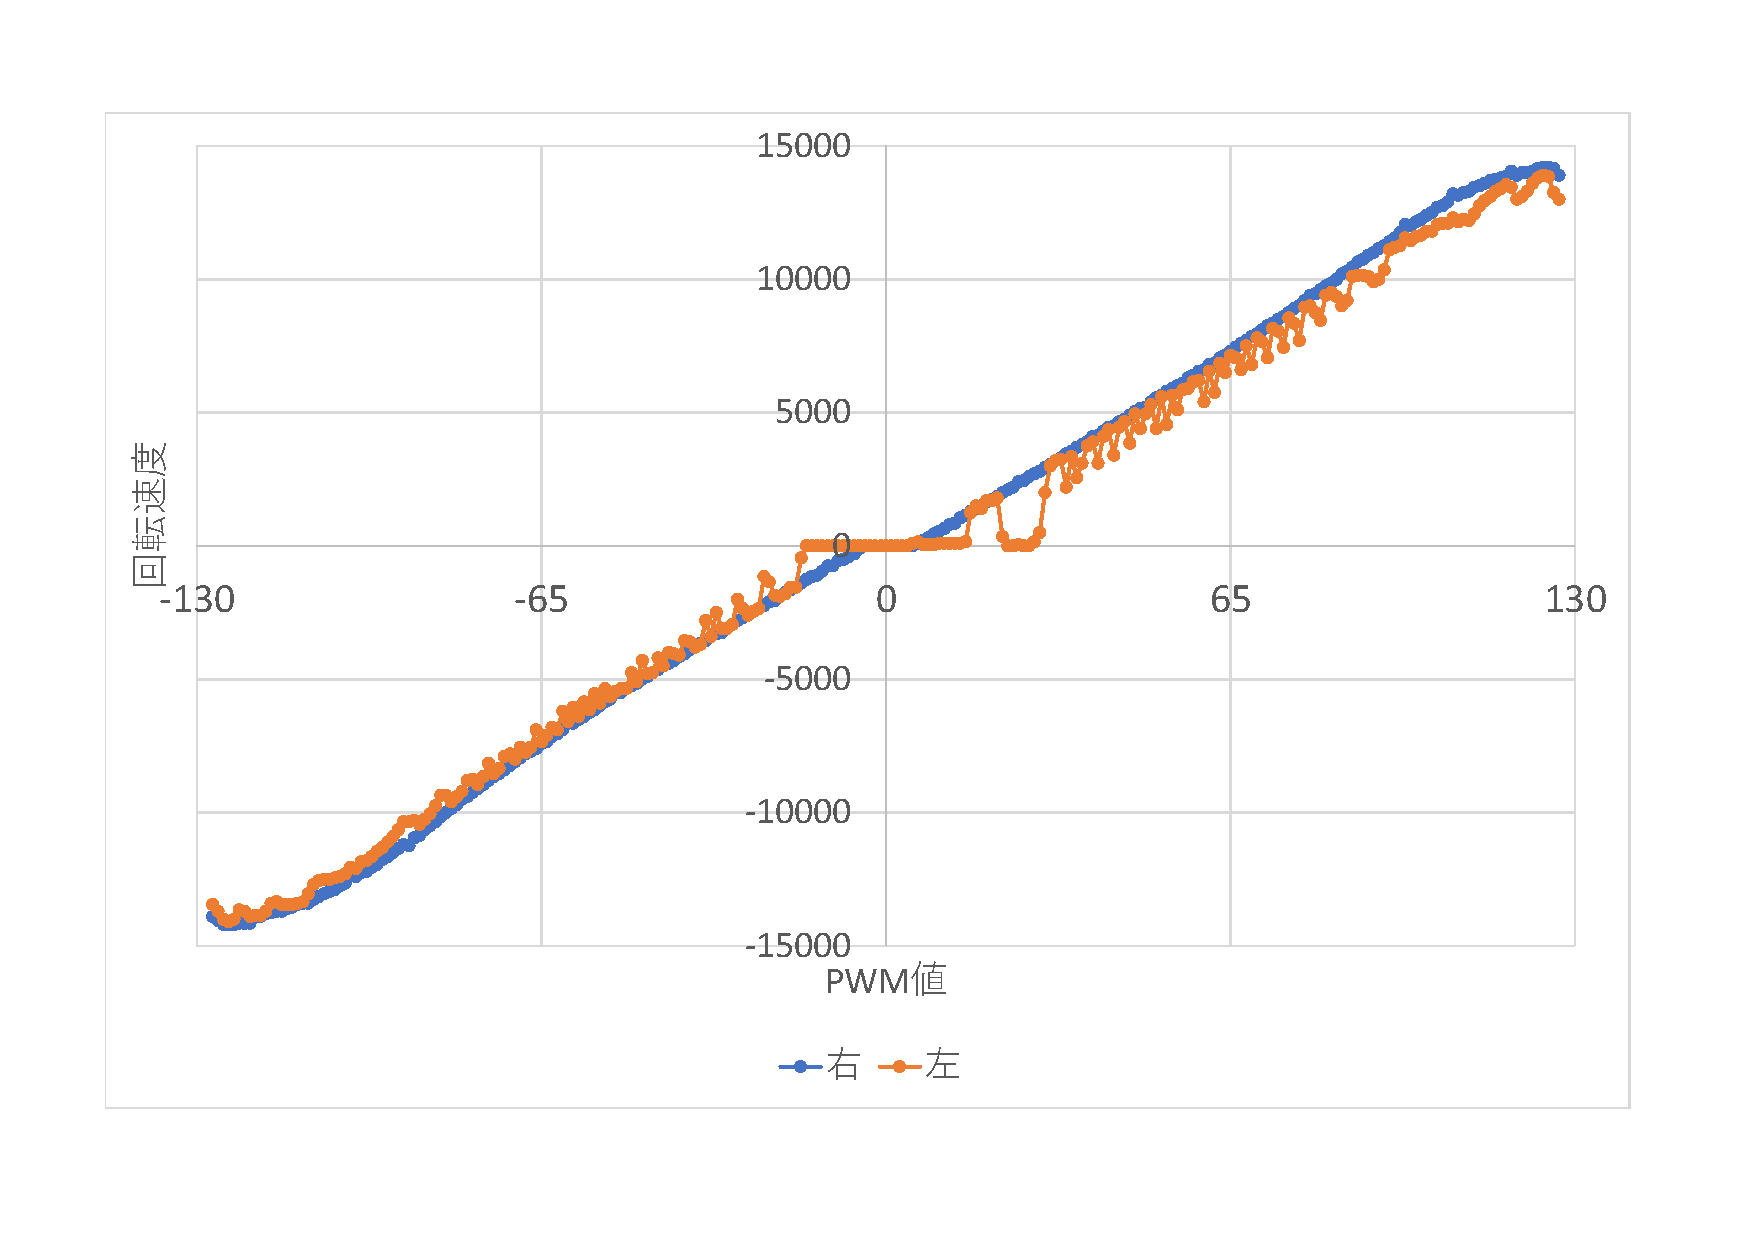
\includegraphics[width=\columnwidth]{img/12.pdf}
  \caption{左右のモータの回転数の特性}
  \label{pwm}
  \end{center}
\end{figure}

\section{演習13}
\subsection{実行プログラム}
実行プログラムをソースコード\ref{s13}に示す。
\begin{lstlisting}[caption=演習13のプログラム,label=s13]
#include <stdio.h>
#include <process.h> /*exit関数の定義*/
#include <dos.h>
#include "v25.h"
#include "ms.h"
  
#define DMAX 500 /*保存するデータ数*/
  
int main(){
  int i;
  int kp, ki_inv;
  int vrefl, vrefr;
  int vl[DMAX], vr[DMAX];
  long ct, ctm, t[DMAX];
  FILE *fp;
  
  ms_init();
  
  kp = ms_read_dip();
  ki_inv = 10000;
  vrefl = 5000;
  vrefr = 5000;
  
  ms_motor_on();
  ms_read_v(&vl[0], &vr[0], &ctm);
  ms_step_res(vrefl, vrefr, kp, ki_inv);
  for(i=1; i<DMAX; i++){
    ms_read_v(&vl[i], &vr[i], &ct);
    t[i] = ct - ctm;
      ms_wait(2);
  }
  ms_motor_off();
  
  if((fp = fopen("data.dat", "wt")) == NULL){
    printf("Can't Open File!!\n");
    exit(1);
  }
  
  for(i=1; i<DMAX; i++){
    fprintf(fp, "%7d %7d %10ld\n", vl[i], vr[i], t[i]);
  }
  fclose(fp);
  return 0;
}
\end{lstlisting}

\subsection{実行結果}
モータのステップ応答(回転速度と時間)
をデータファイルに保存する。
比例フィードバック係数$k_p$をスイッチ値(0\verb|~|15)を変化させた時の
応答グラフを図\ref{im0}\verb|~|\ref{im15}に示す。
なお、$k_p$の値は\tsuyo{7}で安定とした。
$k_p = 0 ~ 2$の場合、ロボットは前進しない。
\begin{figure}[H]
  \begin{center}
  \subfigure[$k_p=0$]{
  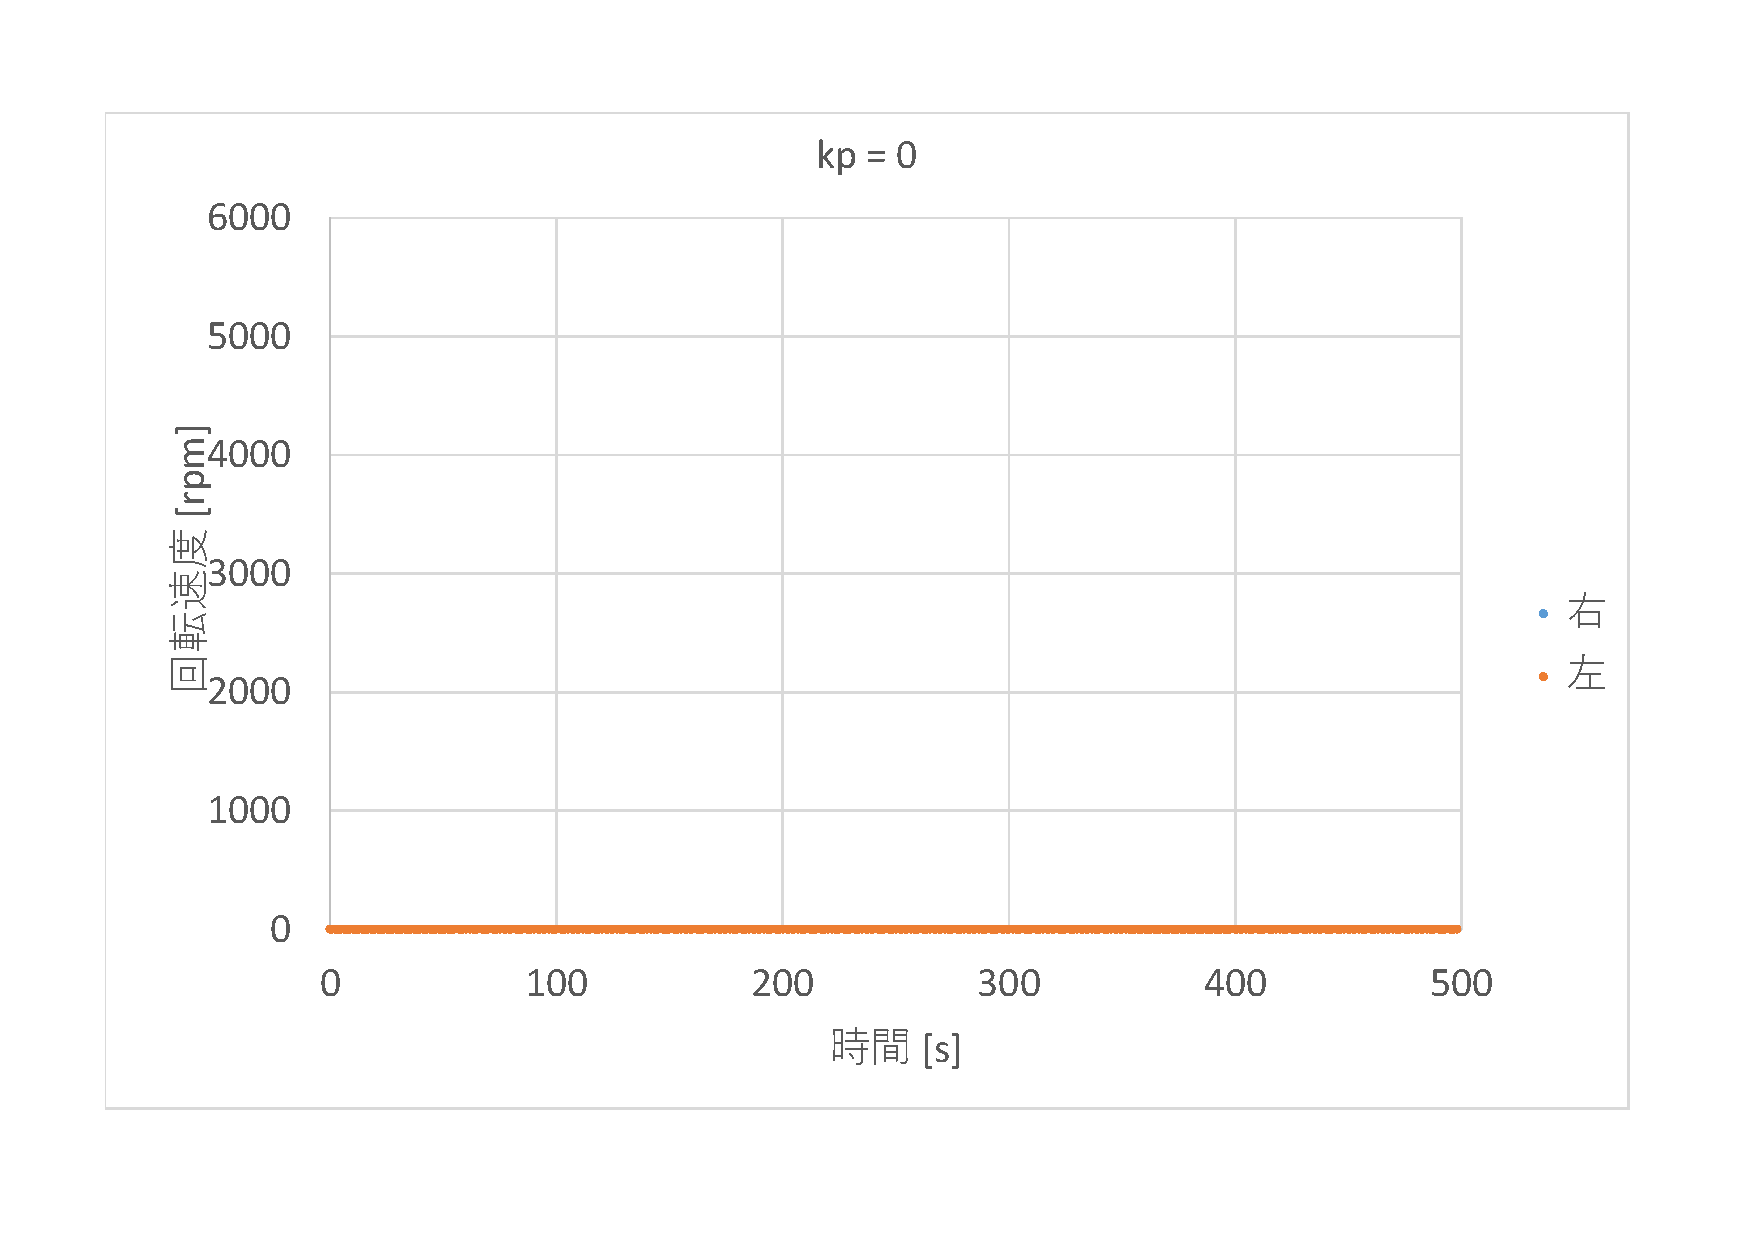
\includegraphics[width=\columnwidth]{img/13/DATA0.pdf}
  \label{im0}
  }
  \subfigure[$k_p=1$]{
  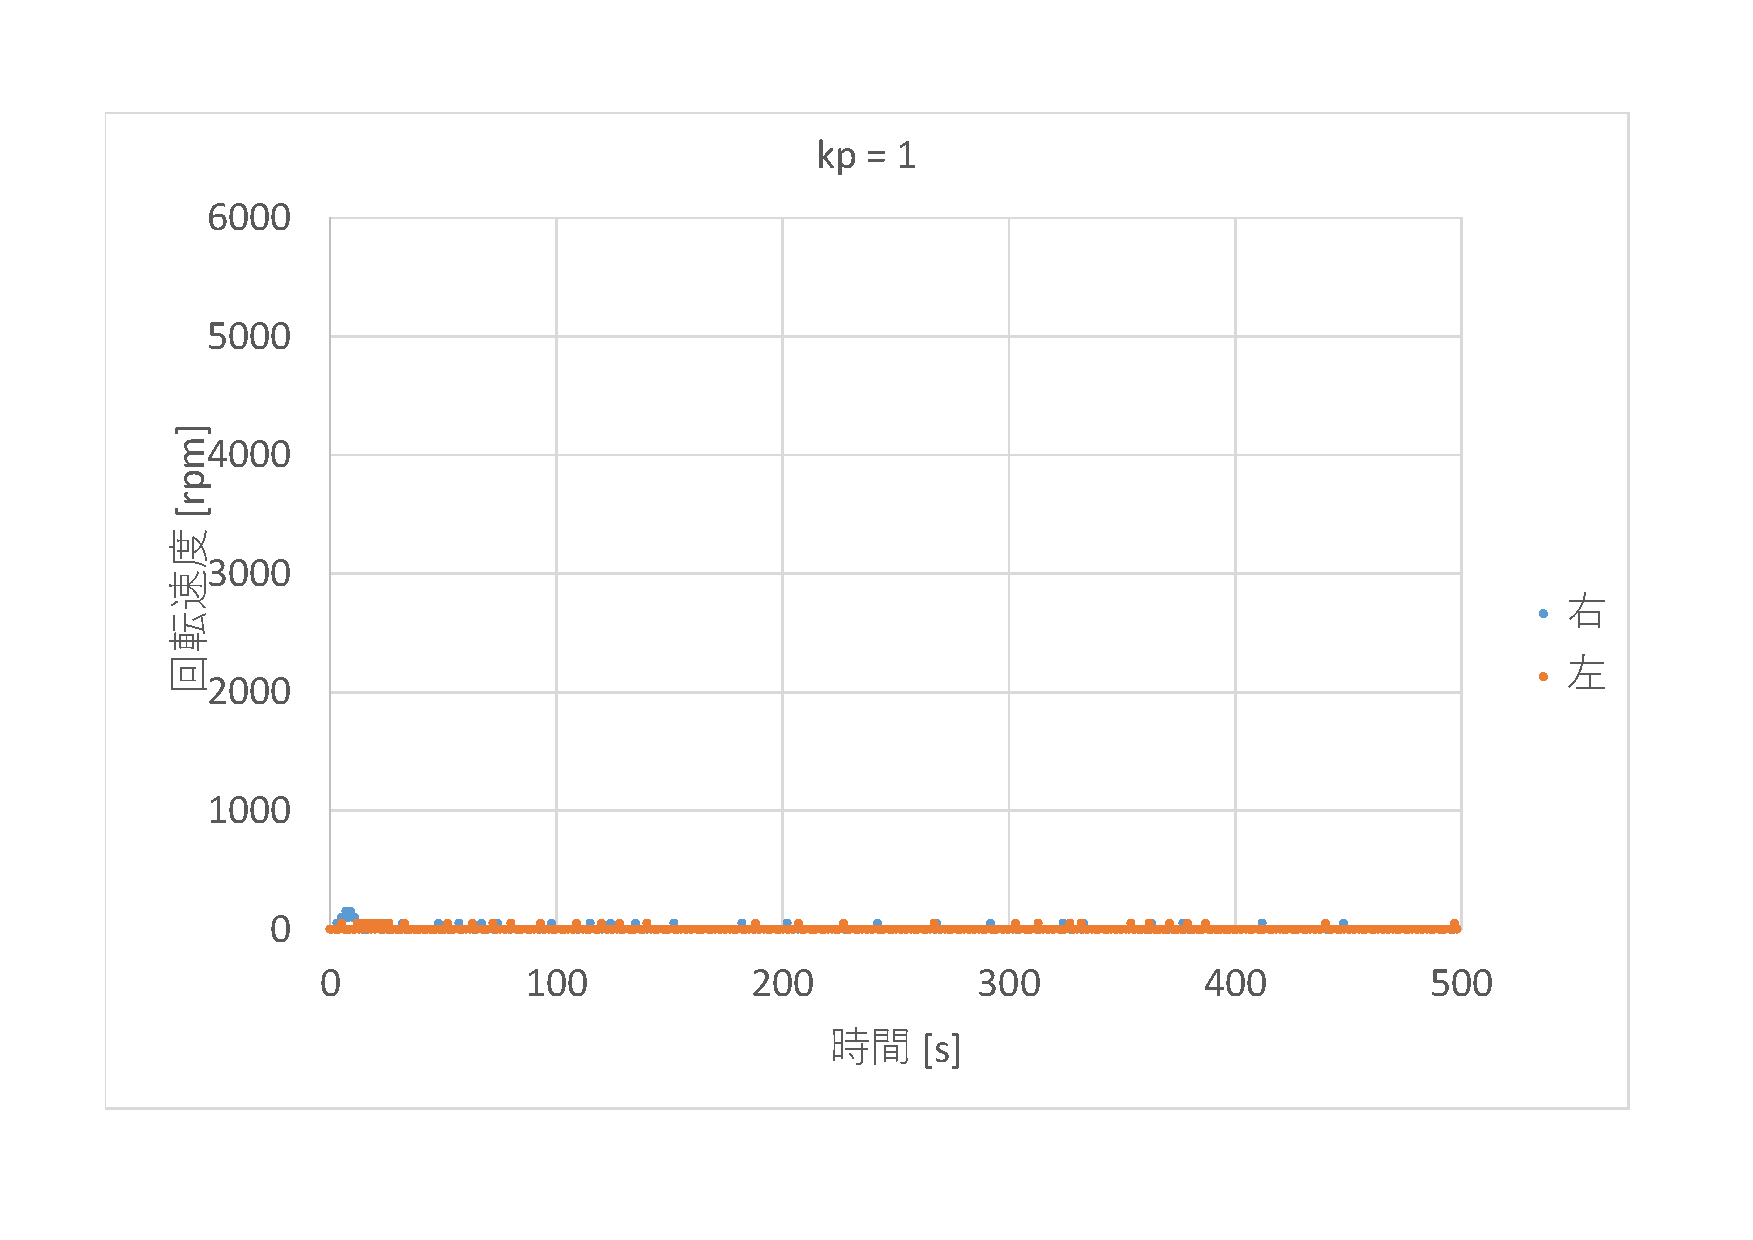
\includegraphics[width=\columnwidth]{img/13/DATA1.pdf}
  \label{im1}
  }
  \caption{ステップ応答のグラフ}
  \end{center}
\end{figure}

\begin{figure}[H]
  \begin{center}
  \subfigure[$k_p=2$]{
  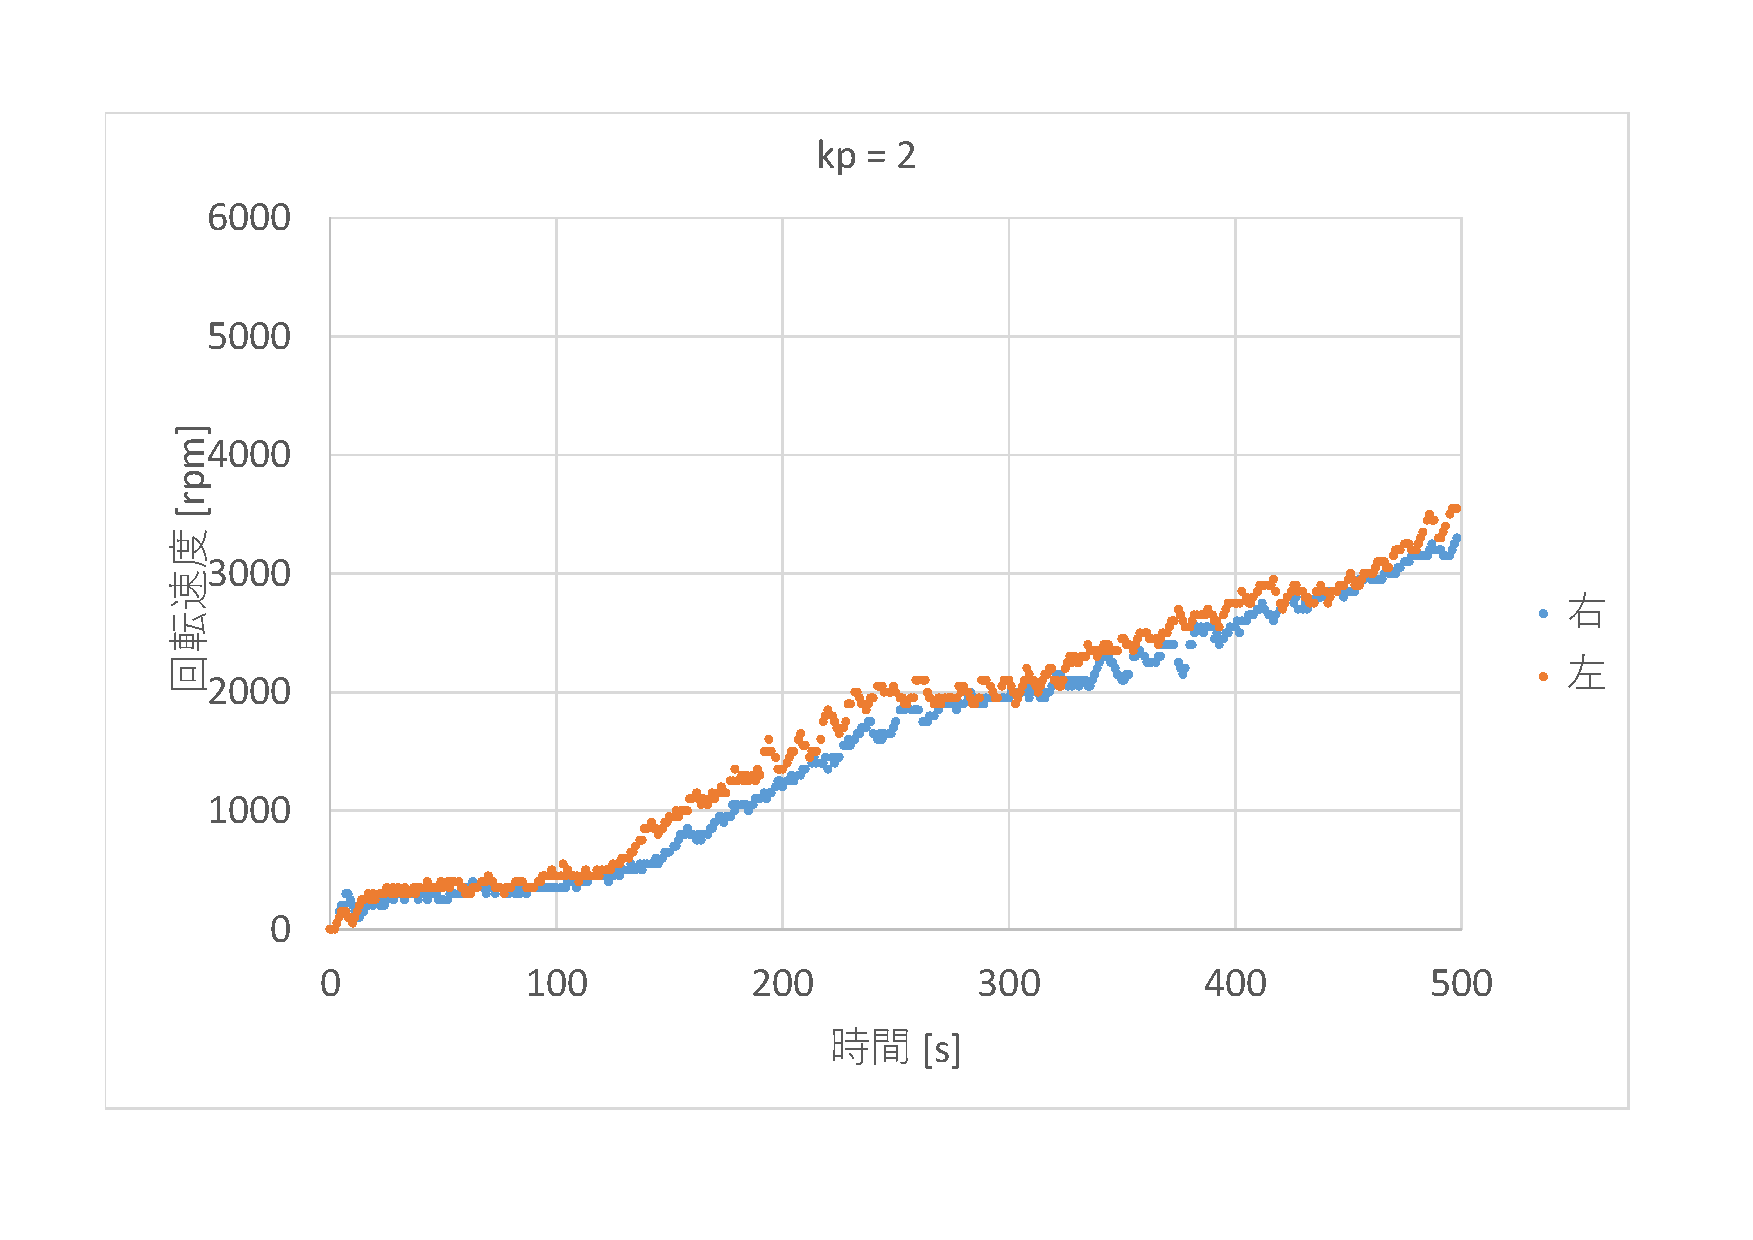
\includegraphics[width=\columnwidth]{img/13/DATA2.pdf}
  \label{im2}
  }
  \subfigure[$k_p=3$]{
  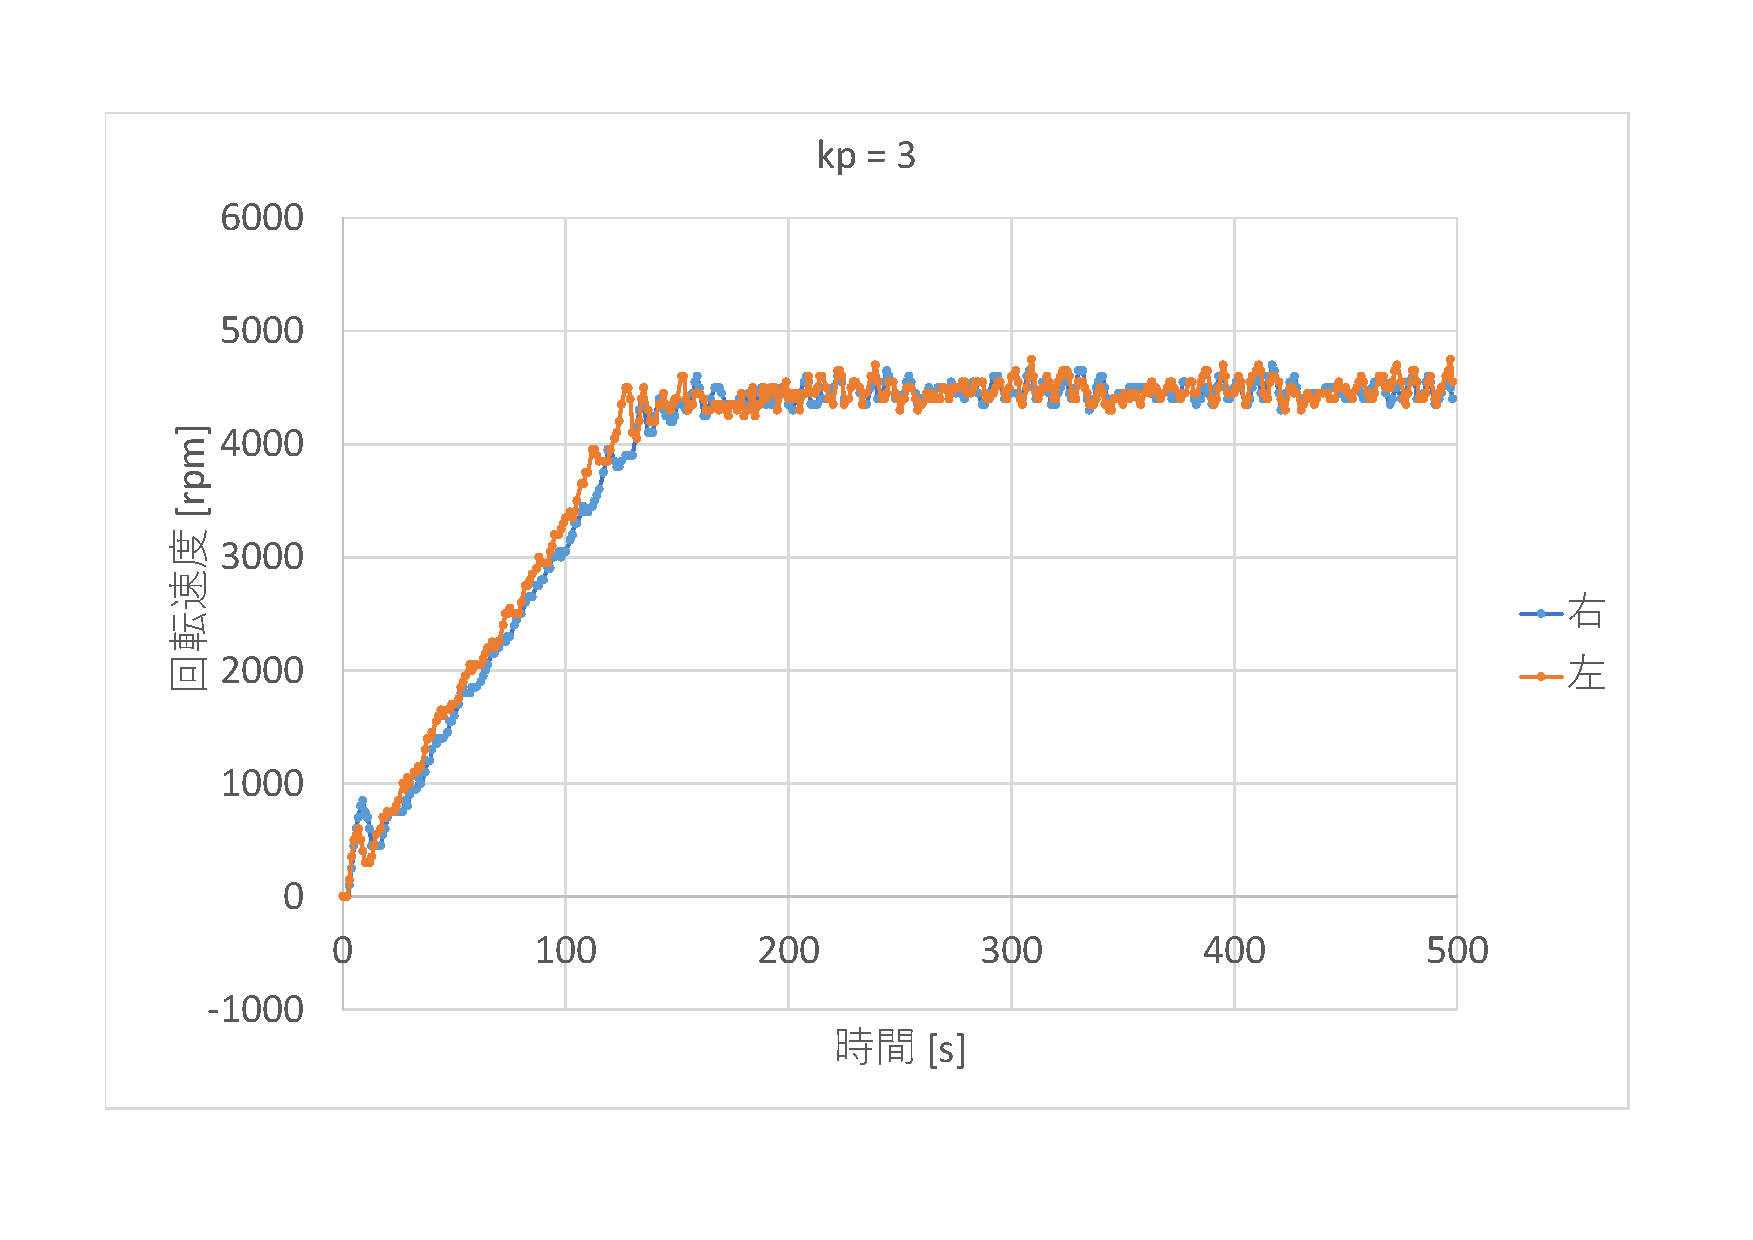
\includegraphics[width=\columnwidth]{img/13/DATA3.pdf}
  \label{im3}
  }
  \caption{ステップ応答のグラフ}
  \end{center}
\end{figure}

\begin{figure}[H]
  \begin{center}
  \subfigure[$k_p=4$]{
  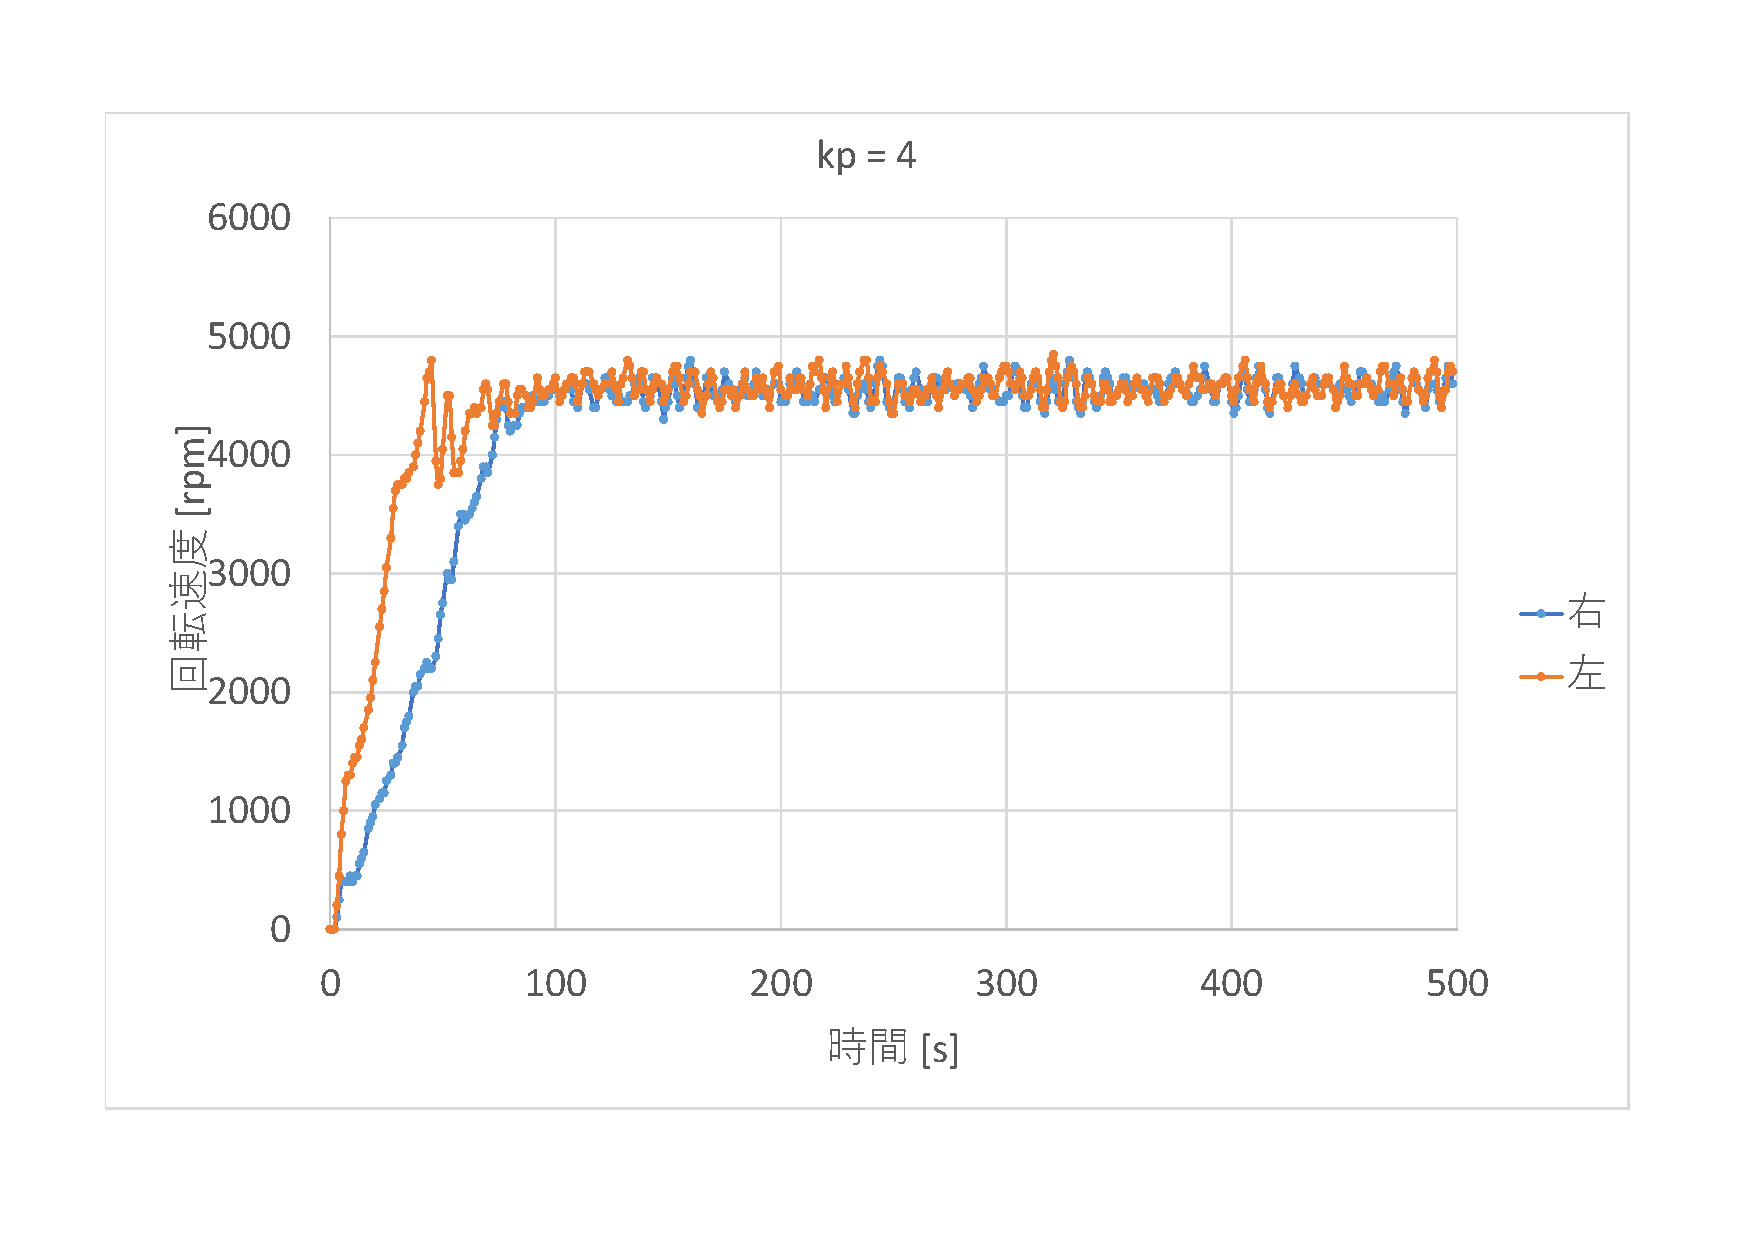
\includegraphics[width=\columnwidth]{img/13/DATA4.pdf}
  \label{im4}
  }
  \subfigure[$k_p=5$]{
  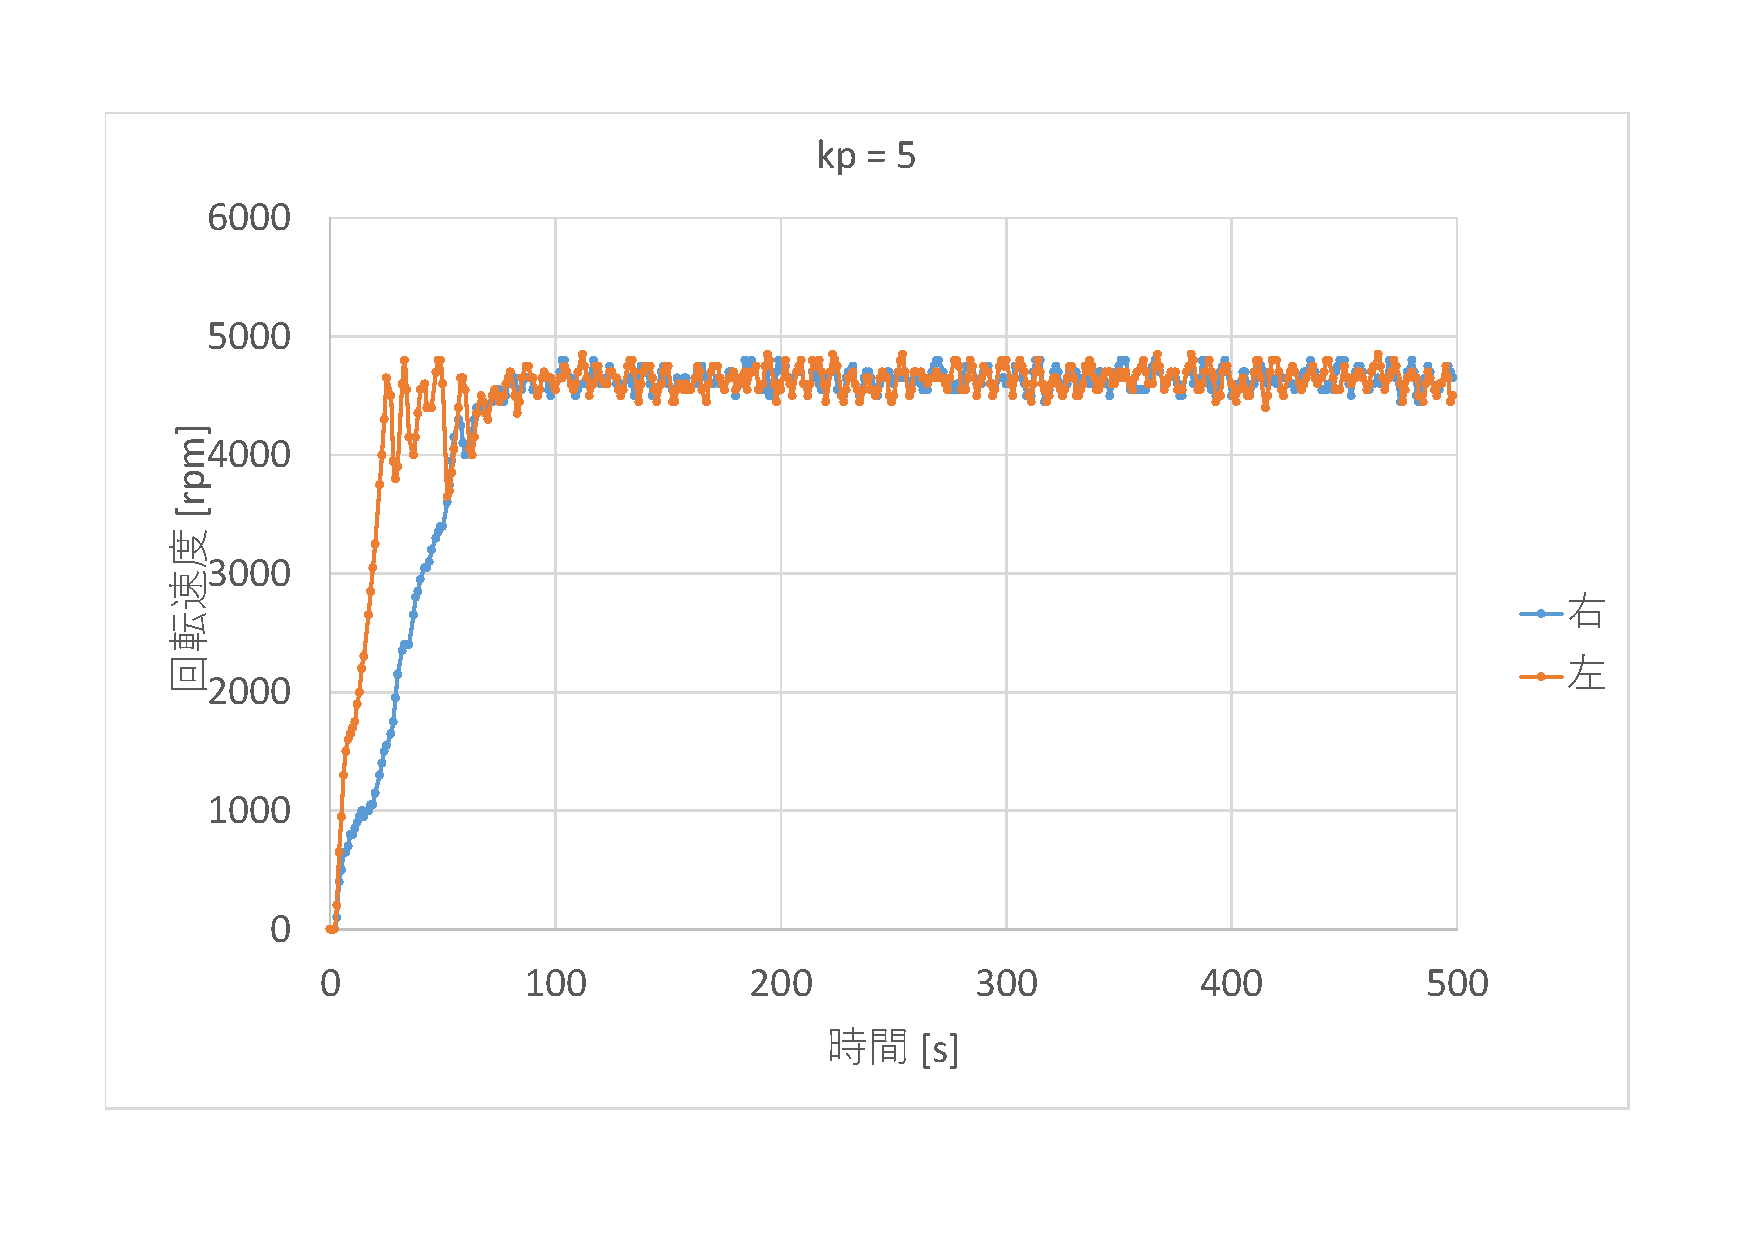
\includegraphics[width=\columnwidth]{img/13/DATA5.pdf}
  \label{im5}
  }
  \caption{ステップ応答のグラフ}
  \end{center}
\end{figure}

\begin{figure}[H]
  \begin{center}  
  \subfigure[$k_p=6$]{
  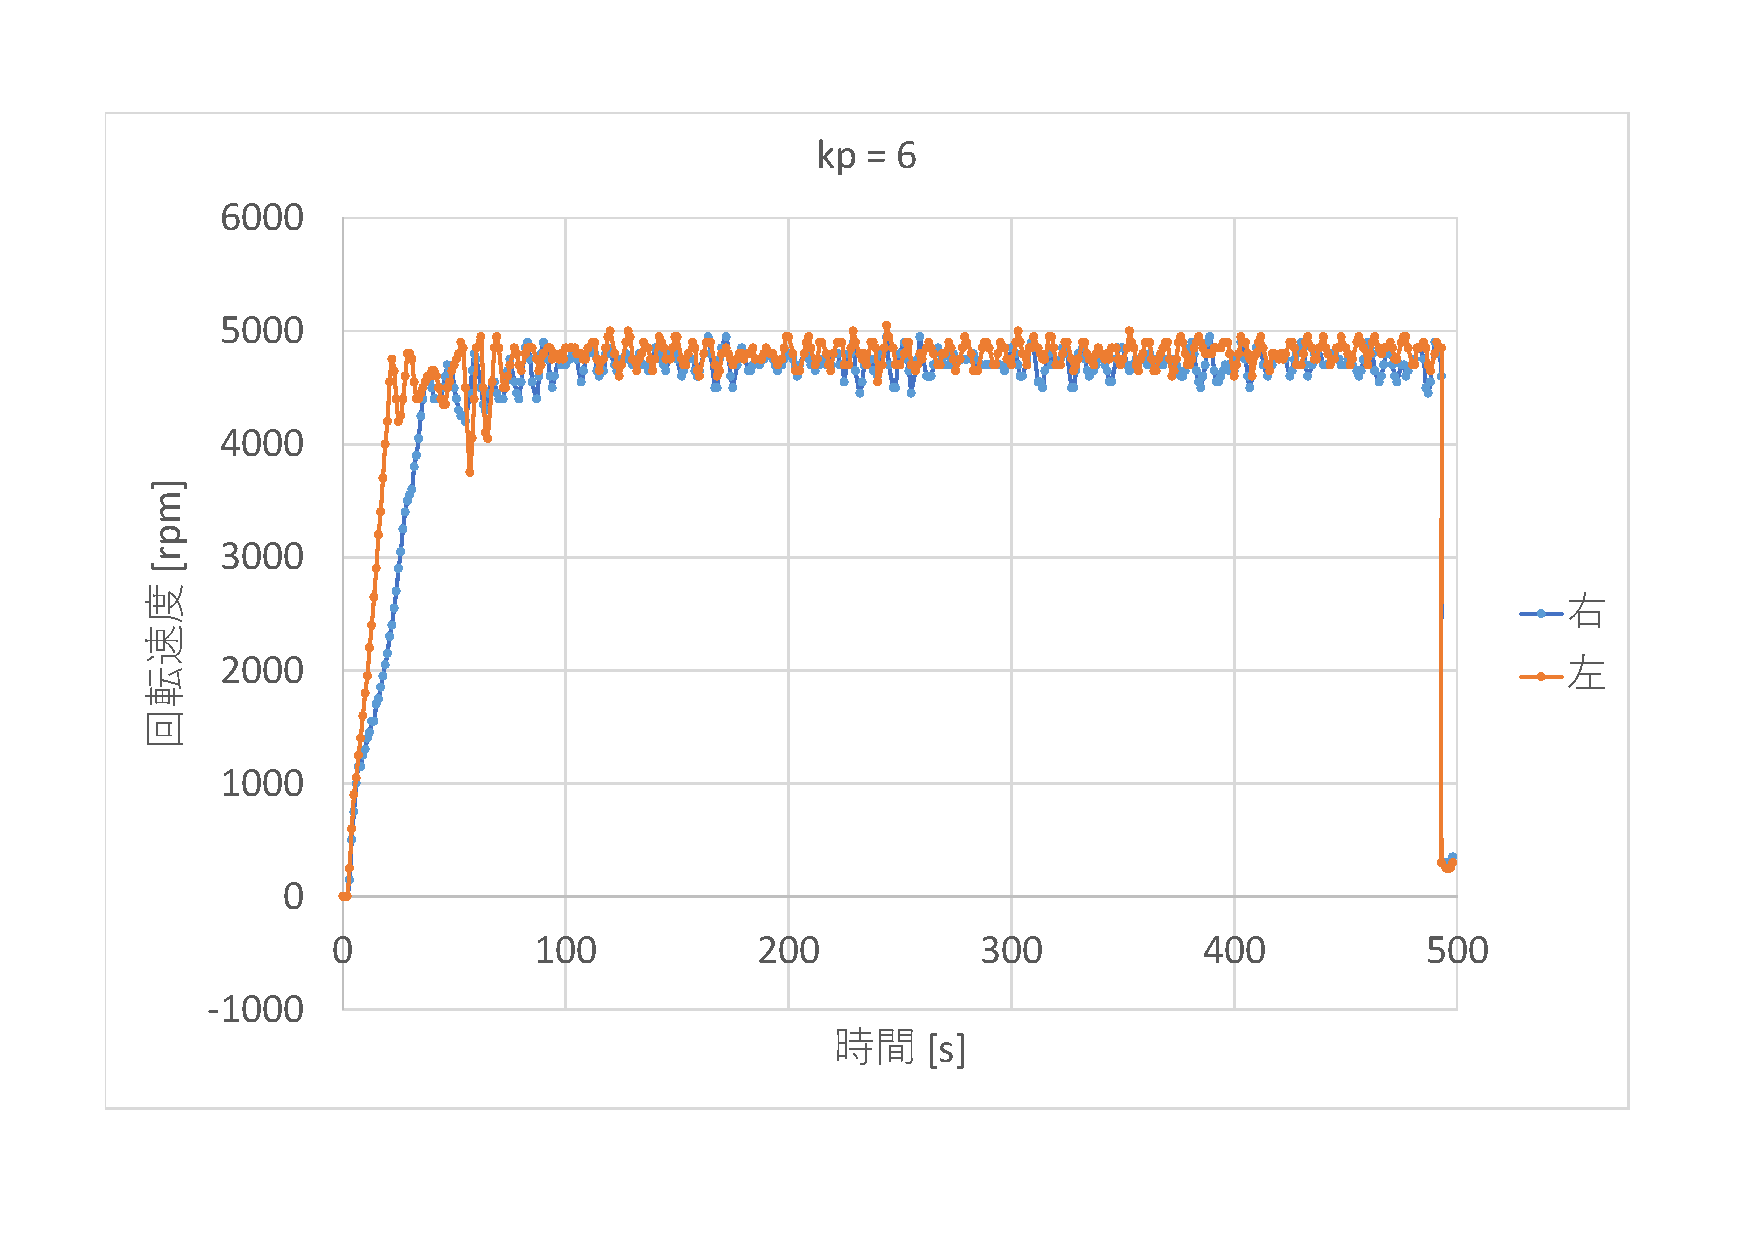
\includegraphics[width=\columnwidth]{img/13/DATA6.pdf}
  \label{im6}
  }
  \subfigure[$k_p=7$]{
  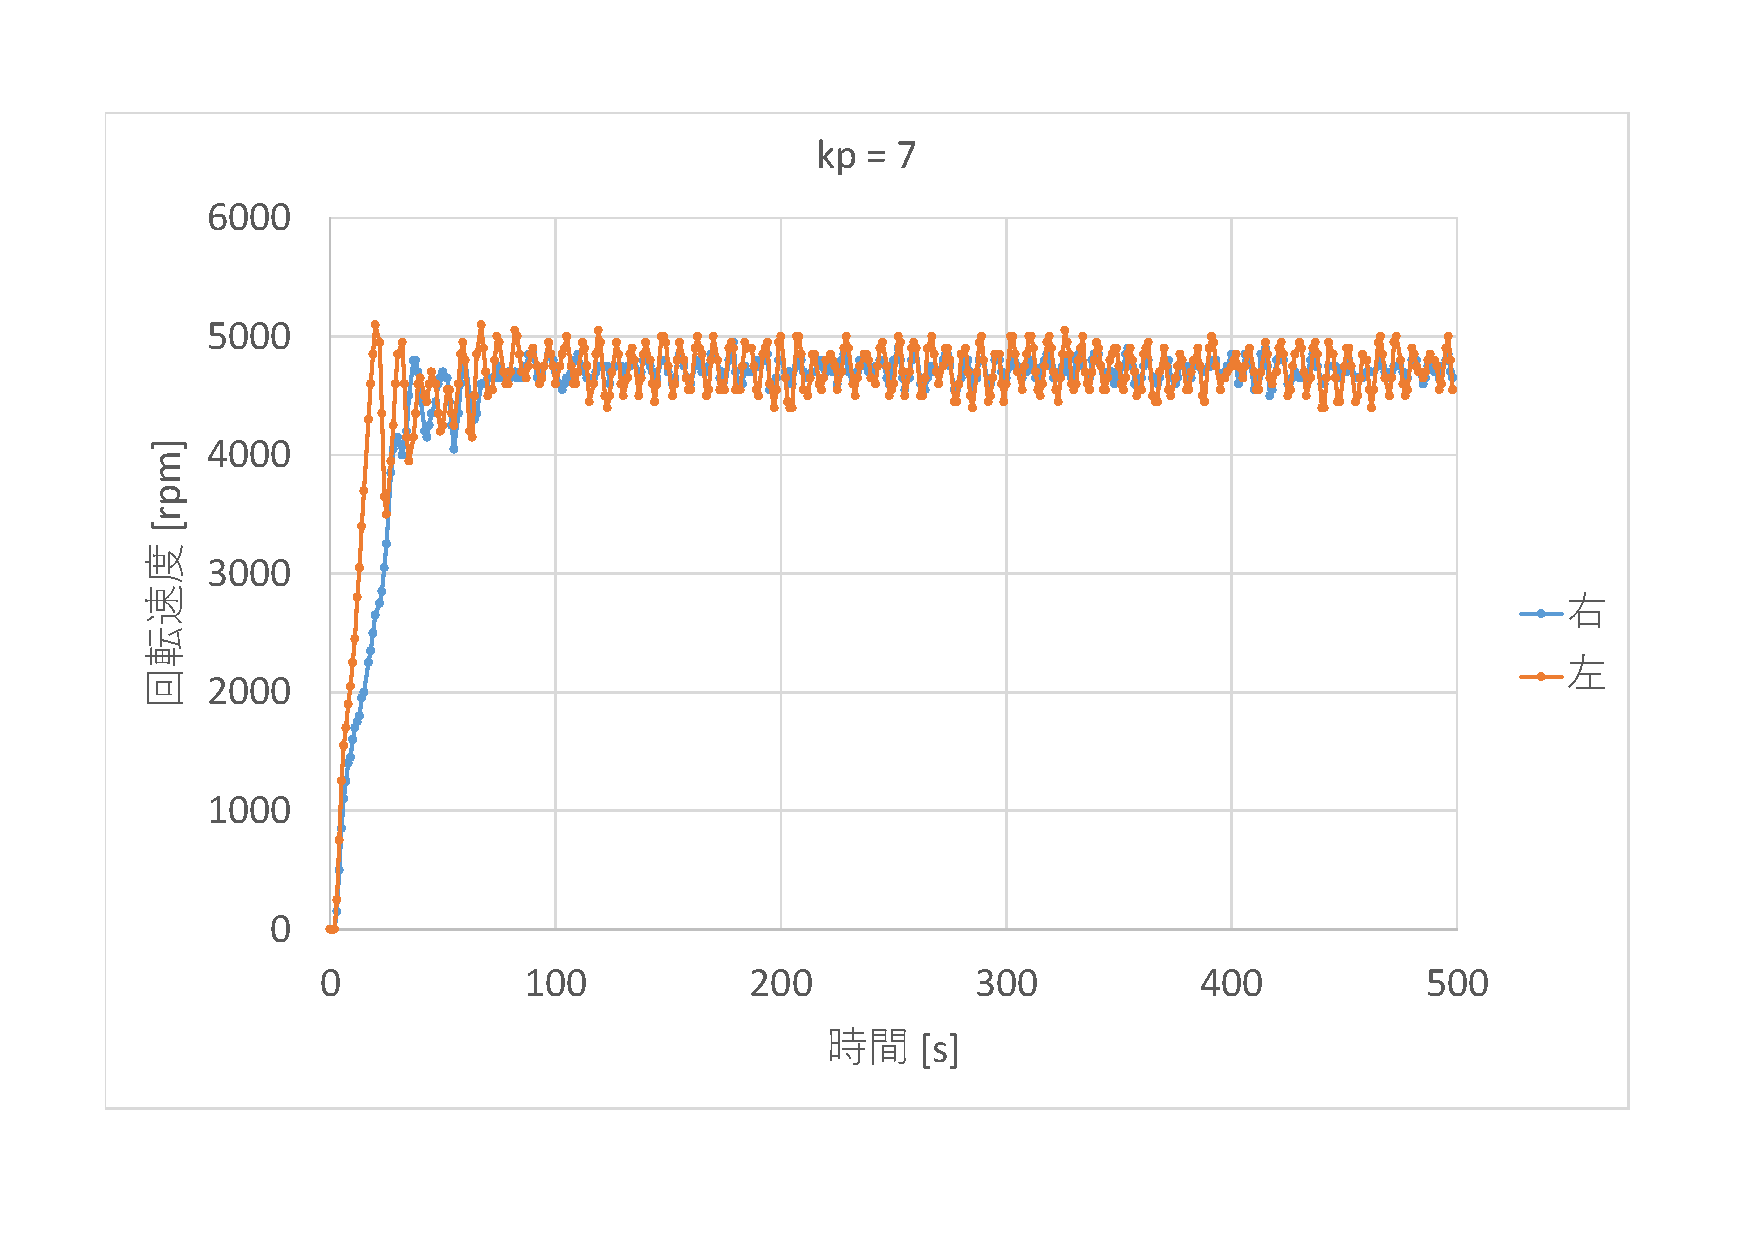
\includegraphics[width=\columnwidth]{img/13/DATA7.pdf}
  \label{im7}
  }
  \caption{ステップ応答のグラフ}
  \end{center}
\end{figure}

\begin{figure}[H]
  \begin{center}
  \subfigure[$k_p=8$]{
  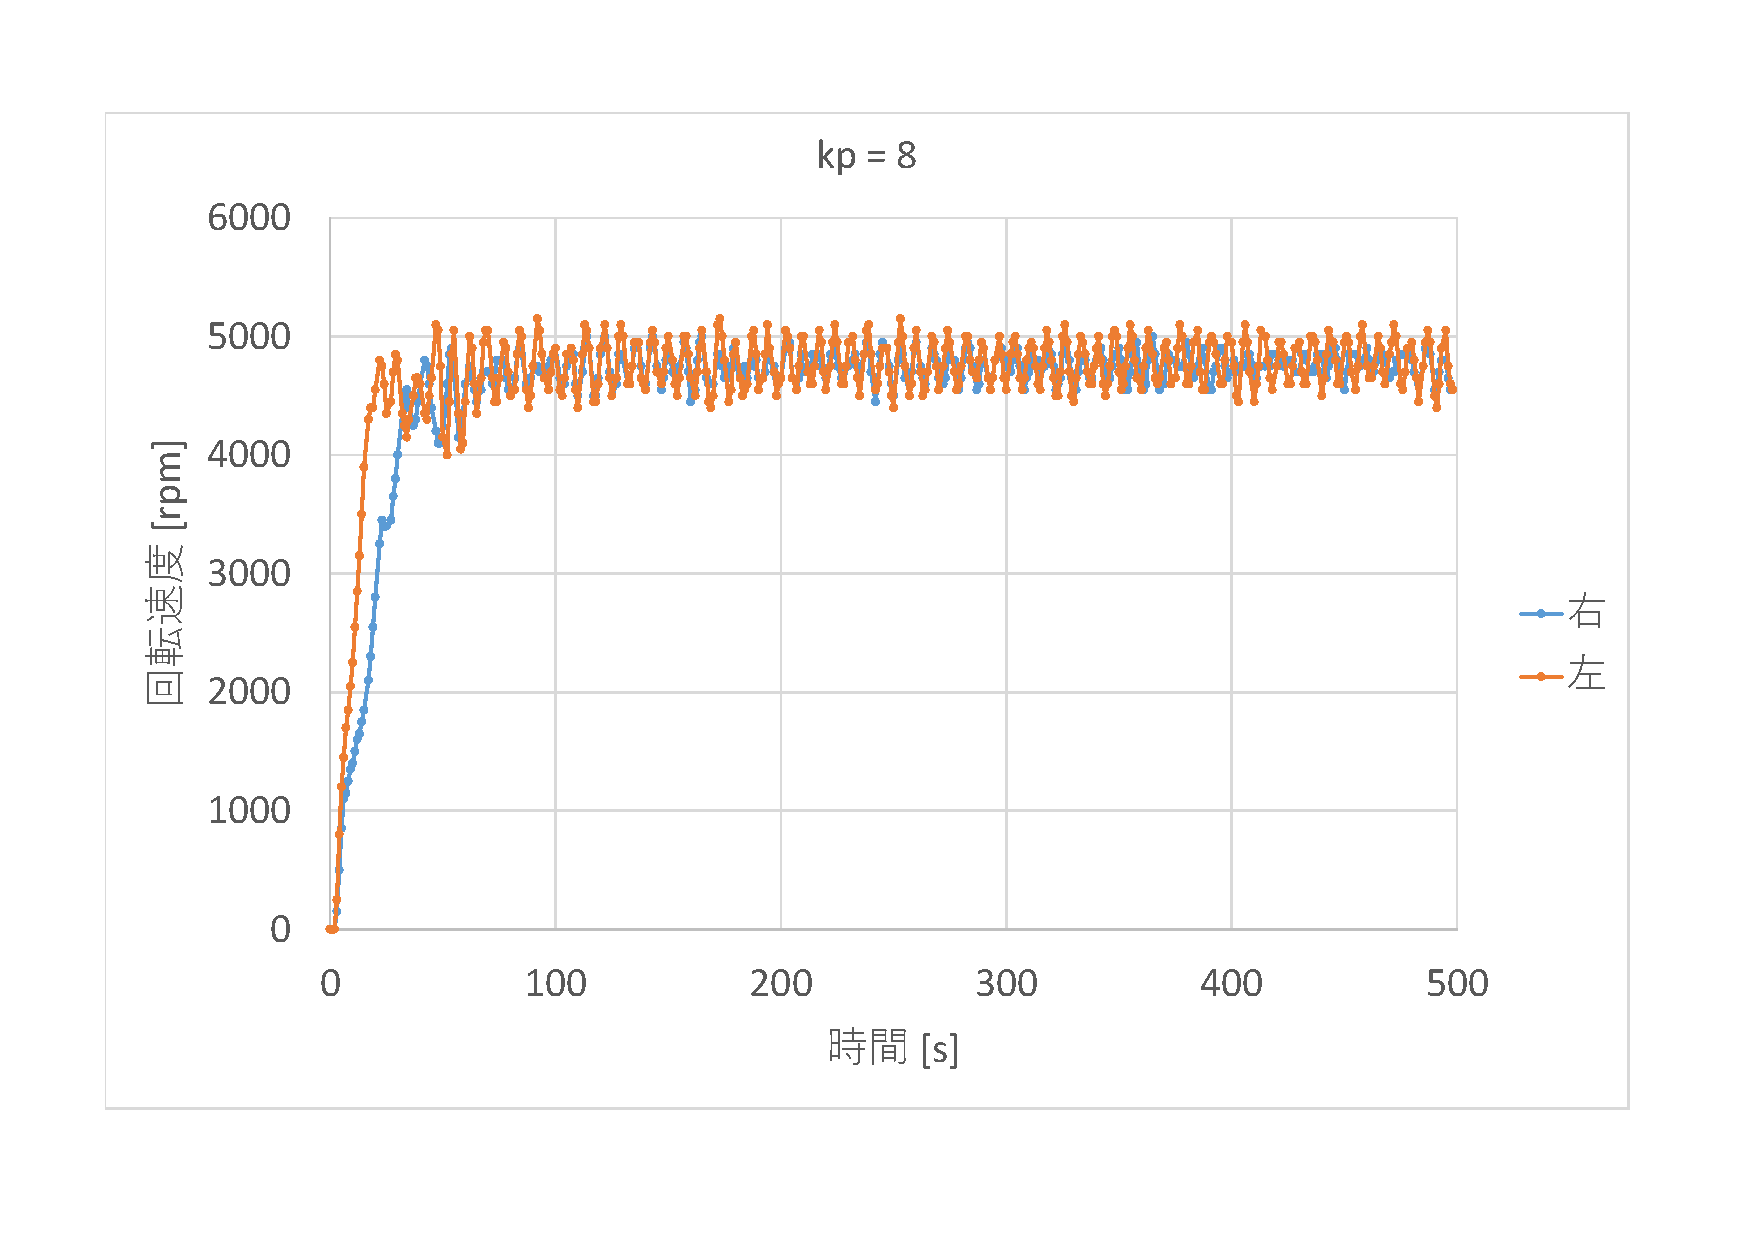
\includegraphics[width=\columnwidth]{img/13/DATA8.pdf}
  \label{im8}
  }
  \subfigure[$k_p=9$]{
  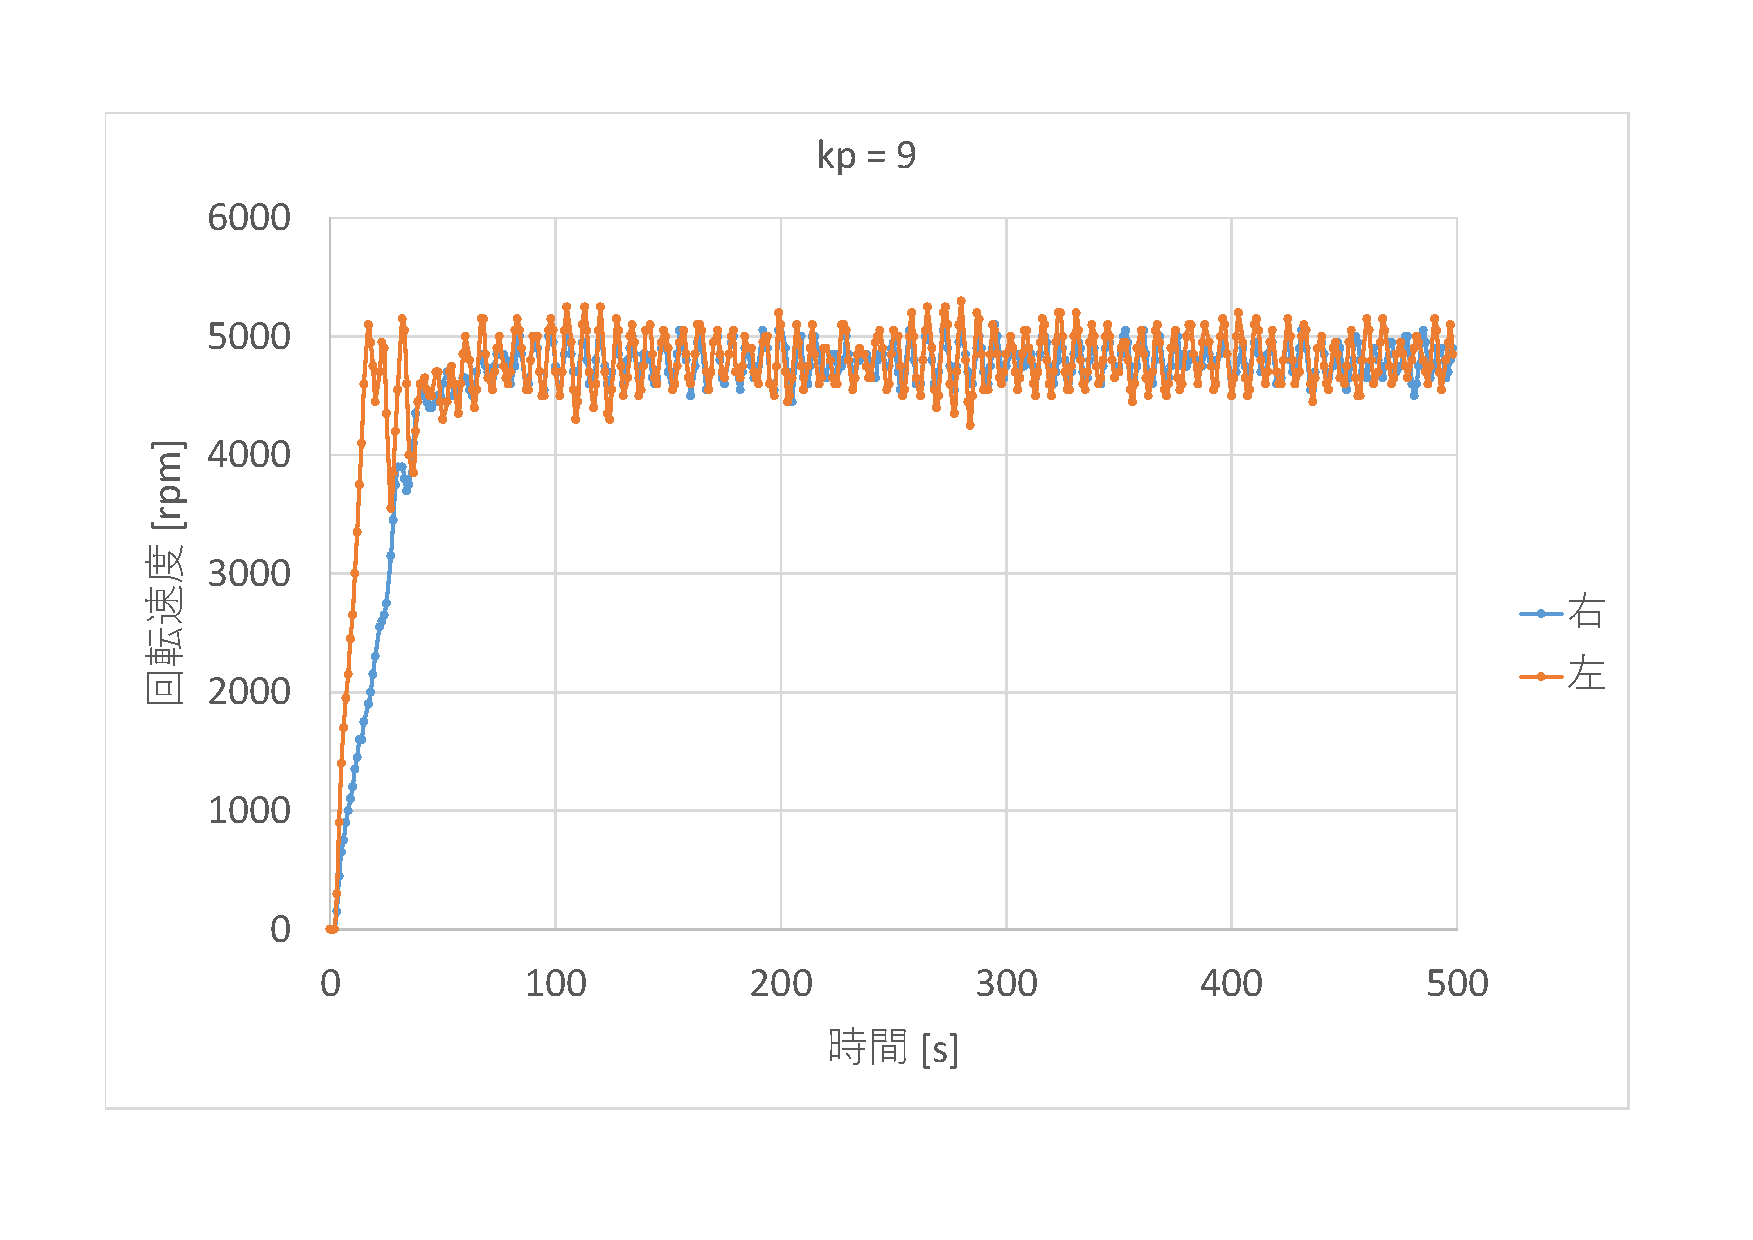
\includegraphics[width=\columnwidth]{img/13/DATA9.pdf}
  \label{im9}
  }
  \caption{ステップ応答のグラフ}
  \end{center}
\end{figure}

\begin{figure}[H]
  \begin{center}
  \subfigure[$k_p=10$]{
  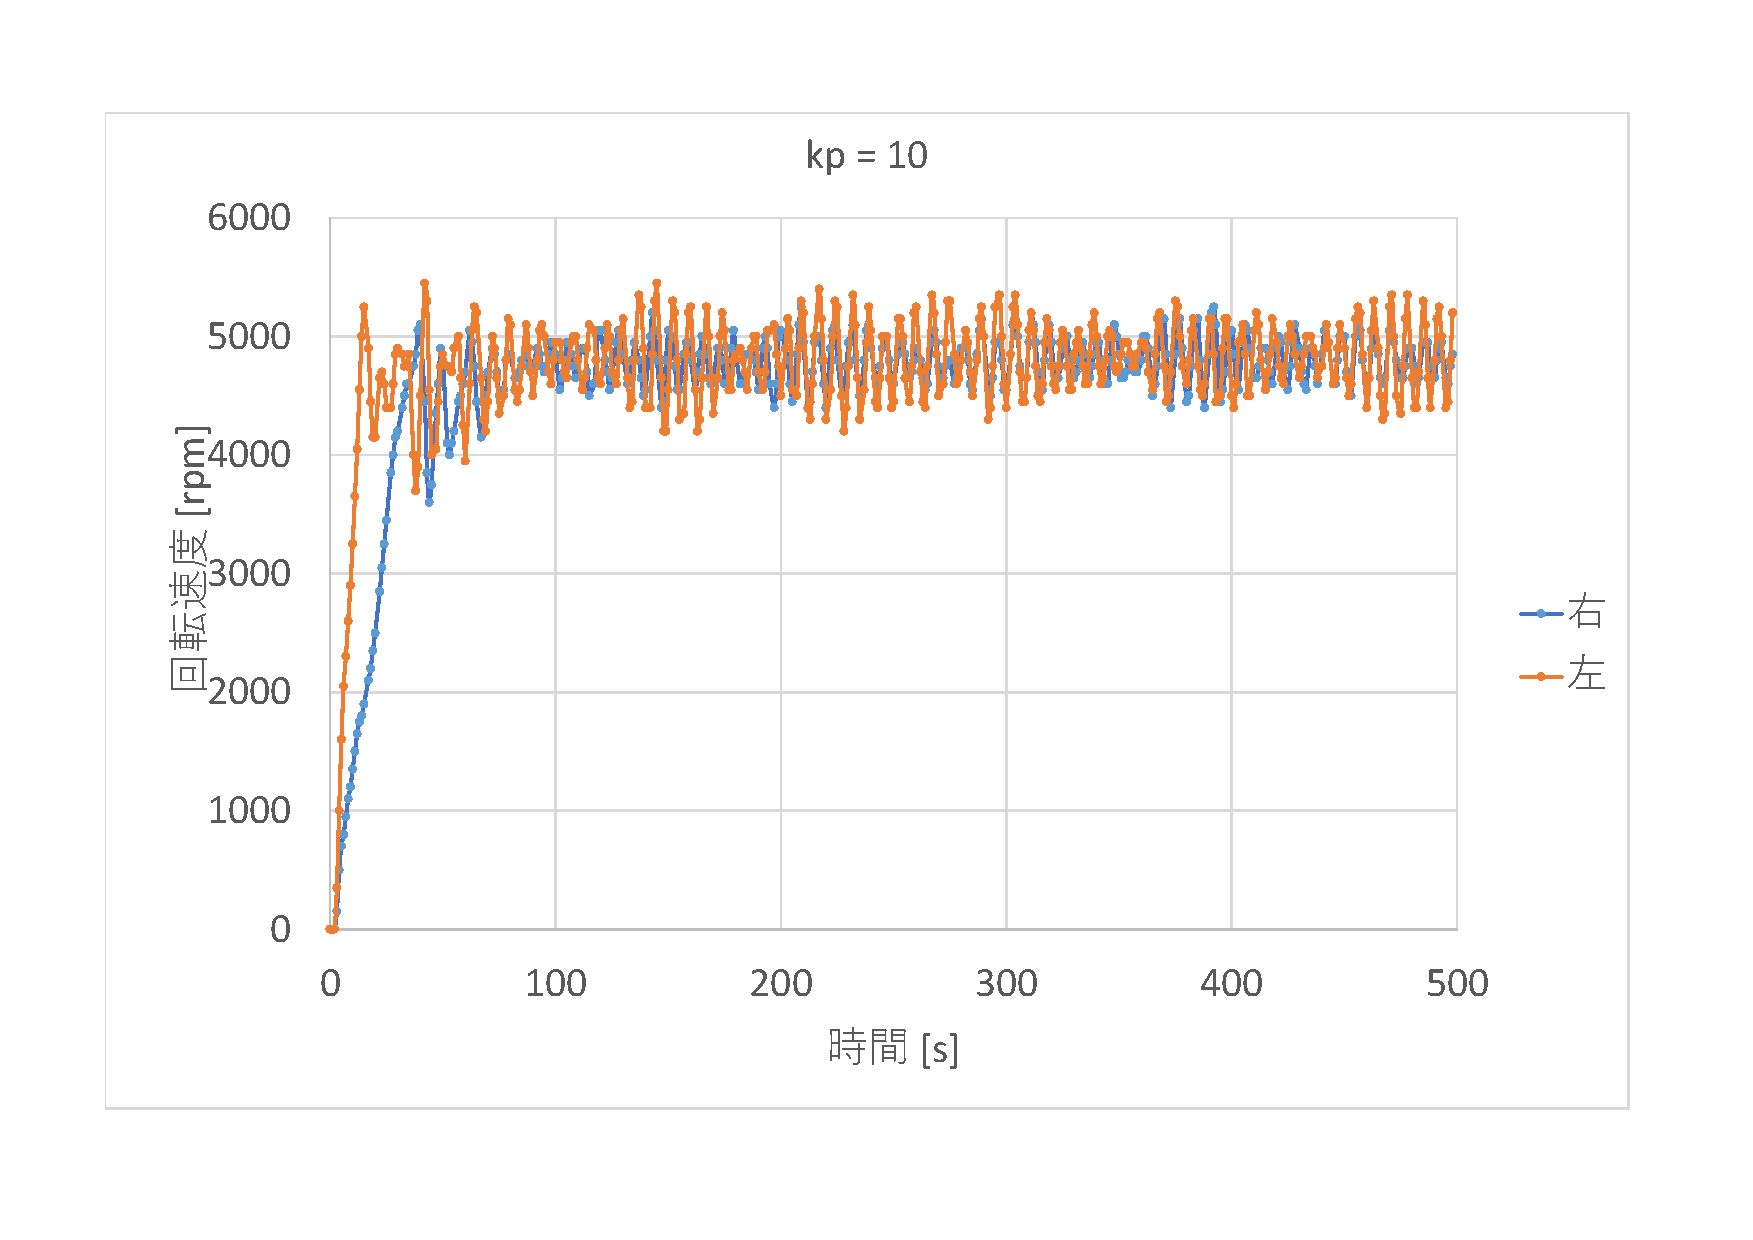
\includegraphics[width=\columnwidth]{img/13/DATA10.pdf}
  \label{im10}
  }
  \subfigure[$k_p=11$]{
  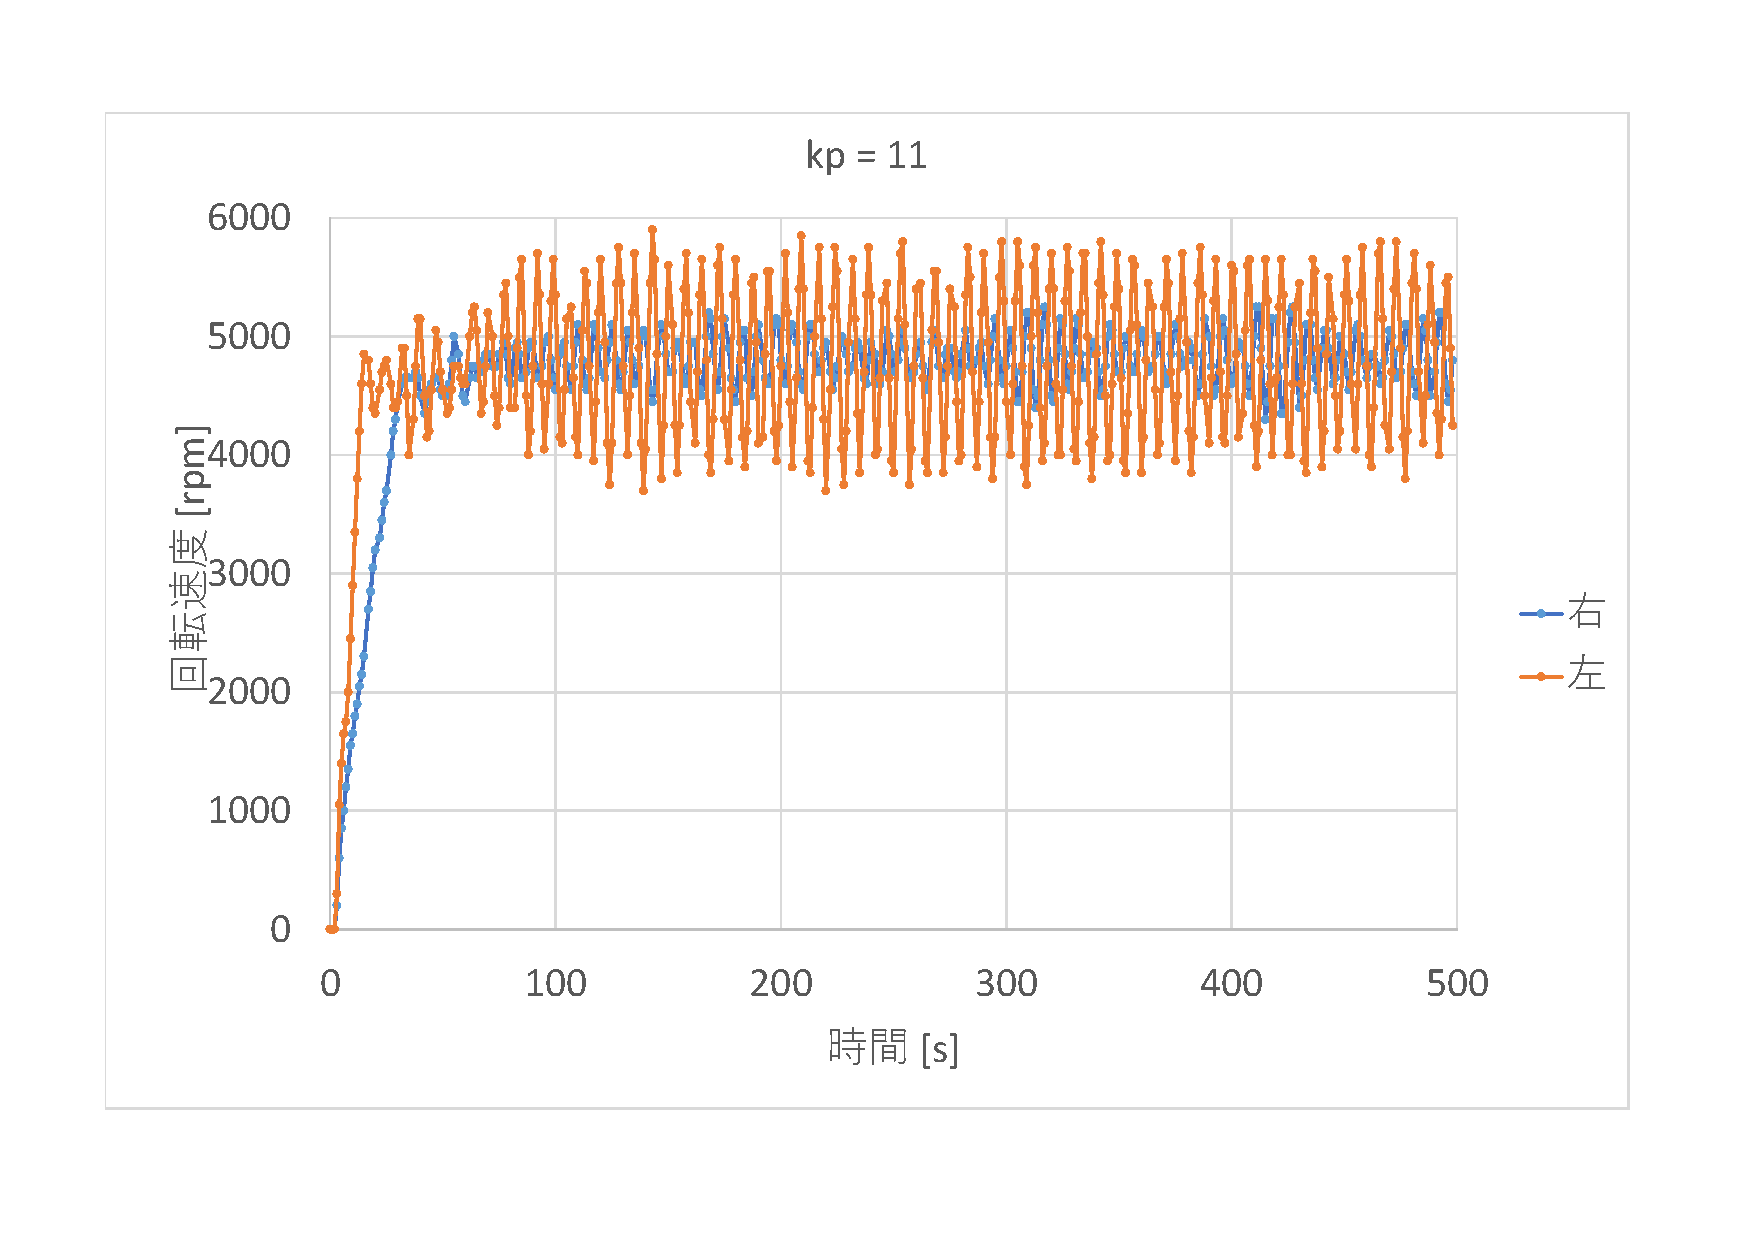
\includegraphics[width=\columnwidth]{img/13/DATA11.pdf}
  \label{im11}
  }
  \caption{ステップ応答のグラフ}
  \end{center}
\end{figure}

\begin{figure}[H]
  \begin{center}
  \subfigure[$k_p=12$]{
  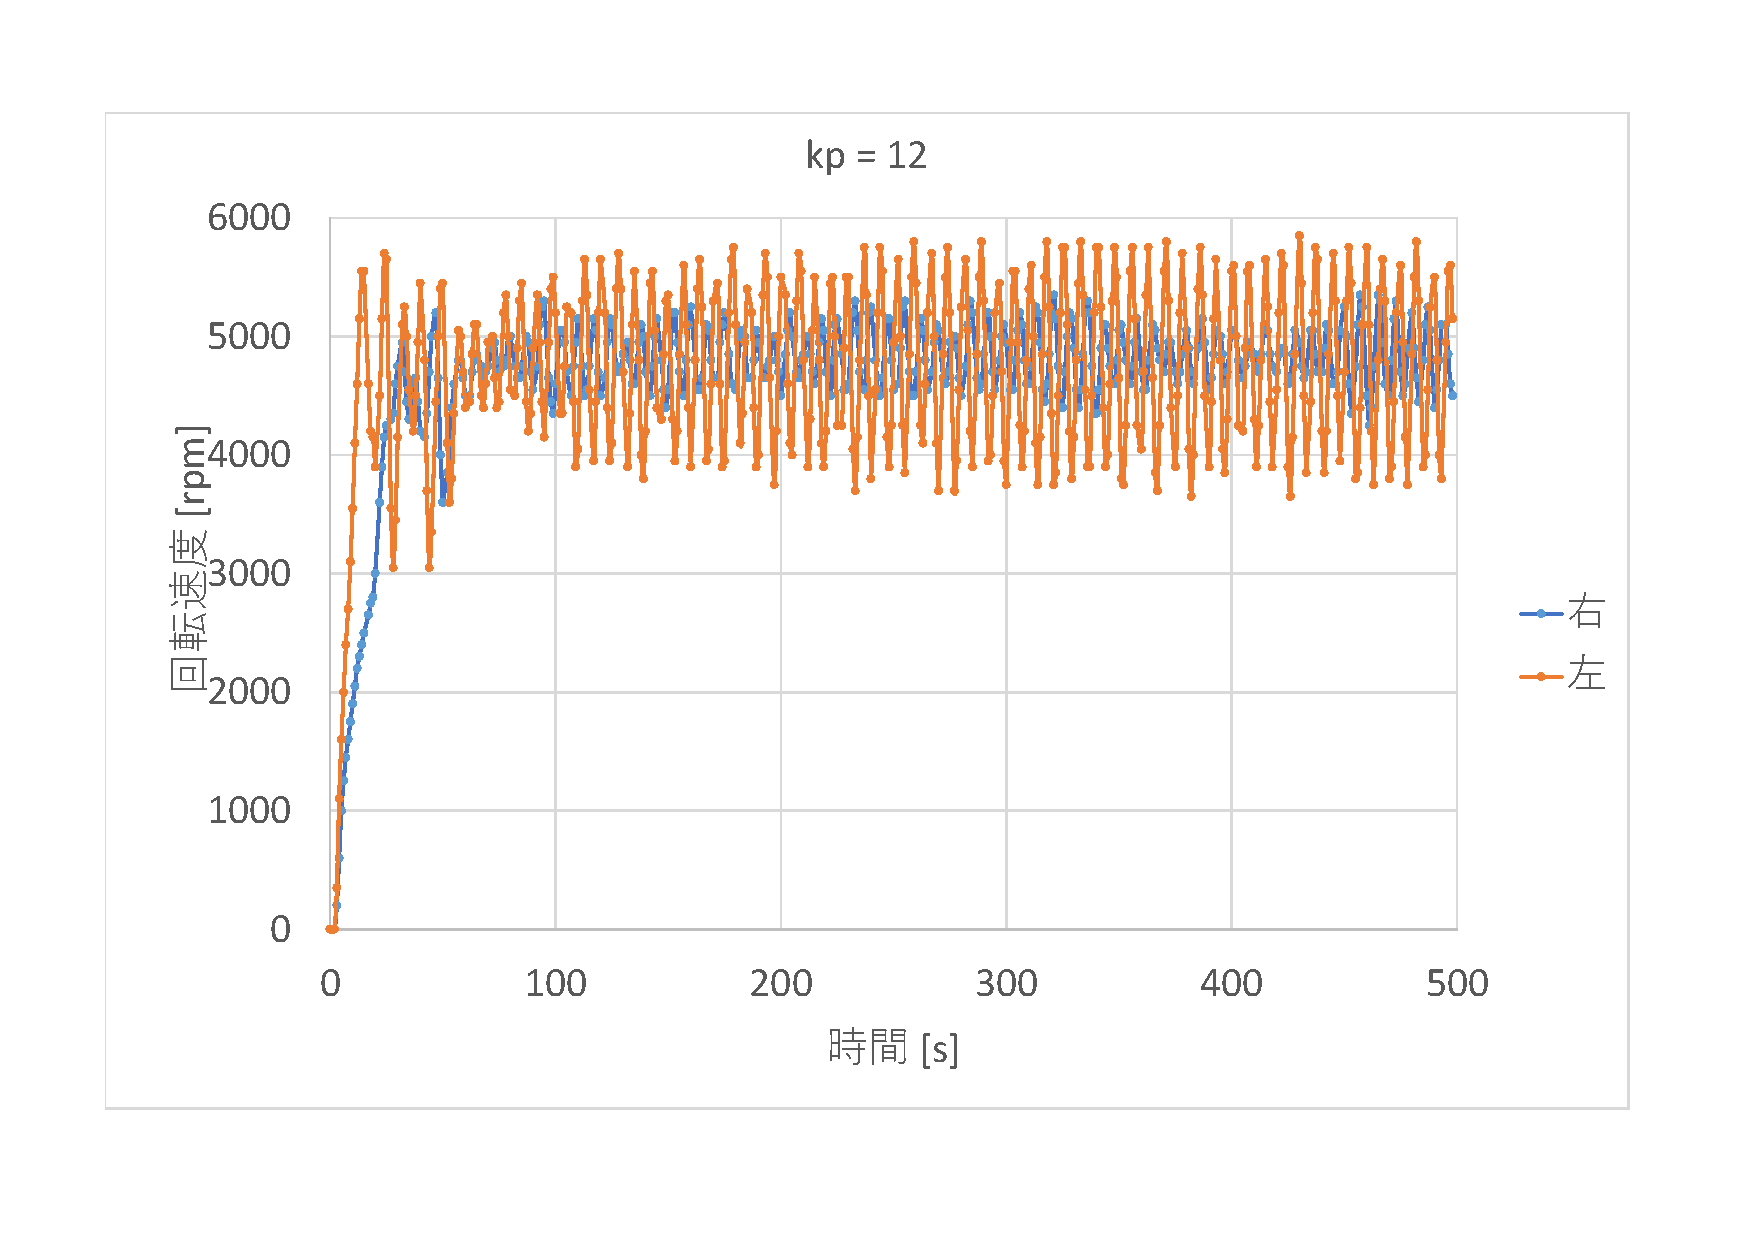
\includegraphics[width=\columnwidth]{img/13/DATA12.pdf}
  \label{im12}
  }
  \subfigure[$k_p=13$]{
  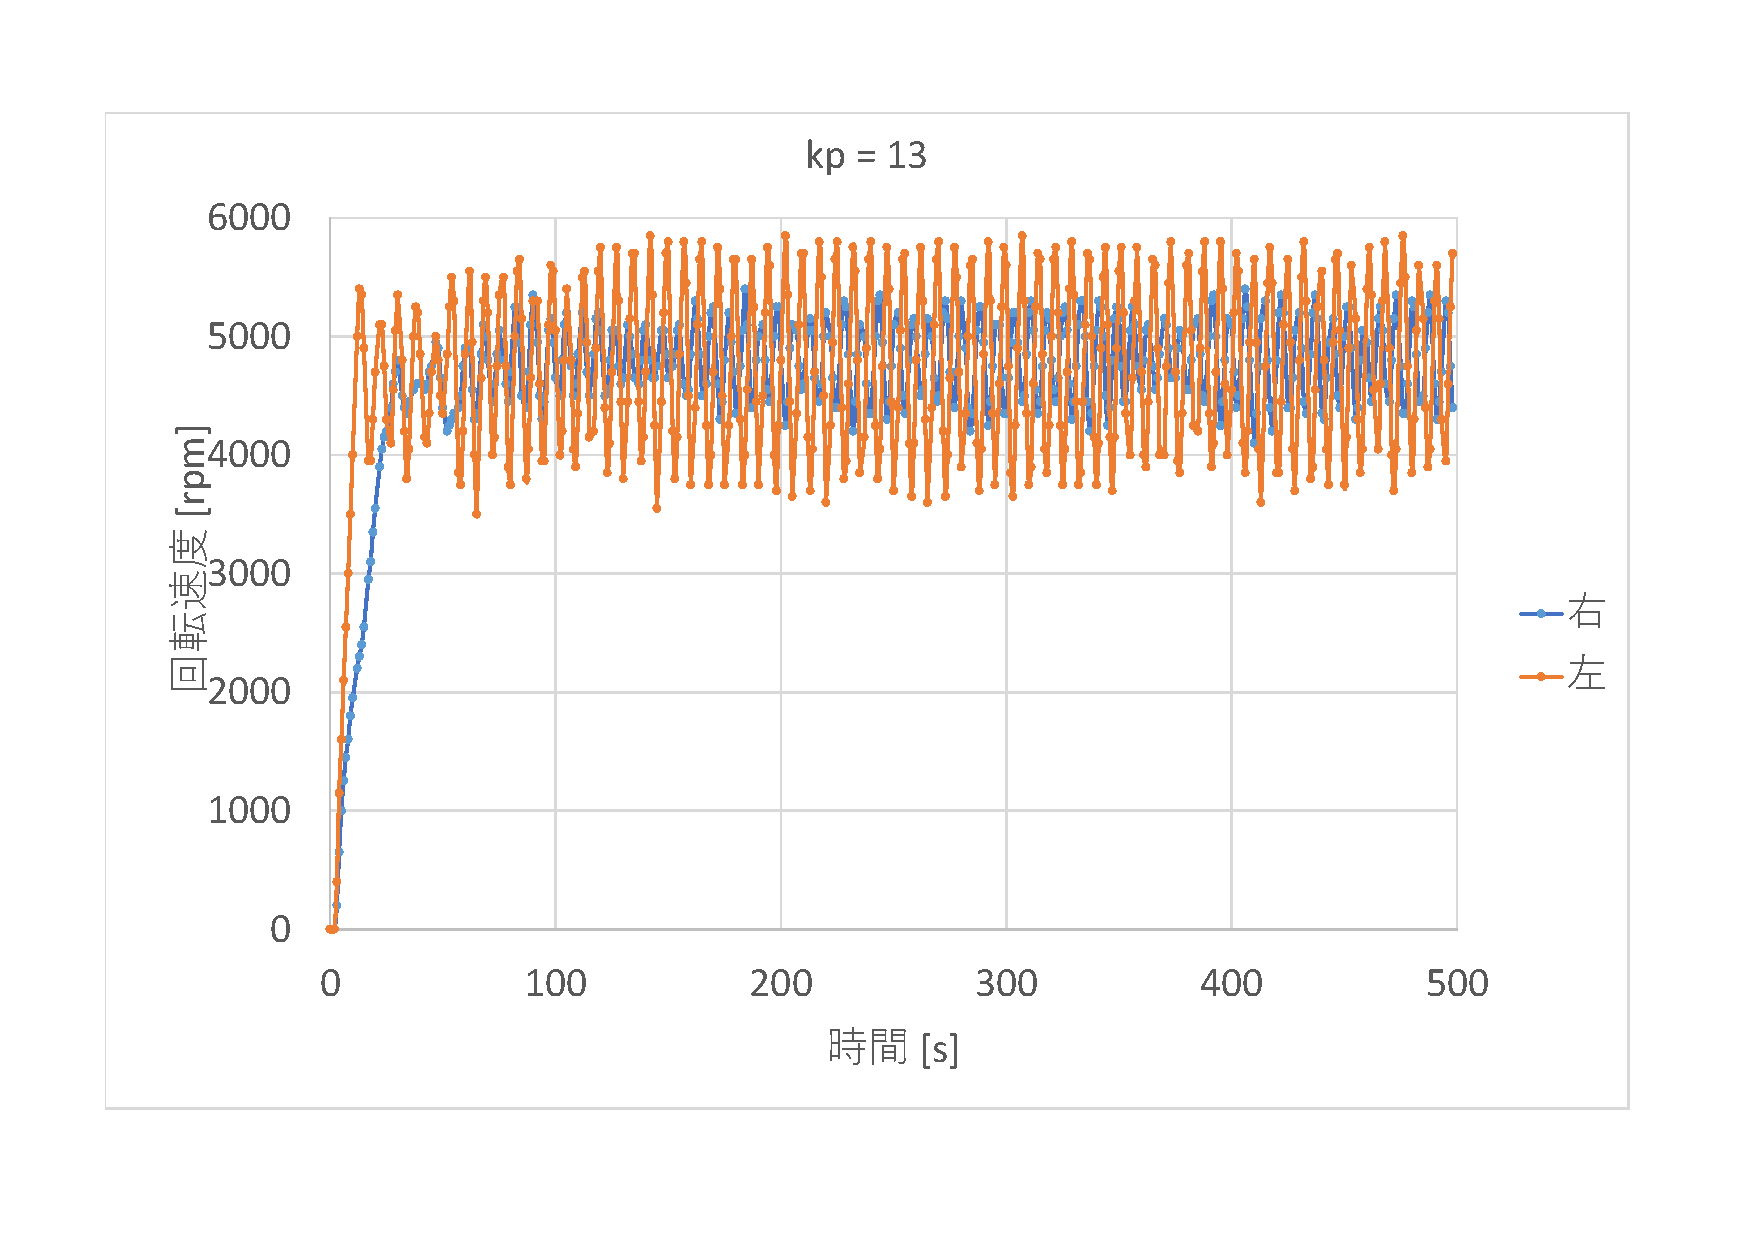
\includegraphics[width=\columnwidth]{img/13/DATA13.pdf}
  \label{im13}
  }
  \caption{ステップ応答のグラフ}
  \end{center}
\end{figure}
\begin{figure}[H]
  \begin{center}
  \subfigure[$k_p=14$]{
  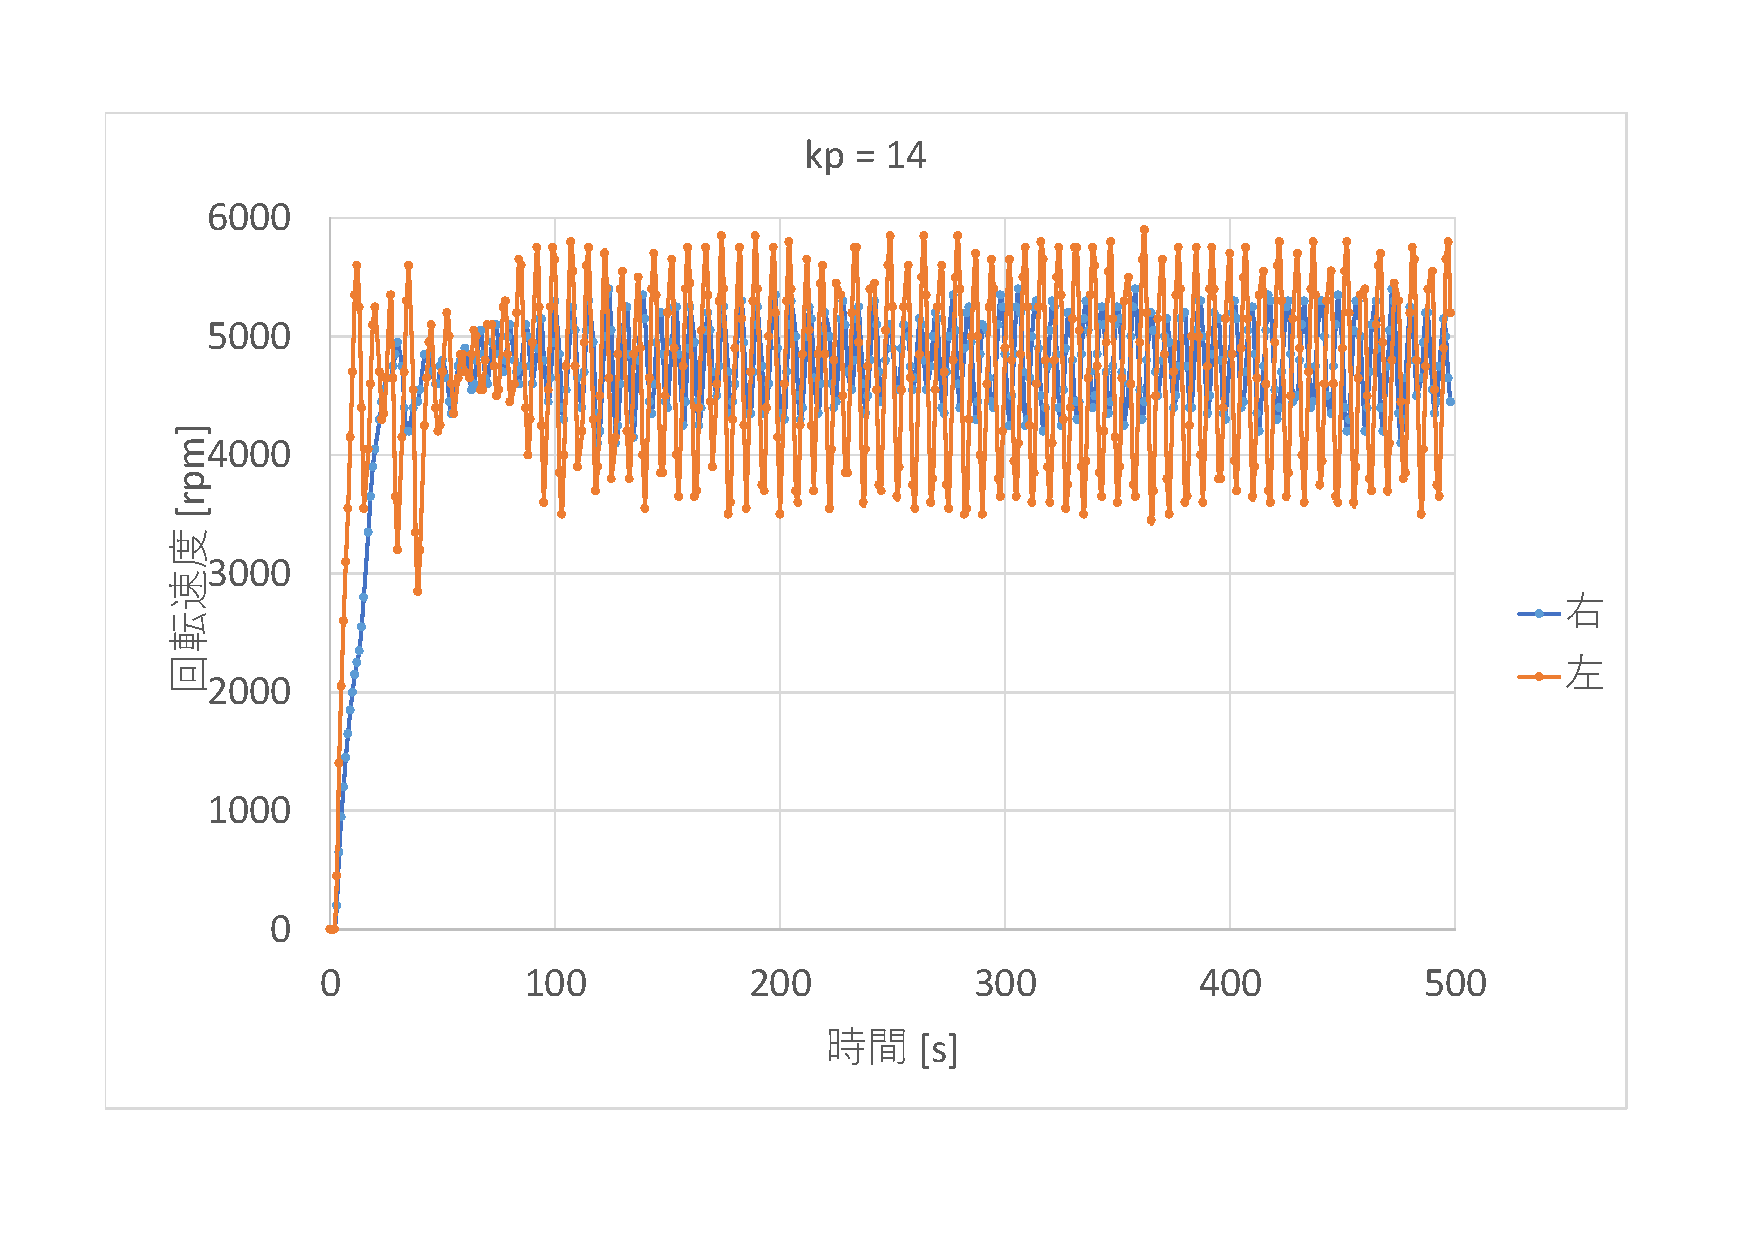
\includegraphics[width=\columnwidth]{img/13/DATA14.pdf}
  \label{im14}
  }
  \subfigure[$k_p=15$]{
  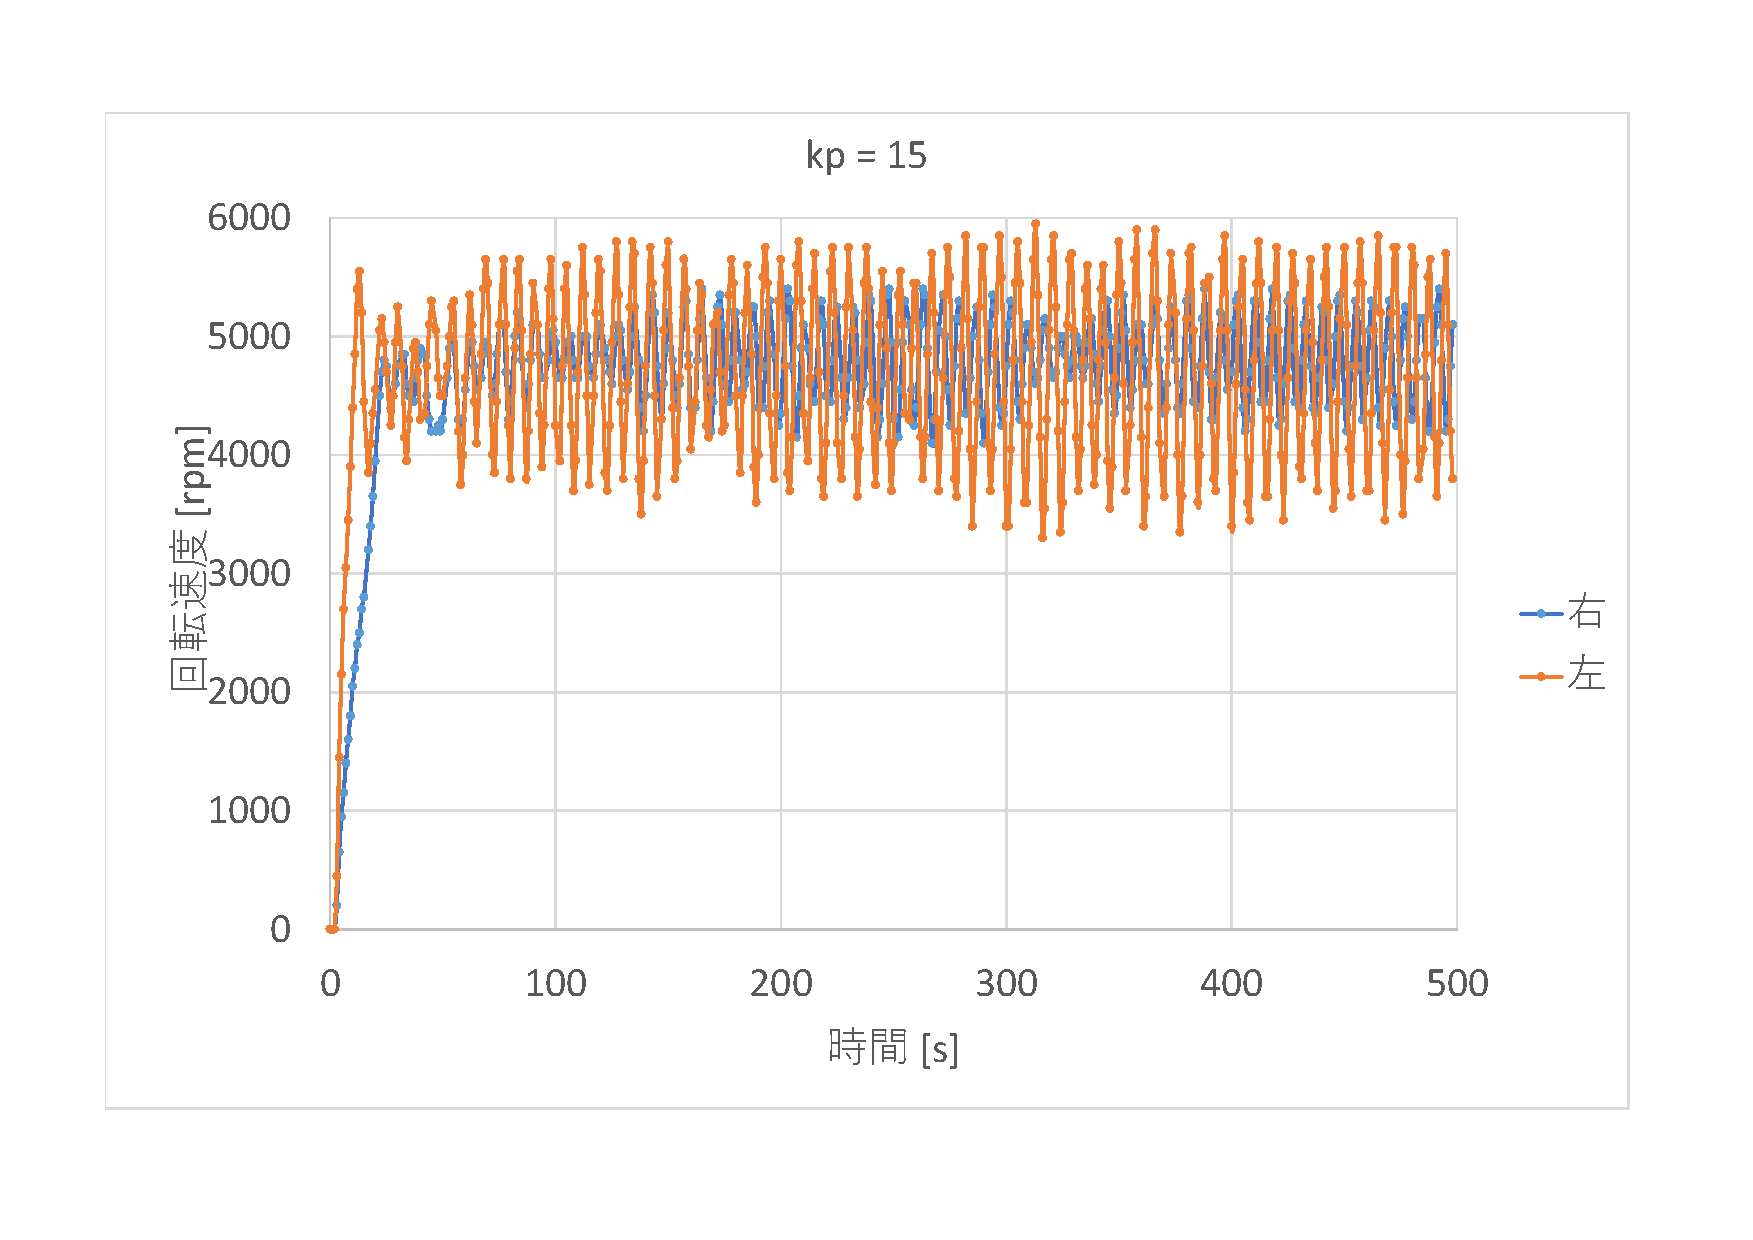
\includegraphics[width=\columnwidth]{img/13/DATA15.pdf}
  \label{im15}
  }
  \caption{ステップ応答のグラフ}
  \end{center}
\end{figure}

\section{演習14}
\subsection{実行プログラム}
実行プログラムをソースコード\ref{s14}に示す。
積分フィードバック係数\verb|ki_inv|$=$\verb|ms_read_dip()*1000|とした。

\begin{lstlisting}[caption=演習14のプログラム,label=s14]
#include <stdio.h>
#include <process.h>
#include <dos.h>
#include "v25.h"
#include "ms.h"
 
#define DMAX 500
  
int main(){
    int i;
    int kp, ki_inv;
    int vrefl, vrefr;
    int vl[DMAX], vr[DMAX];
    long ct, ctm, t[DMAX];
    FILE *fp;
  
    ms_init();
  
    kp = 7;
    ki_inv = ms_read_dip()*1000;
    vrefl = 5000;
    vrefr = 5000;
  
    ms_motor_on();
    ms_read_v(&vl[0], &vr[0], &ctm);
    ms_step_res(vrefl, vrefr, kp, ki_inv);
  for(i=1; i<DMAX; i++){
    ms_read_v(&vl[i], &vr[i], &ct);
    t[i] = ct - ctm;
    ms_wait(2);
  }
  ms_motor_off();
  
  if((fp = fopen("data.dat", "wt")) == NULL){
    printf("Can't Open File!!\n");
    exit(1);
  }
  
  for(i=1; i<DMAX; i++){
    fprintf(fp, "%7d %7d %10ld\n", vl[i], vr[i], t[i]);
  }
  fclose(fp);
  ms_beep(440,500);
  printf("owari\n");
  return 0;
}
\end{lstlisting}

\subsection{実行結果}
演習13と同様に
モータのステップ応答(回転速度と時間)
をデータファイルに保存する。
応答グラフを図\ref{im15_14}\verb|~|\ref{im1_14}に示す。
積分フィードバック係数$k_i=1/13000$を最適な値とした。
つまり、\verb|ms_read_dip()|$=$\tsuyo{13}の値である。

\begin{figure}[H]
  \begin{center}
  \subfigure[$k_i=1/15000$]{
  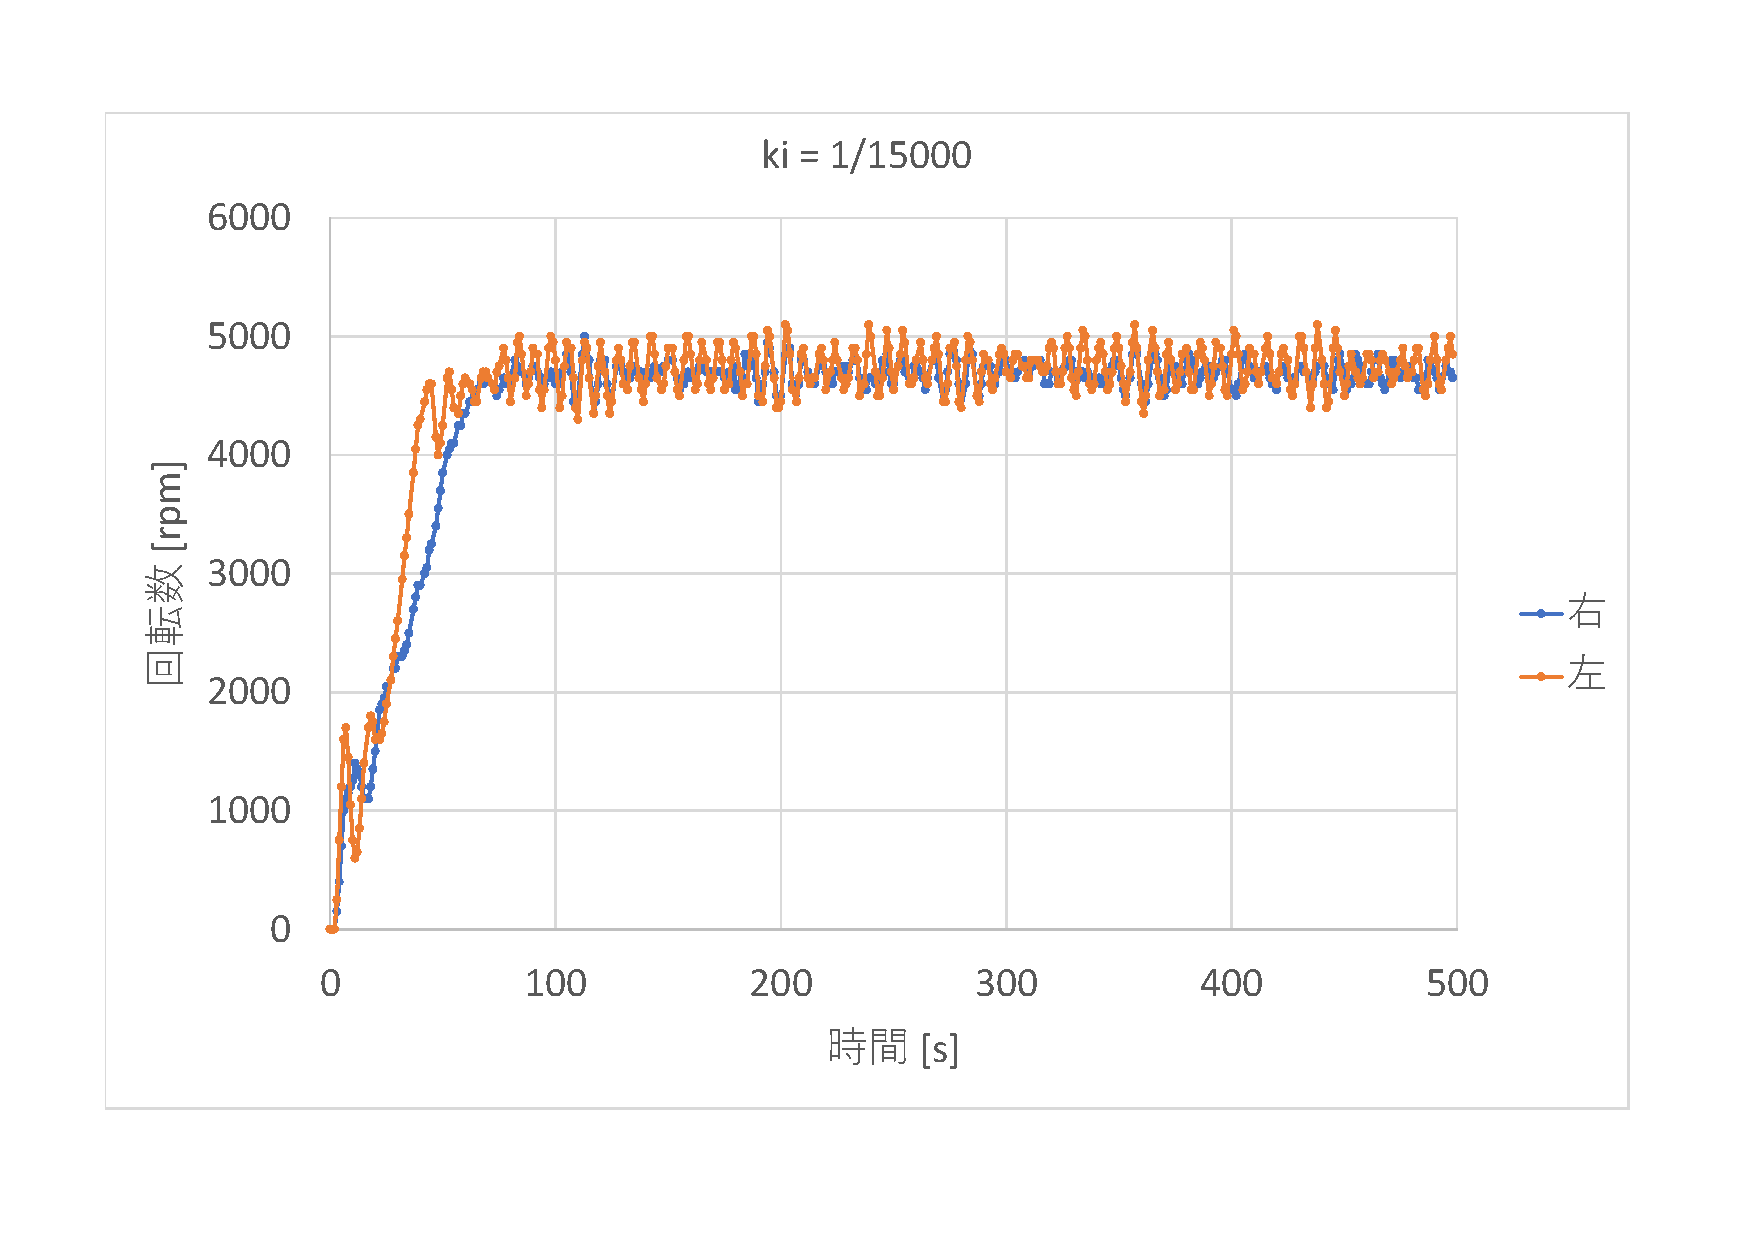
\includegraphics[width=.7\columnwidth]{img/14/DATA15.pdf}
  \label{im15_14}
  }
  \subfigure[$k_i=1/14000$]{
  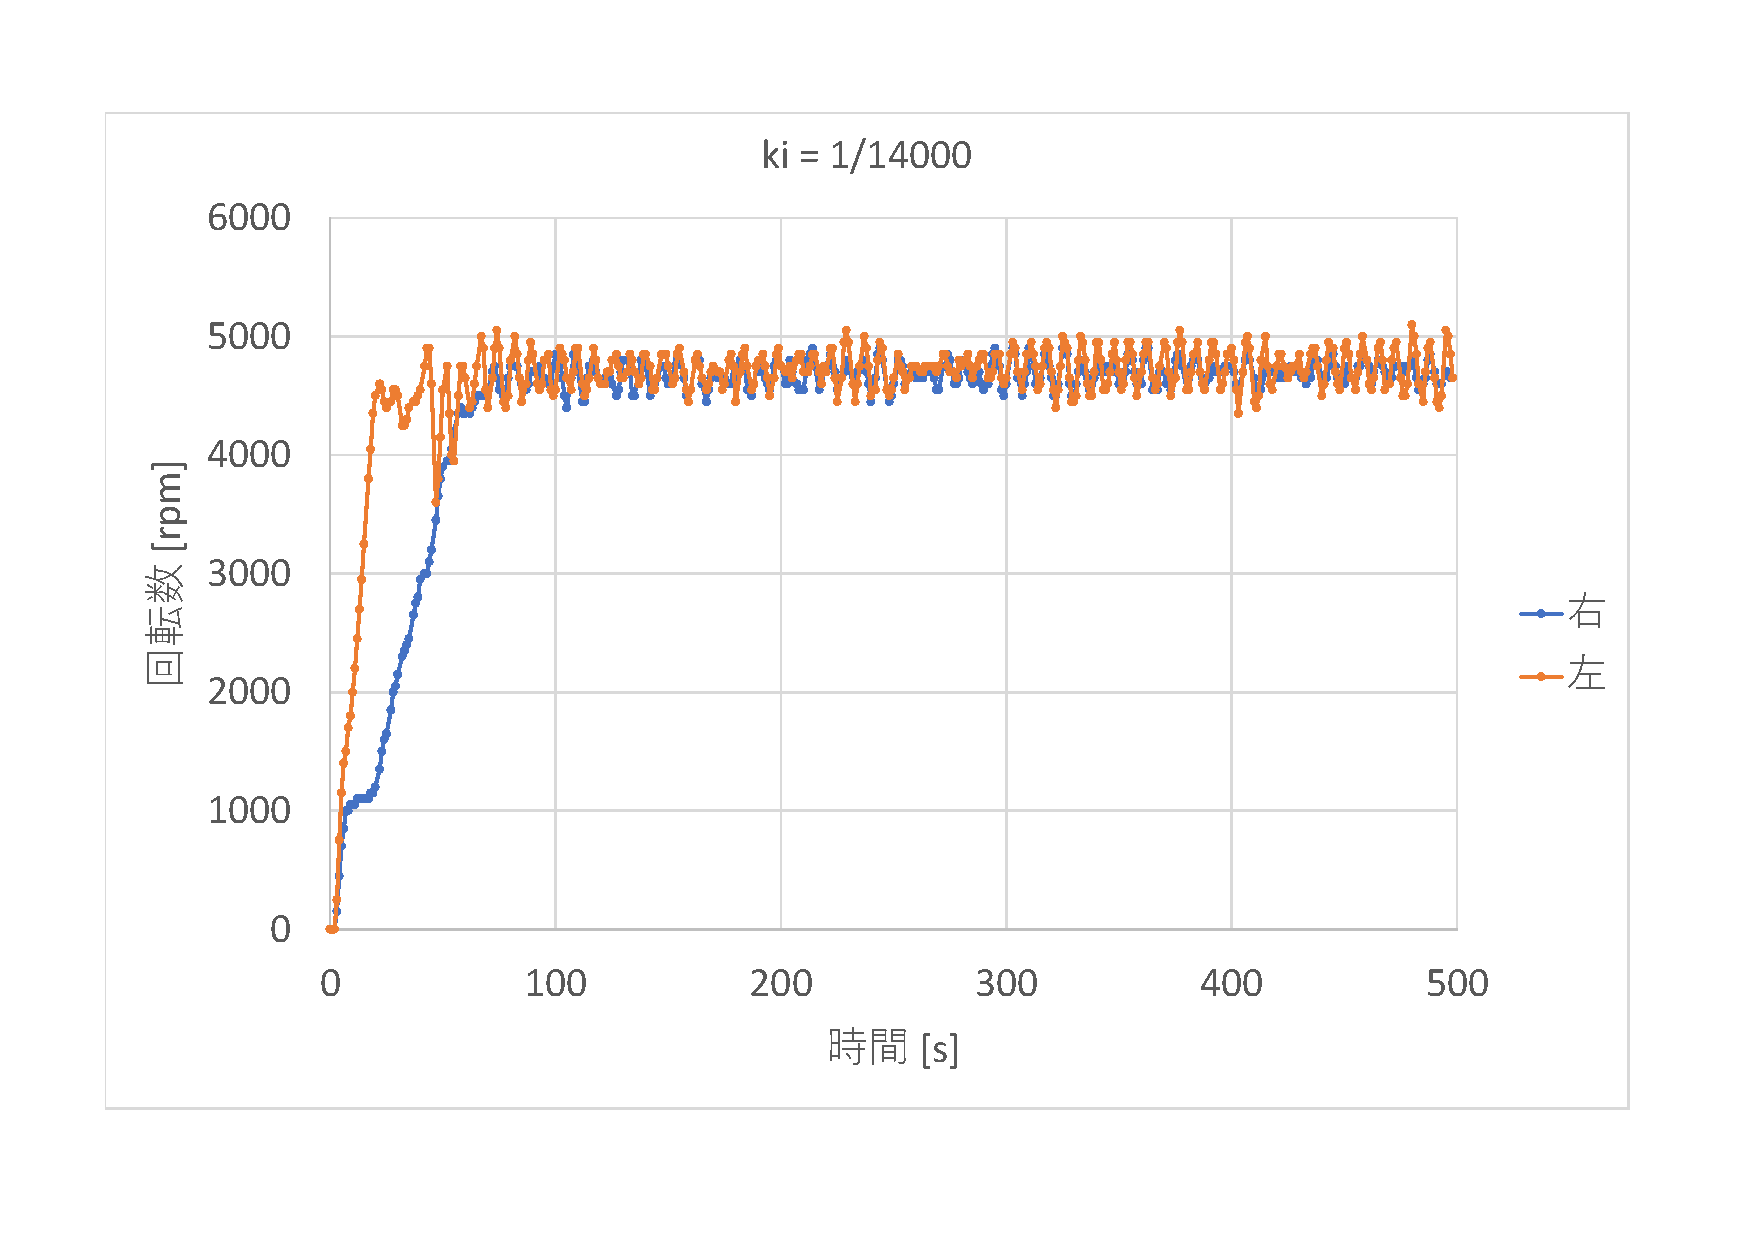
\includegraphics[width=.7\columnwidth]{img/14/DATA14.pdf}
  \label{im14_14}
  }
  \caption{ステップ応答のグラフ}
  \end{center}
\end{figure}
\begin{figure}[H]
  \begin{center}
  \subfigure[$k_i=1/13000$]{
  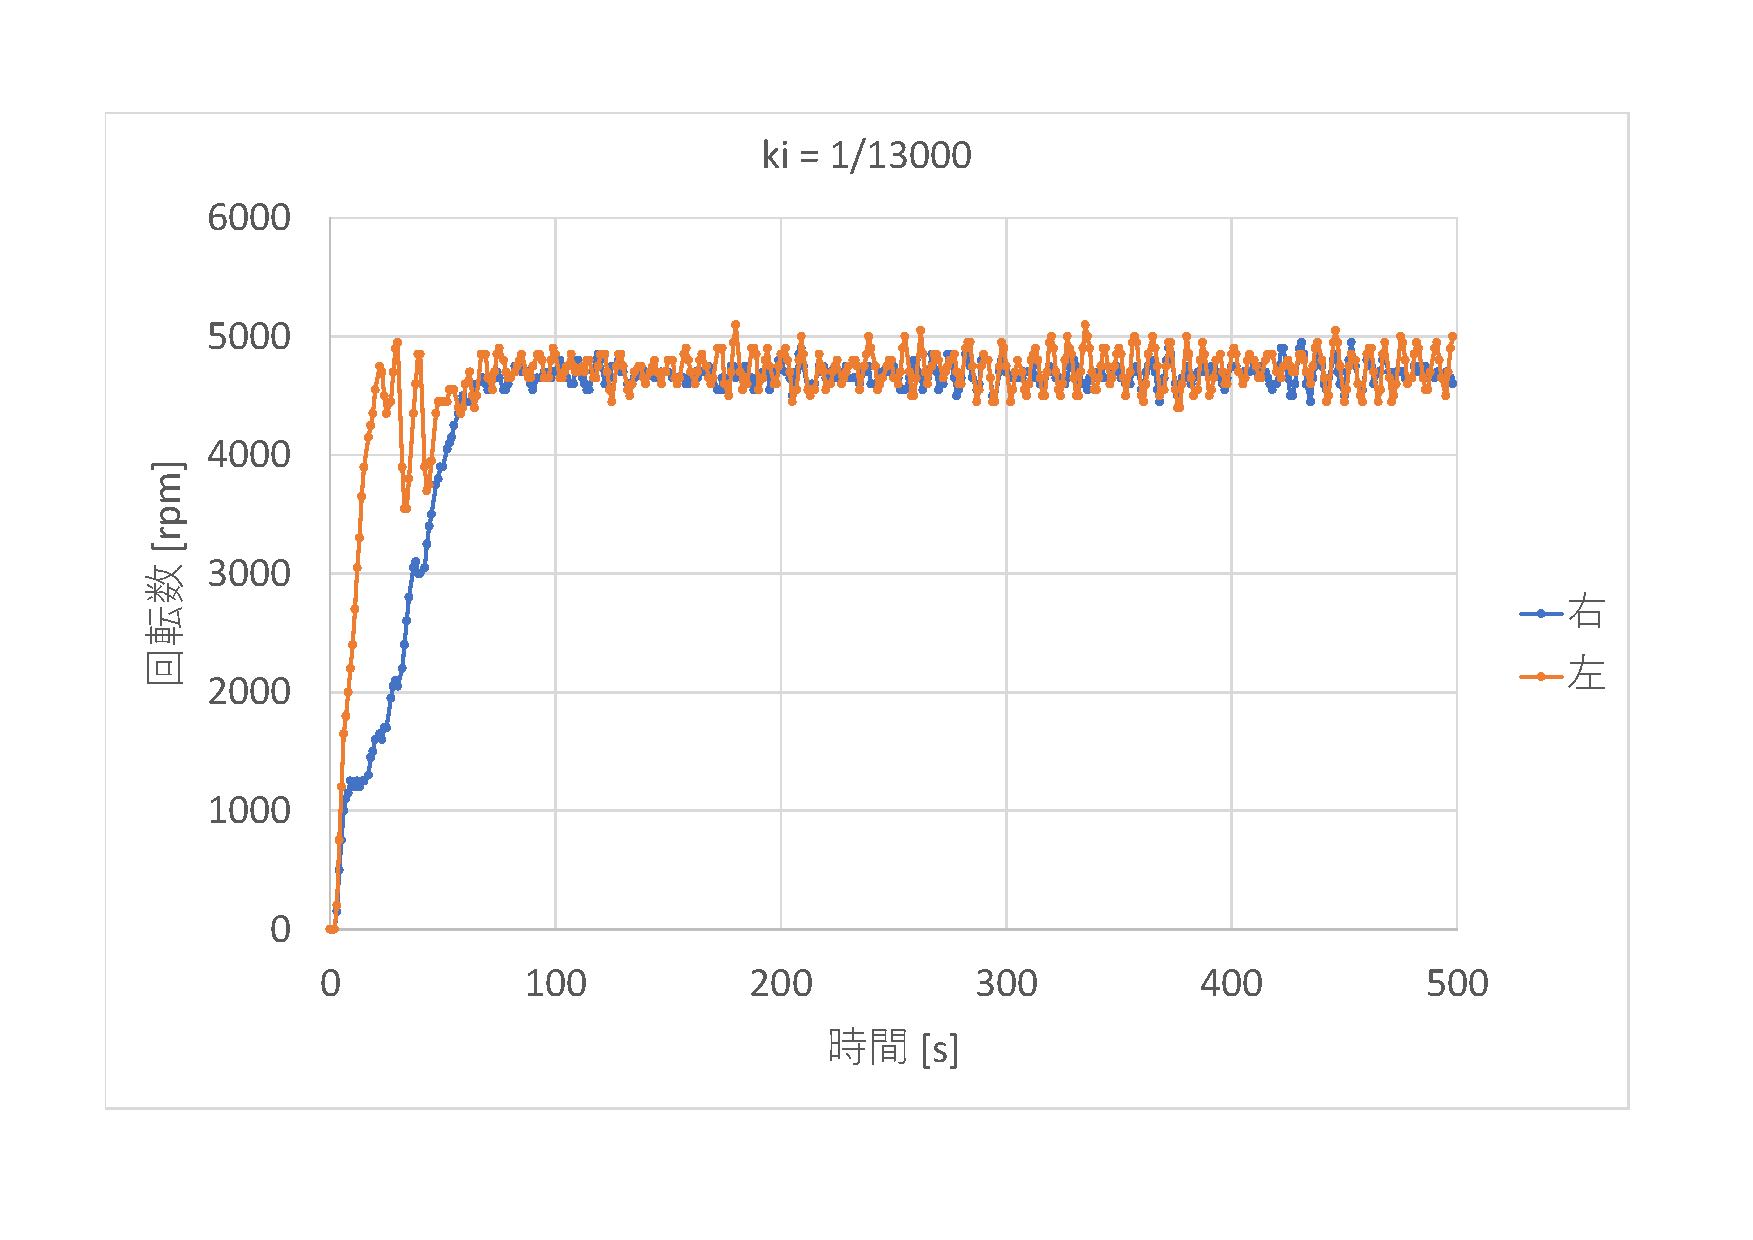
\includegraphics[width=\columnwidth]{img/14/DATA13.pdf}
  \label{im13_14}
  }
  \subfigure[$k_i=1/12000$]{
  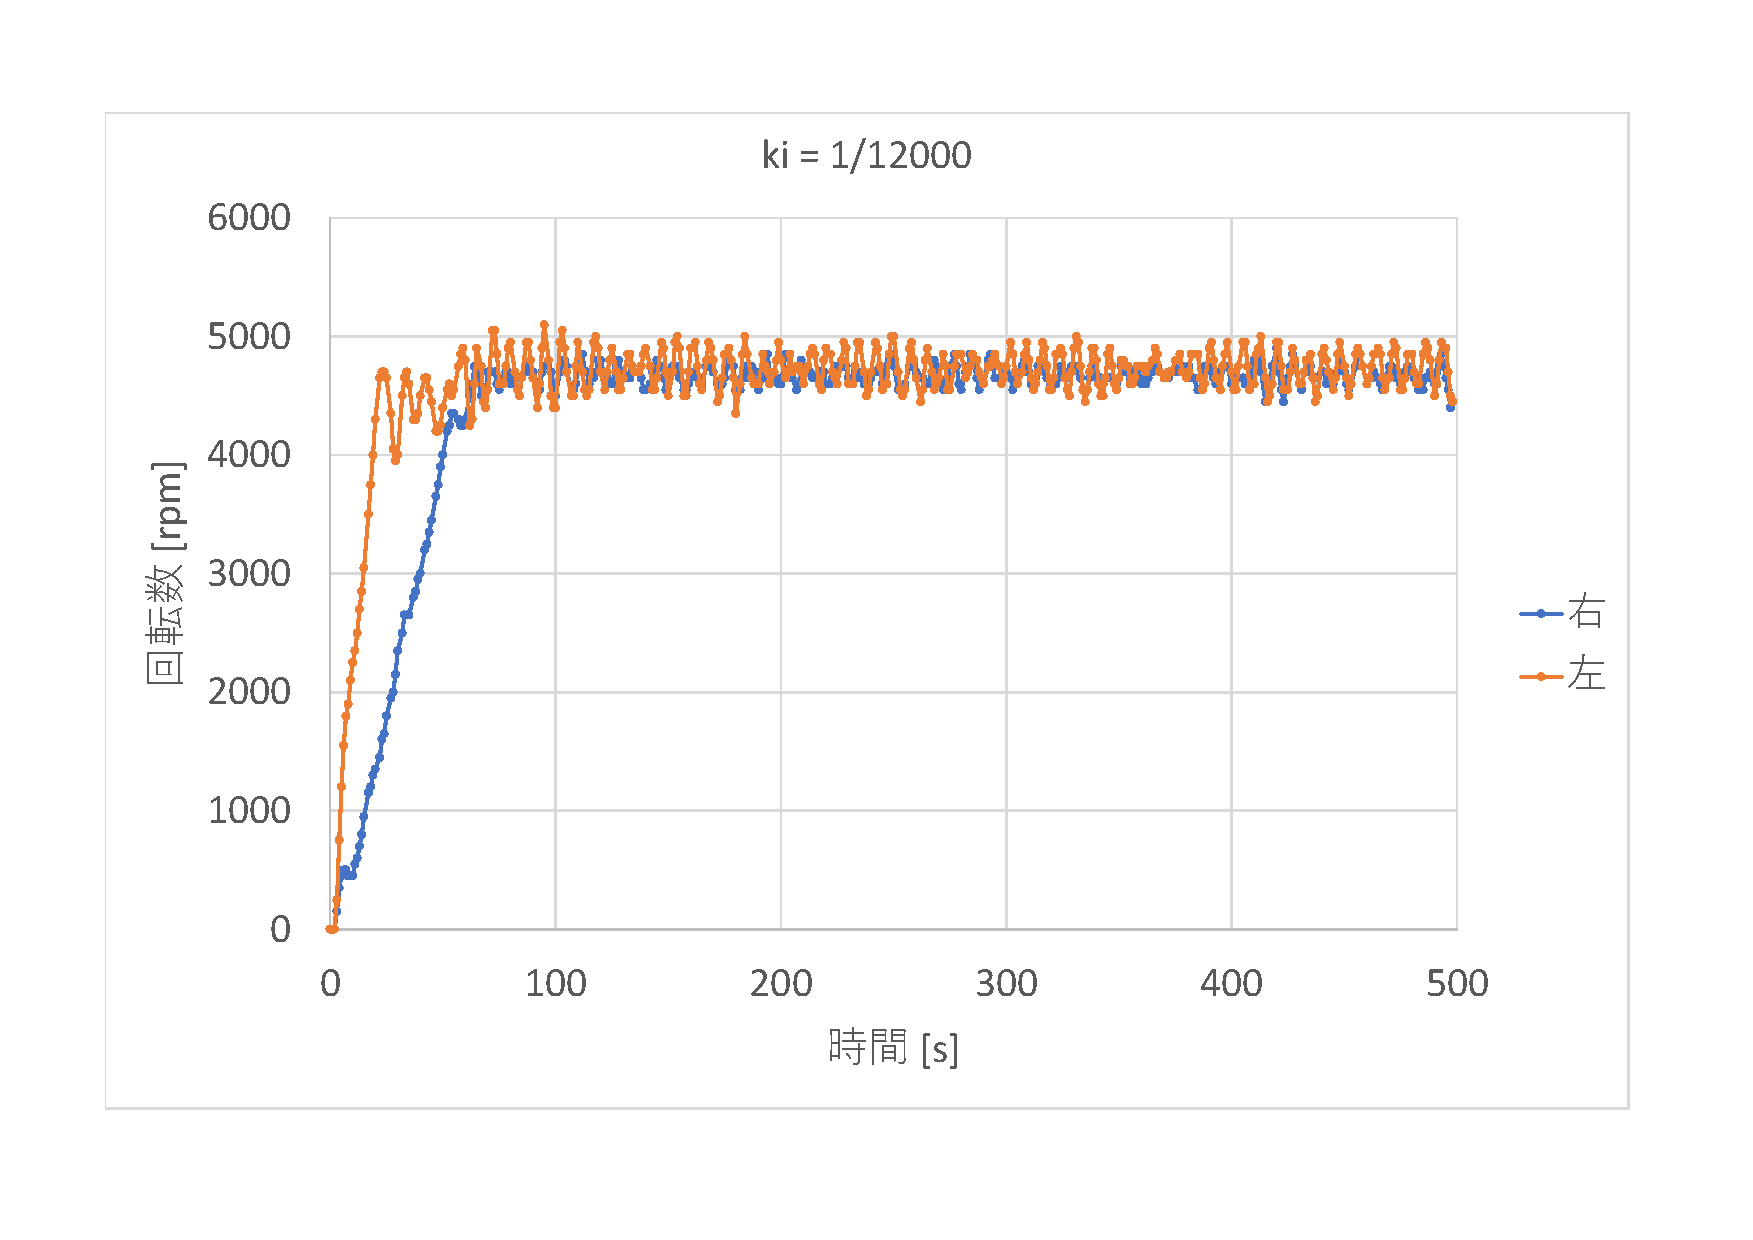
\includegraphics[width=\columnwidth]{img/14/DATA12.pdf}
  \label{im12_14}
  }
  \caption{ステップ応答のグラフ}
  \end{center}
\end{figure}
\begin{figure}[H]
  \begin{center}
  \subfigure[$k_i=1/11000$]{
  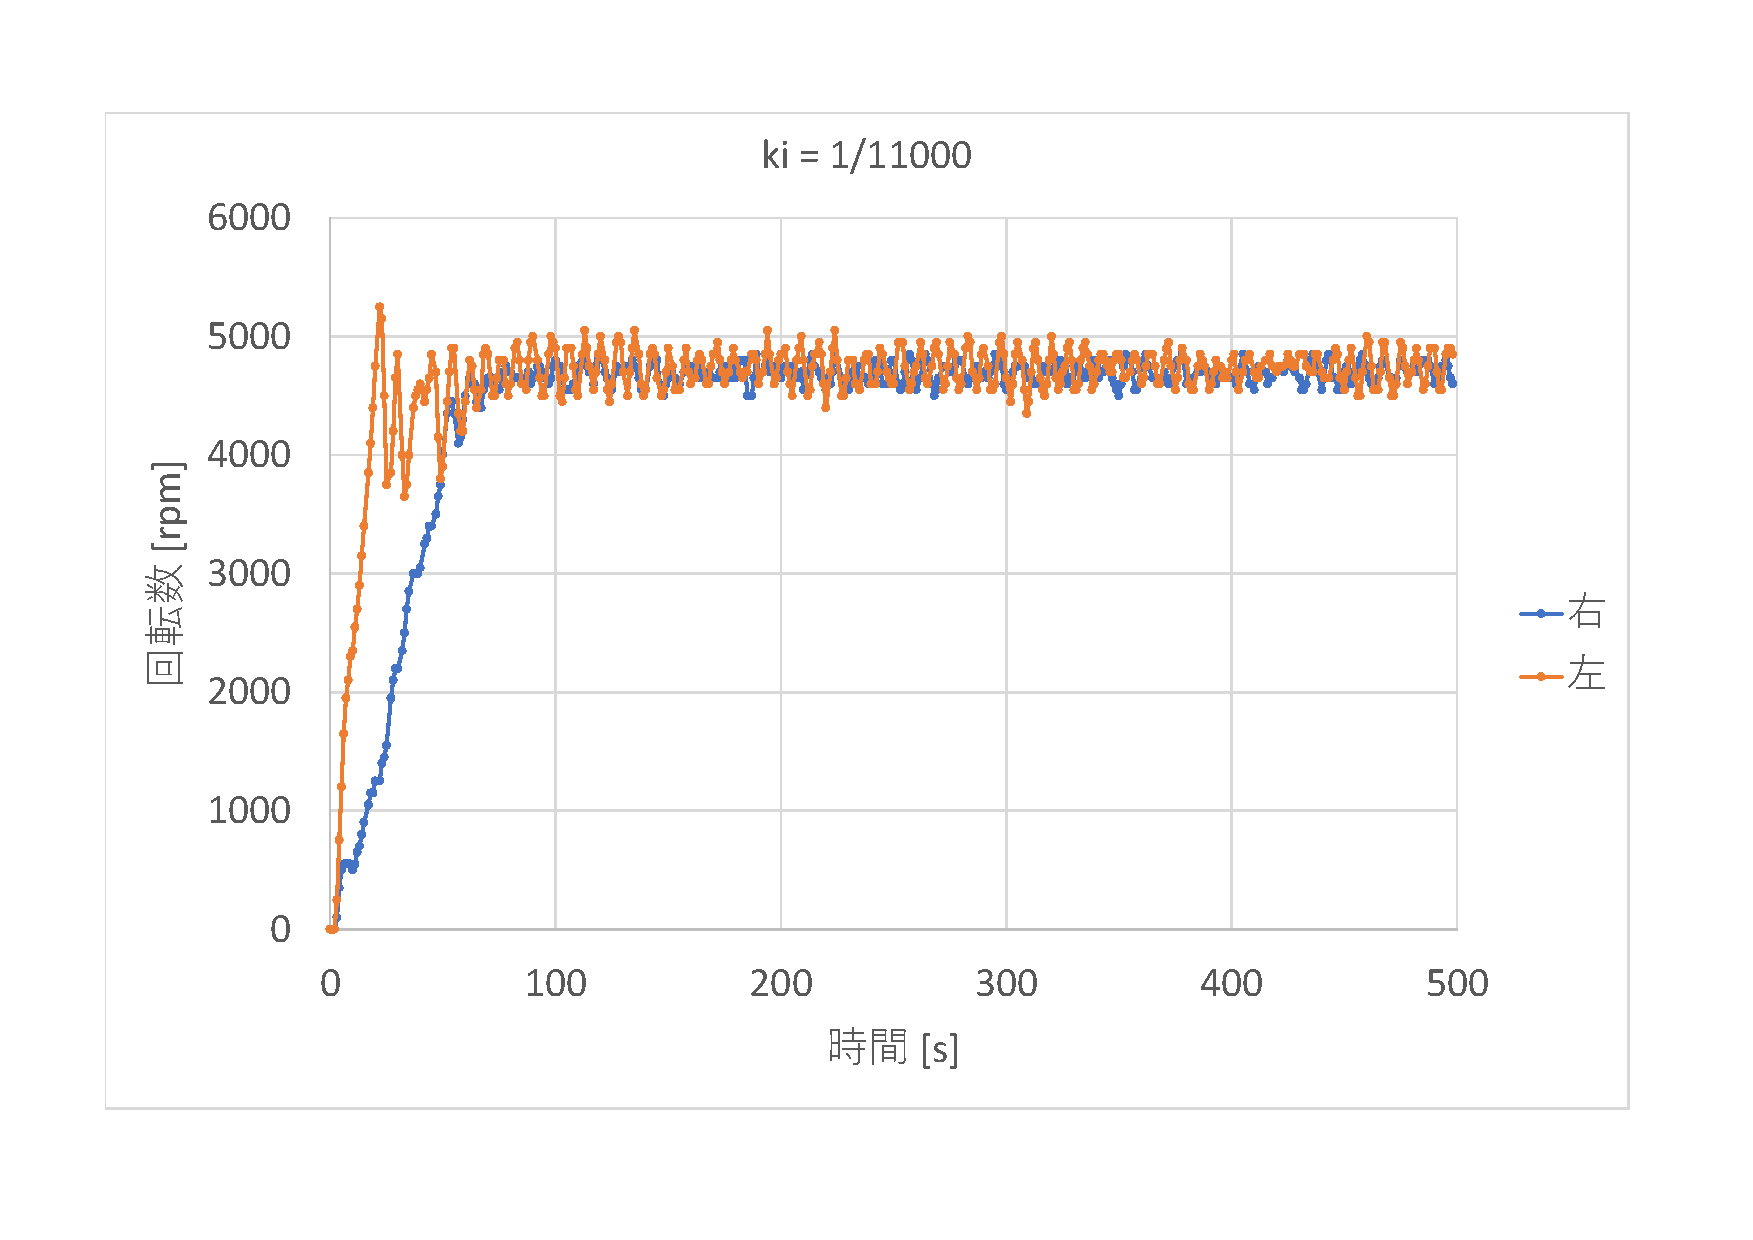
\includegraphics[width=\columnwidth]{img/14/DATA11.pdf}
  \label{im11_14}
  }
  \subfigure[$k_i=1/10000$]{
  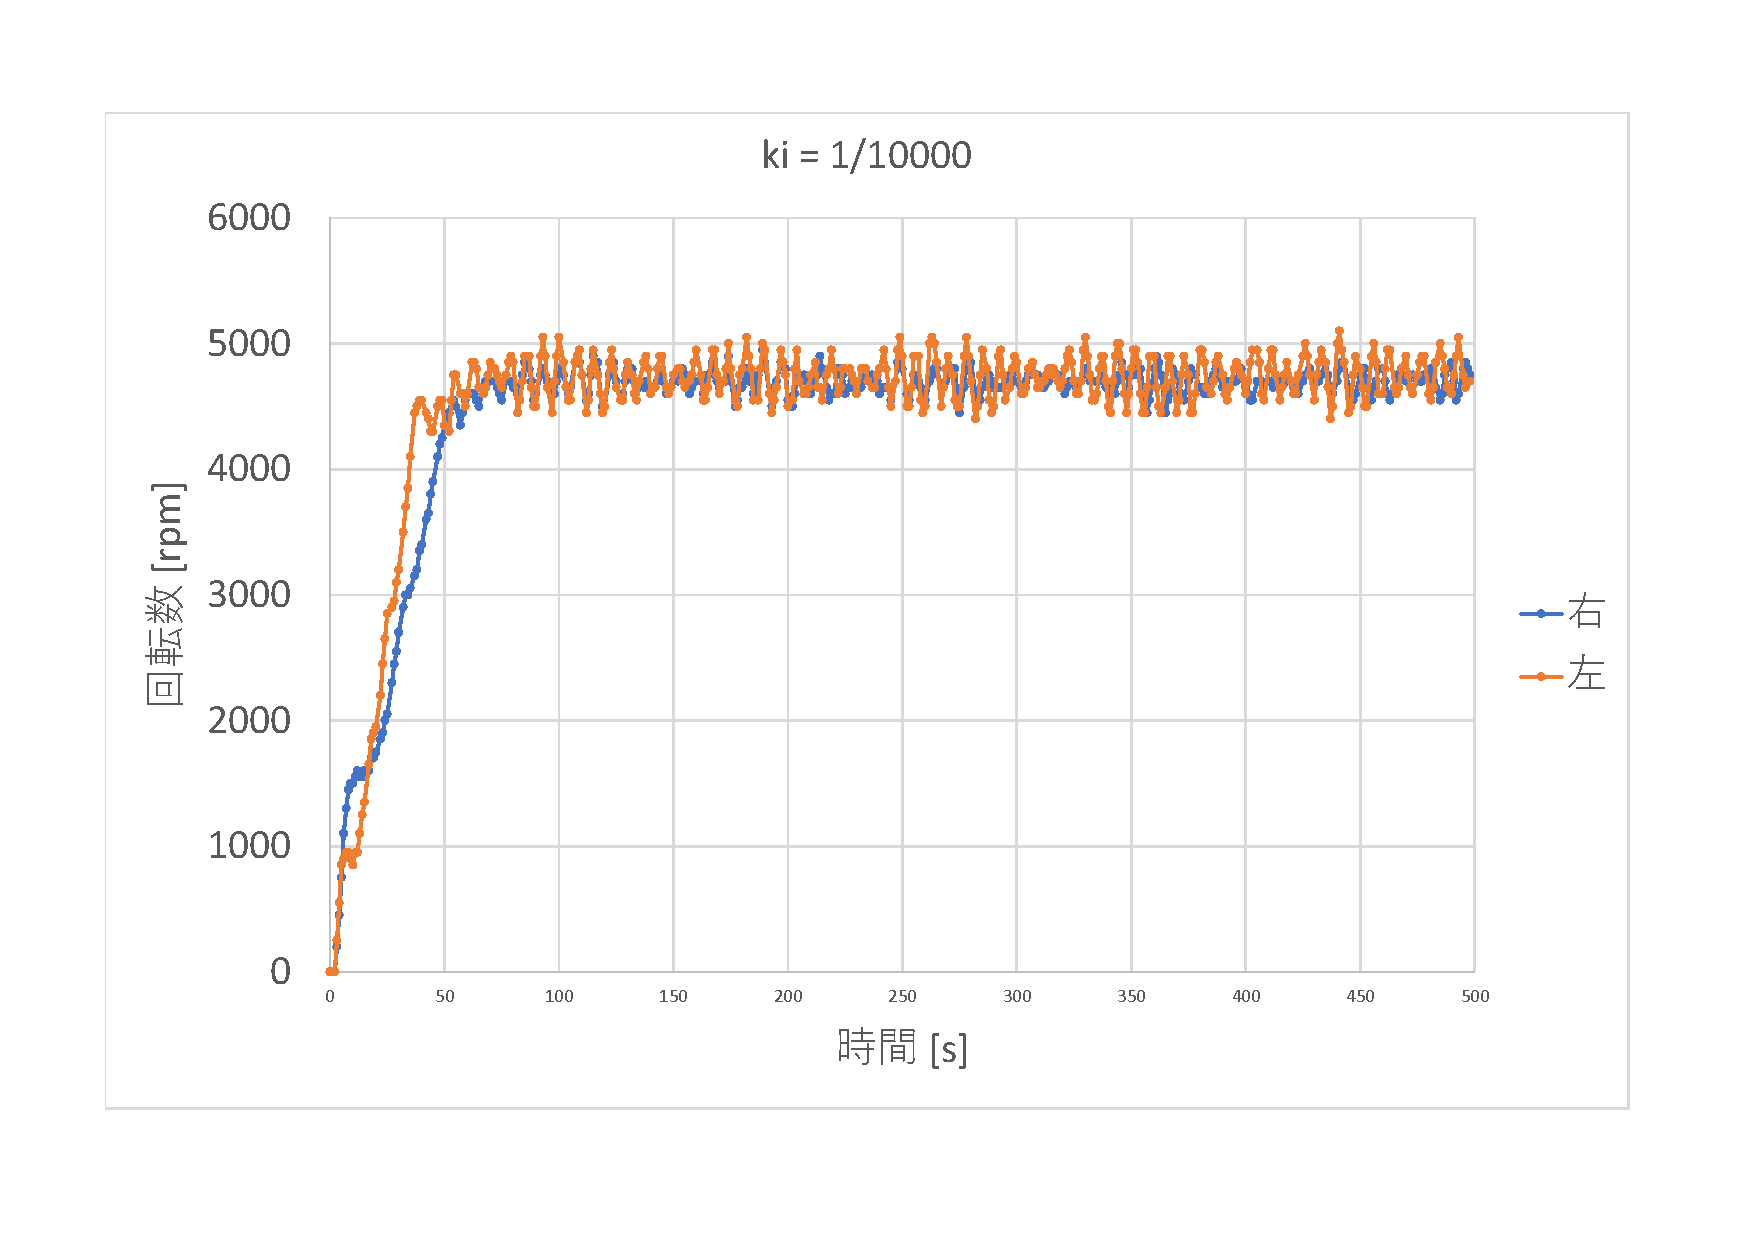
\includegraphics[width=\columnwidth]{img/14/DATA10.pdf}
  \label{im10_14}
  }
  \caption{ステップ応答のグラフ}
  \end{center}
\end{figure}
\begin{figure}[H]
  \begin{center}
  \subfigure[$k_i=1/9000$]{
  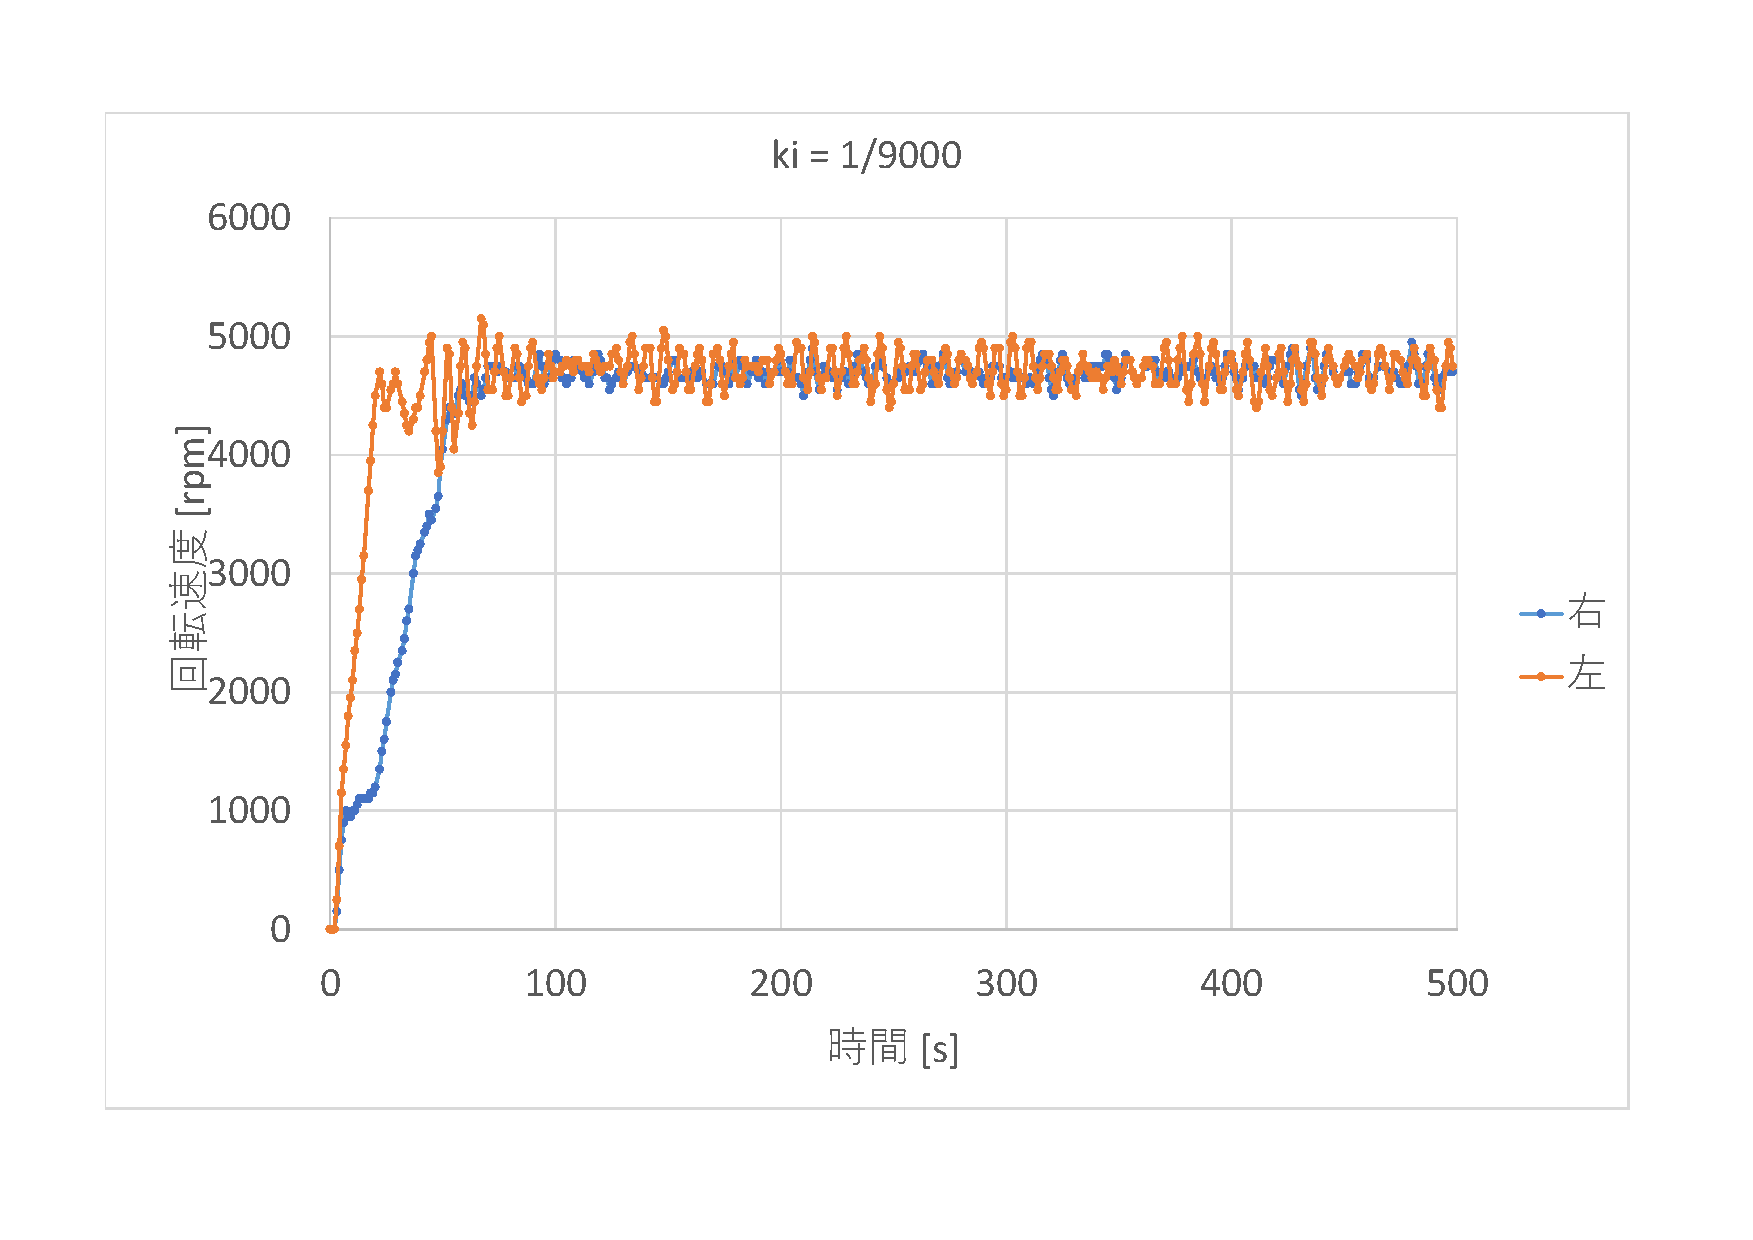
\includegraphics[width=\columnwidth]{img/14/DATA9.pdf}
  \label{im9_14}
  }
  \subfigure[$k_i=1/8000$]{
  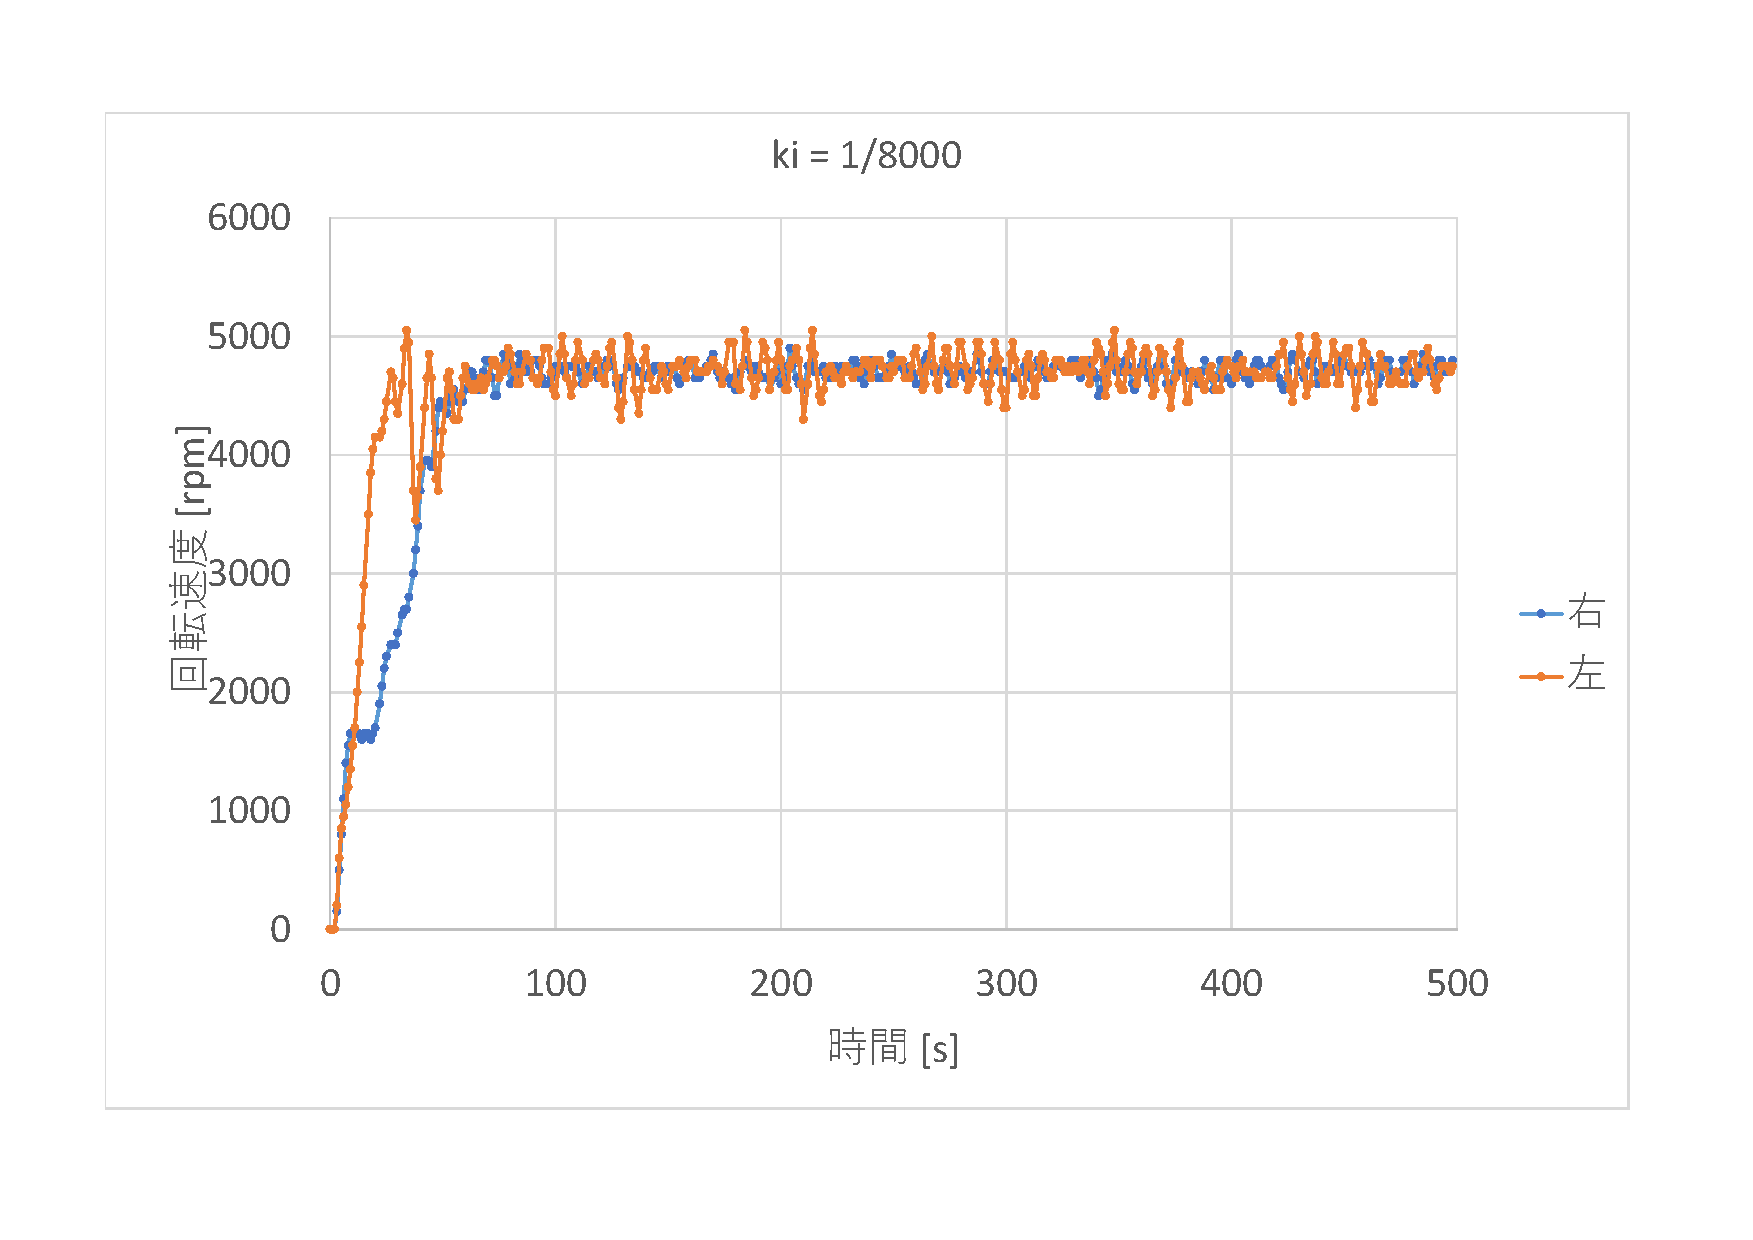
\includegraphics[width=\columnwidth]{img/14/DATA8.pdf}
  \label{im8_14}
  }
  \end{center}
\end{figure}
\begin{figure}[H]
  \begin{center}
  \subfigure[$k_i=1/7000$]{
  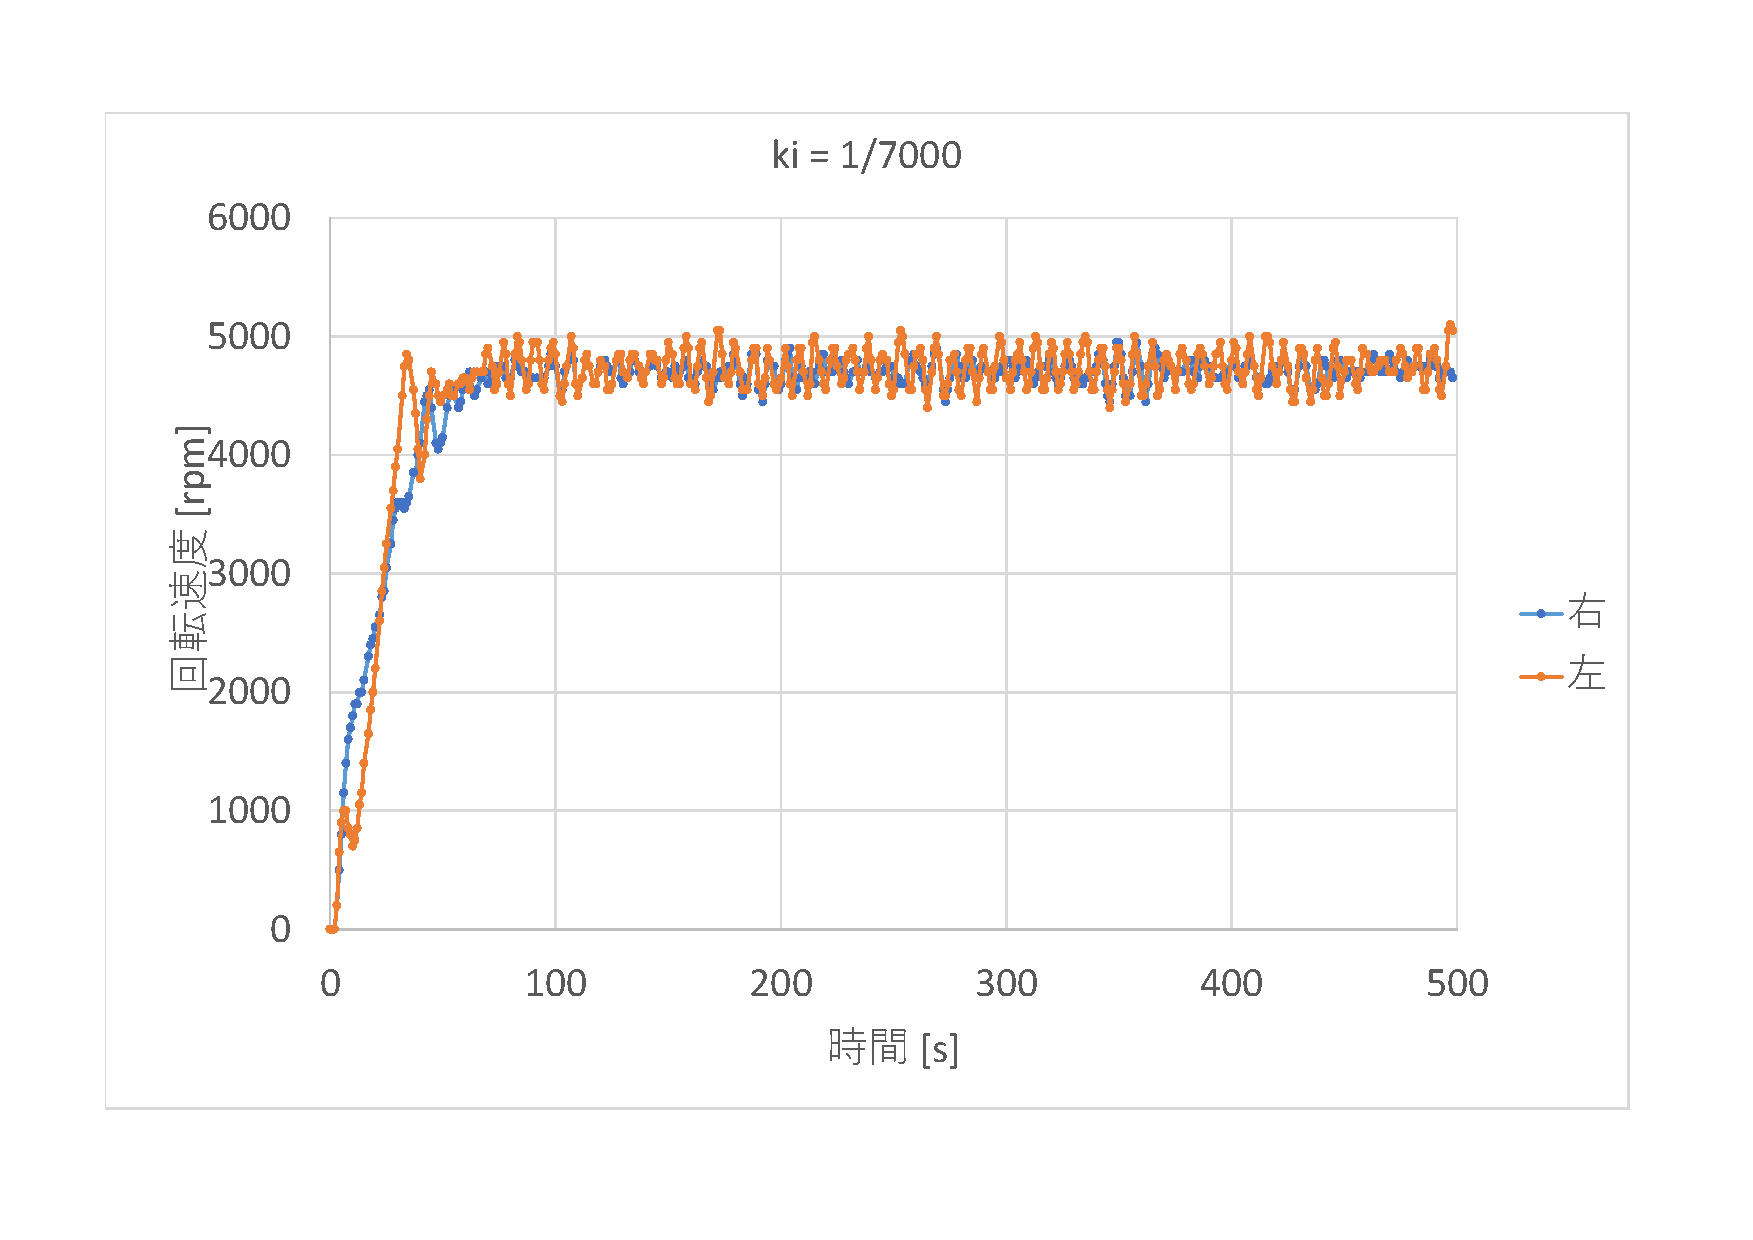
\includegraphics[width=\columnwidth]{img/14/DATA7.pdf}
  \label{im7_14}
  }
  \subfigure[$k_i=1/6000$]{
  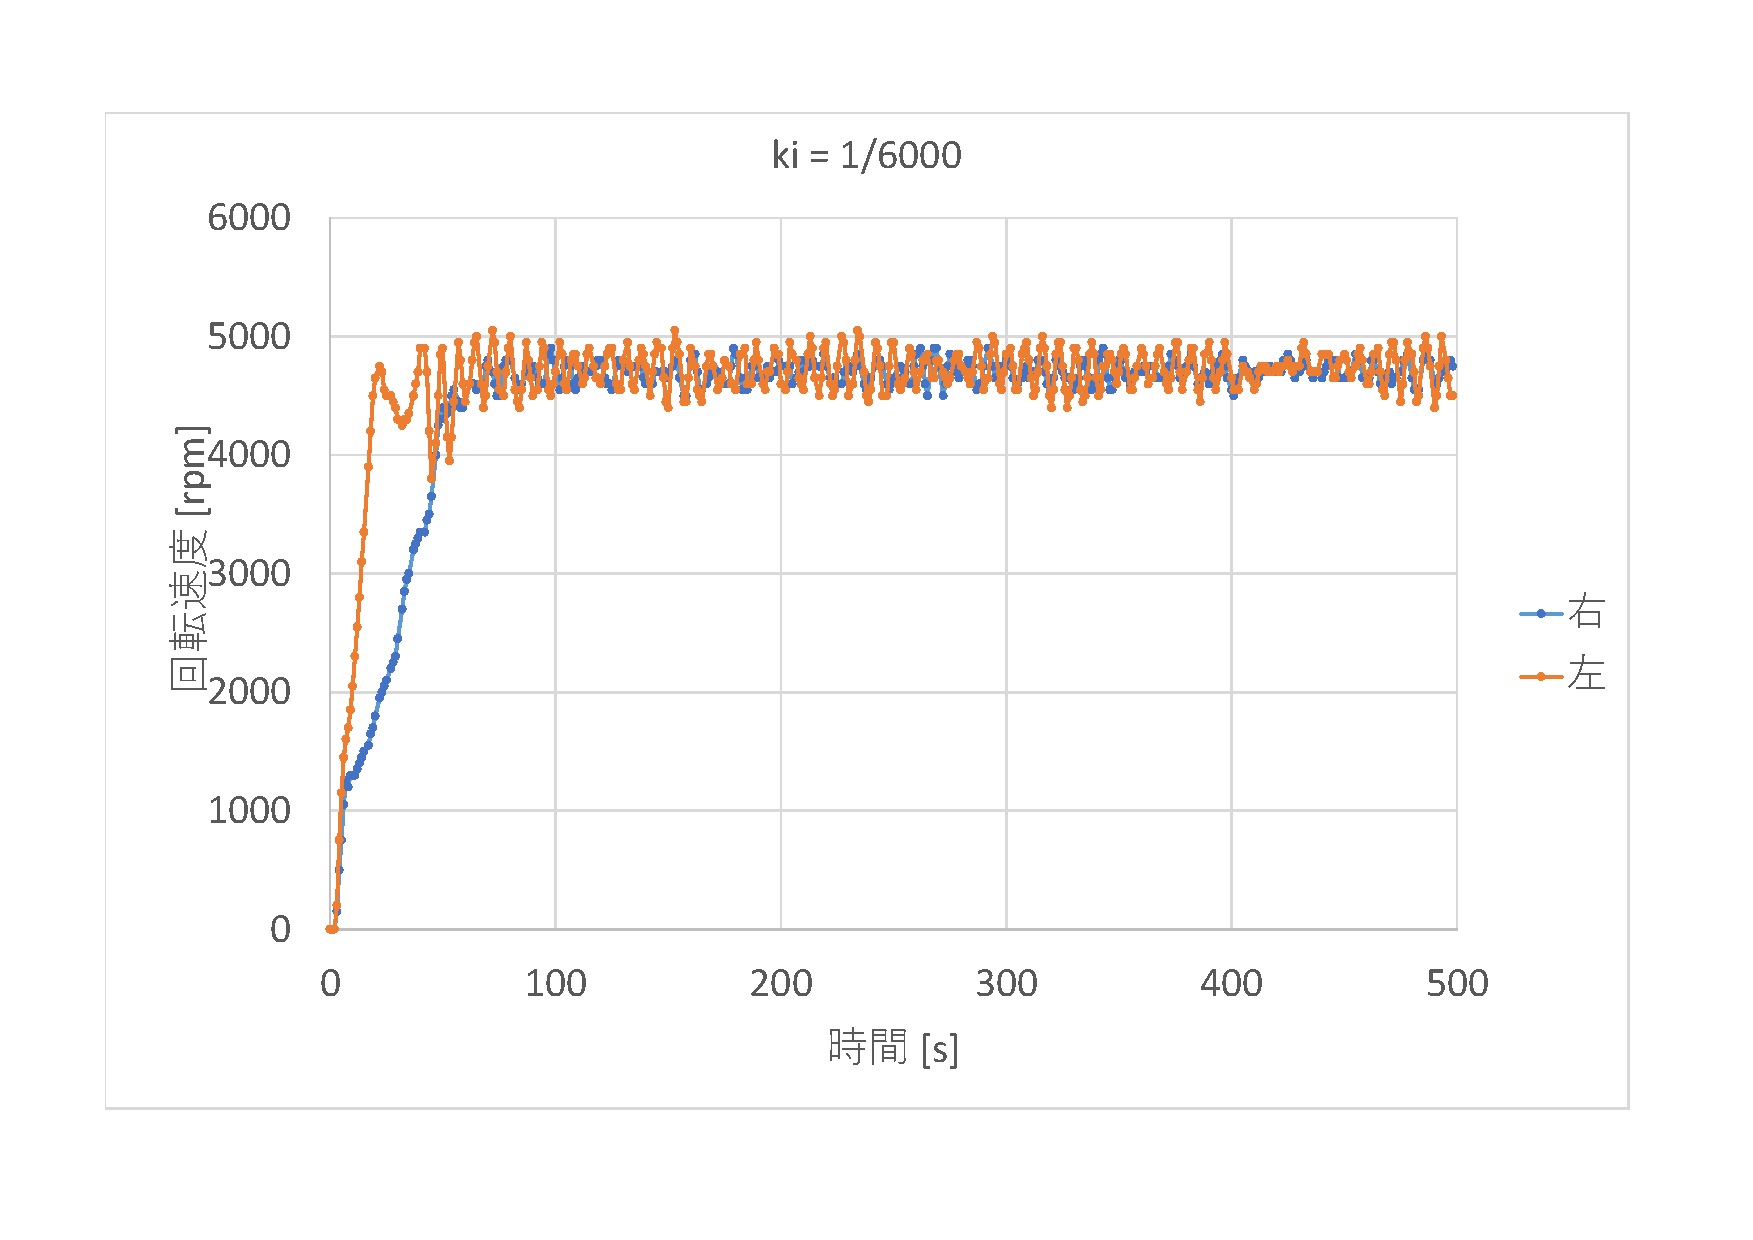
\includegraphics[width=\columnwidth]{img/14/DATA6.pdf}
  \label{im6_14}
  }
  \end{center}
\end{figure}
\begin{figure}[H]
  \begin{center}
  \subfigure[$k_i=1/5000$]{
  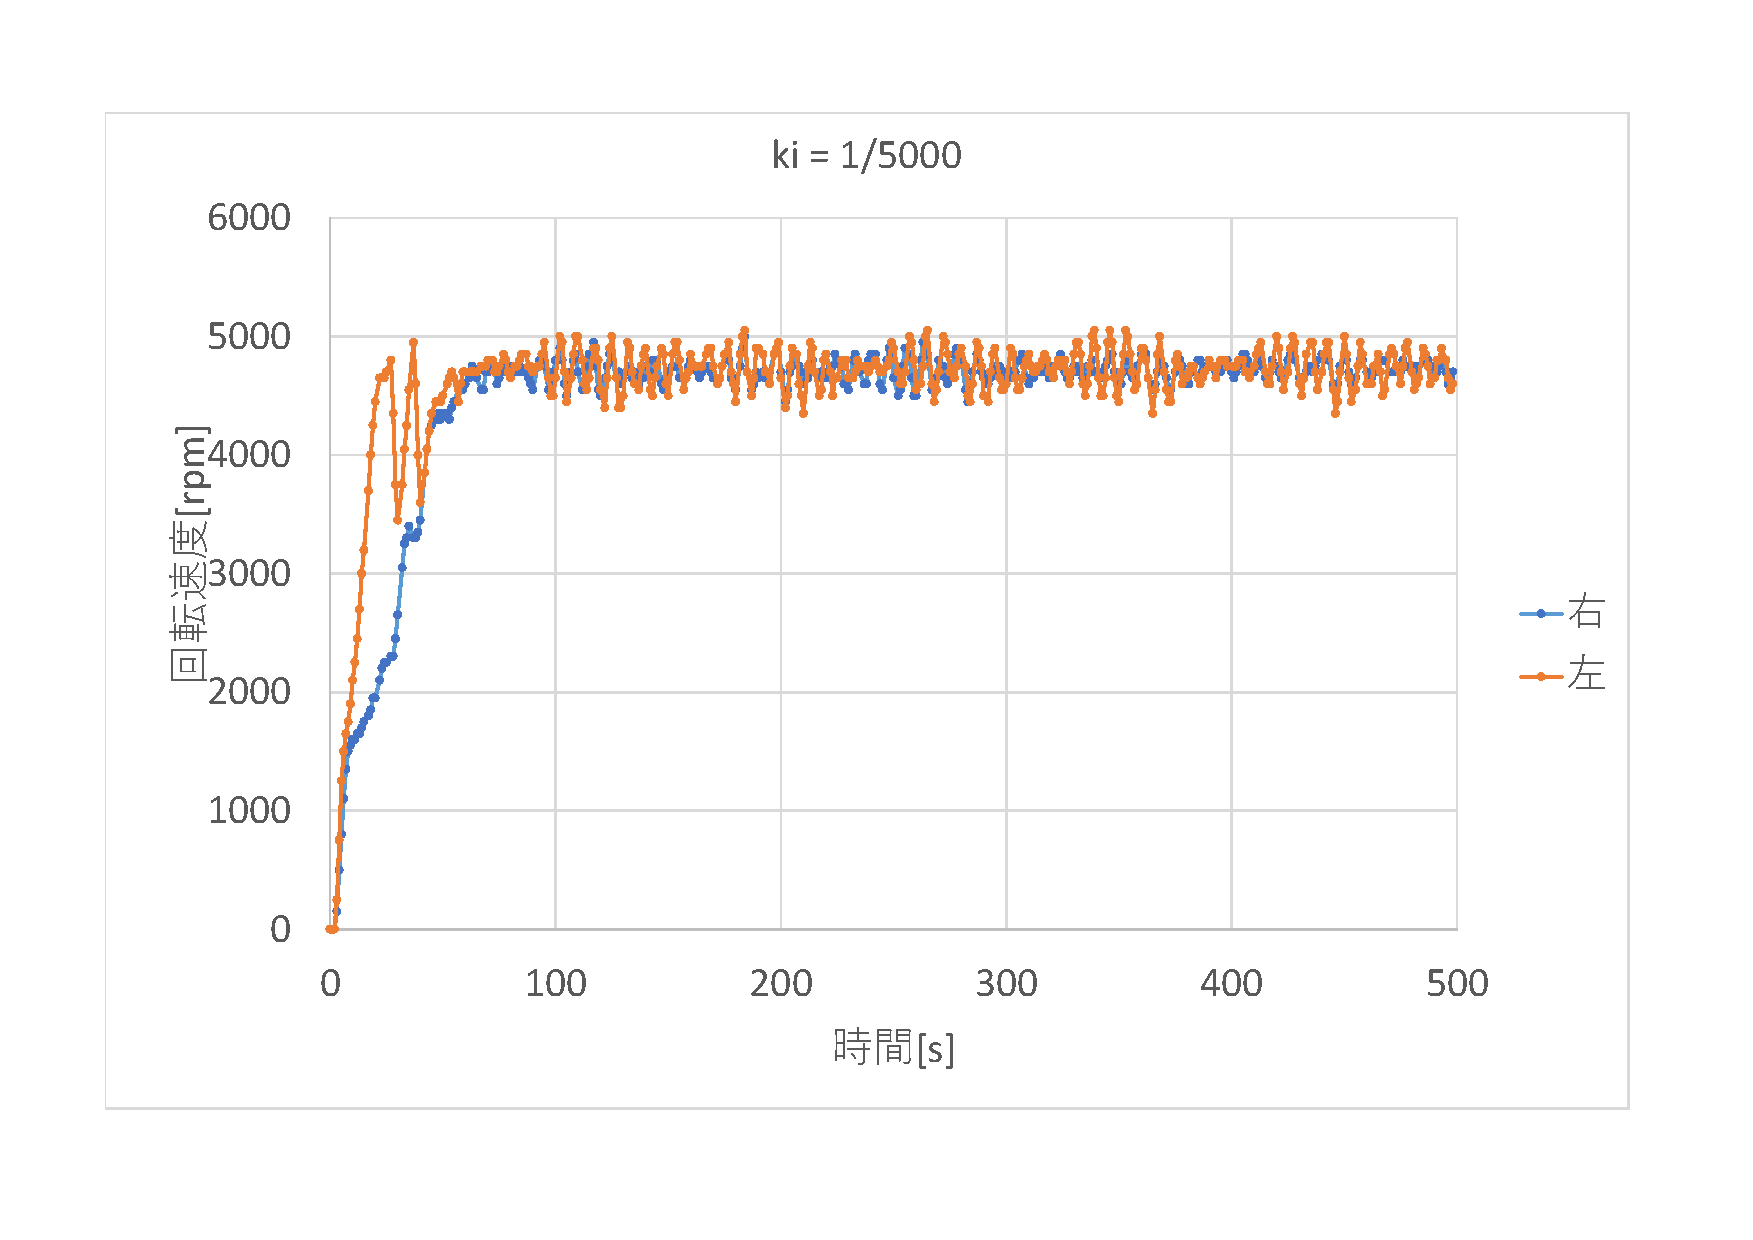
\includegraphics[width=\columnwidth]{img/14/DATA5.pdf}
  \label{im5_14}
  }
  \subfigure[$k_i=1/4000$]{
  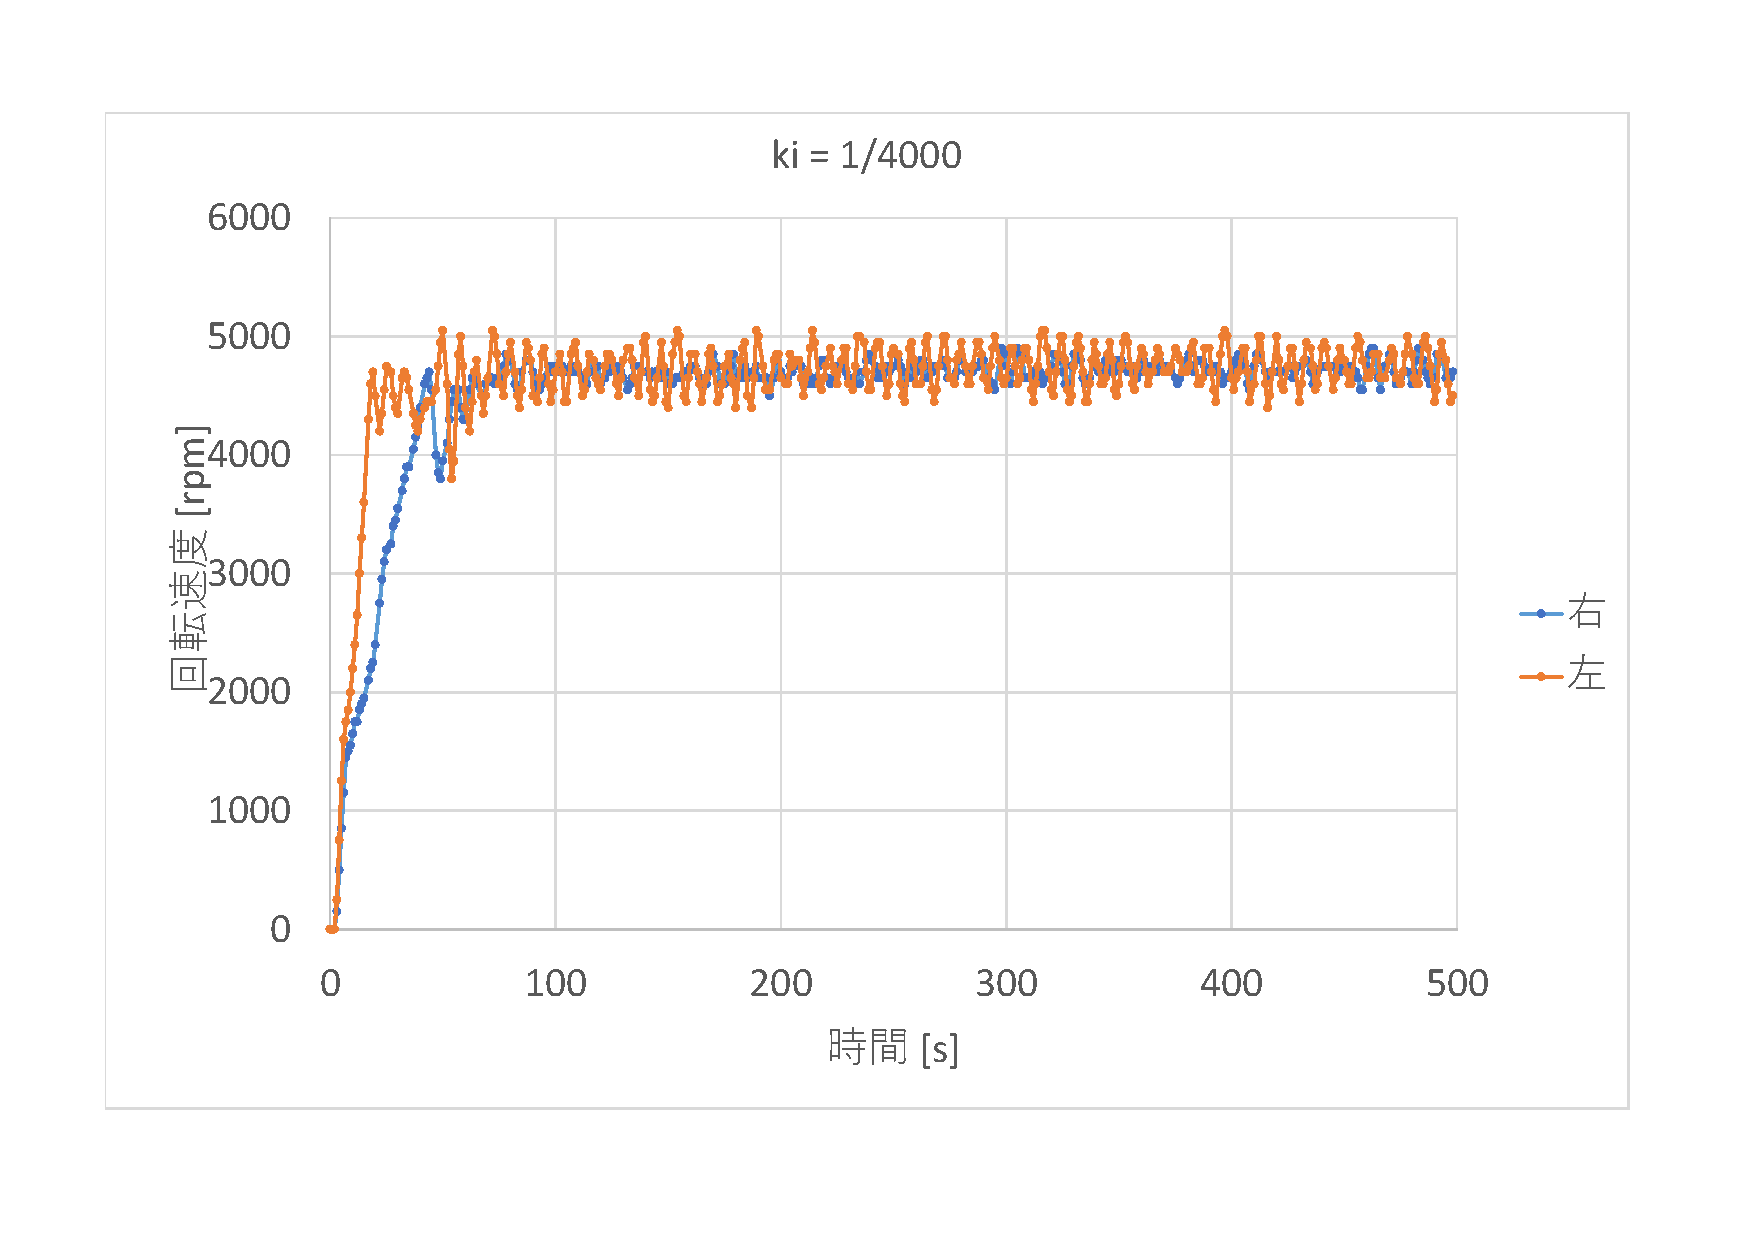
\includegraphics[width=\columnwidth]{img/14/DATA4.pdf}
  \label{im4_14}
  }
  \end{center}
\end{figure}
\begin{figure}[H]
  \begin{center}
  \subfigure[$k_i=1/3000$]{
  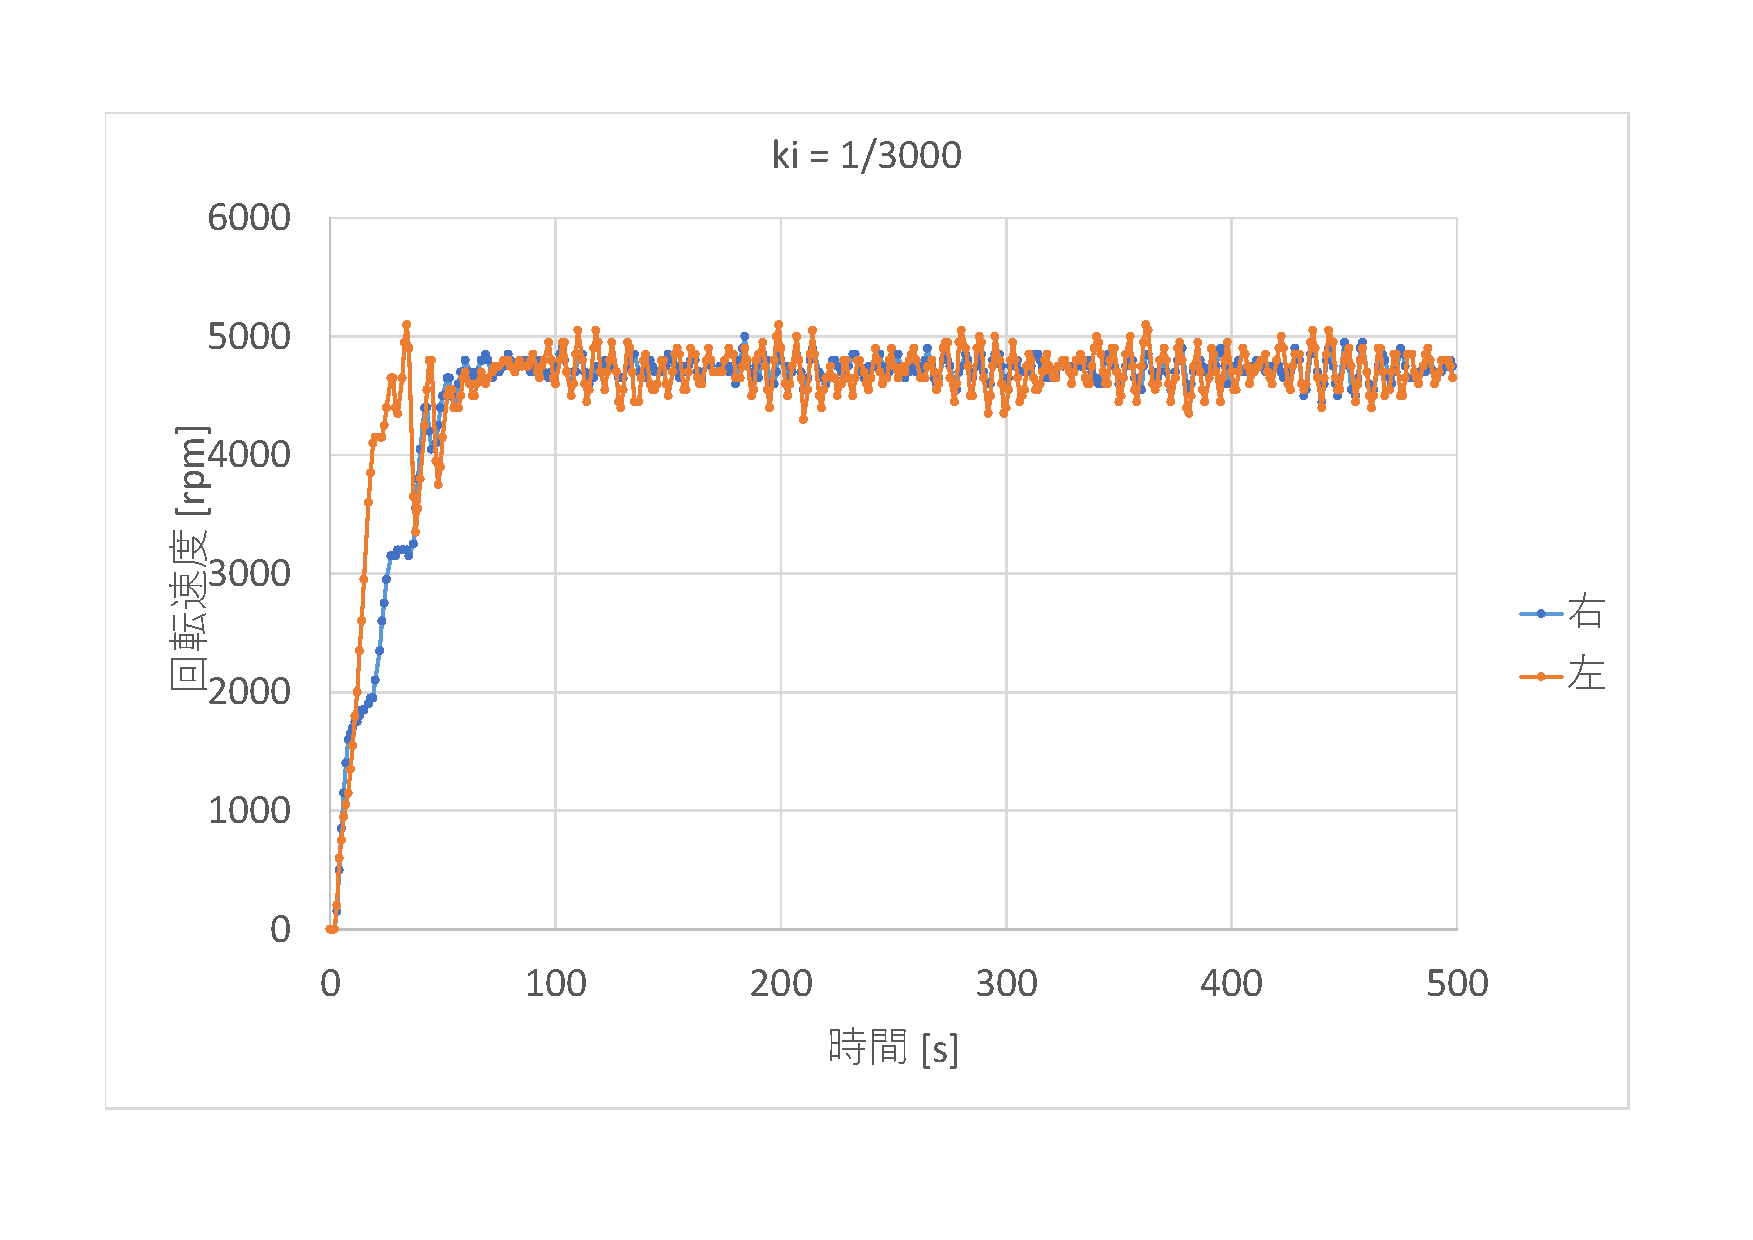
\includegraphics[width=\columnwidth]{img/14/DATA3.pdf}
  \label{im3_14}
  }
  \subfigure[$k_i=1/2000$]{
  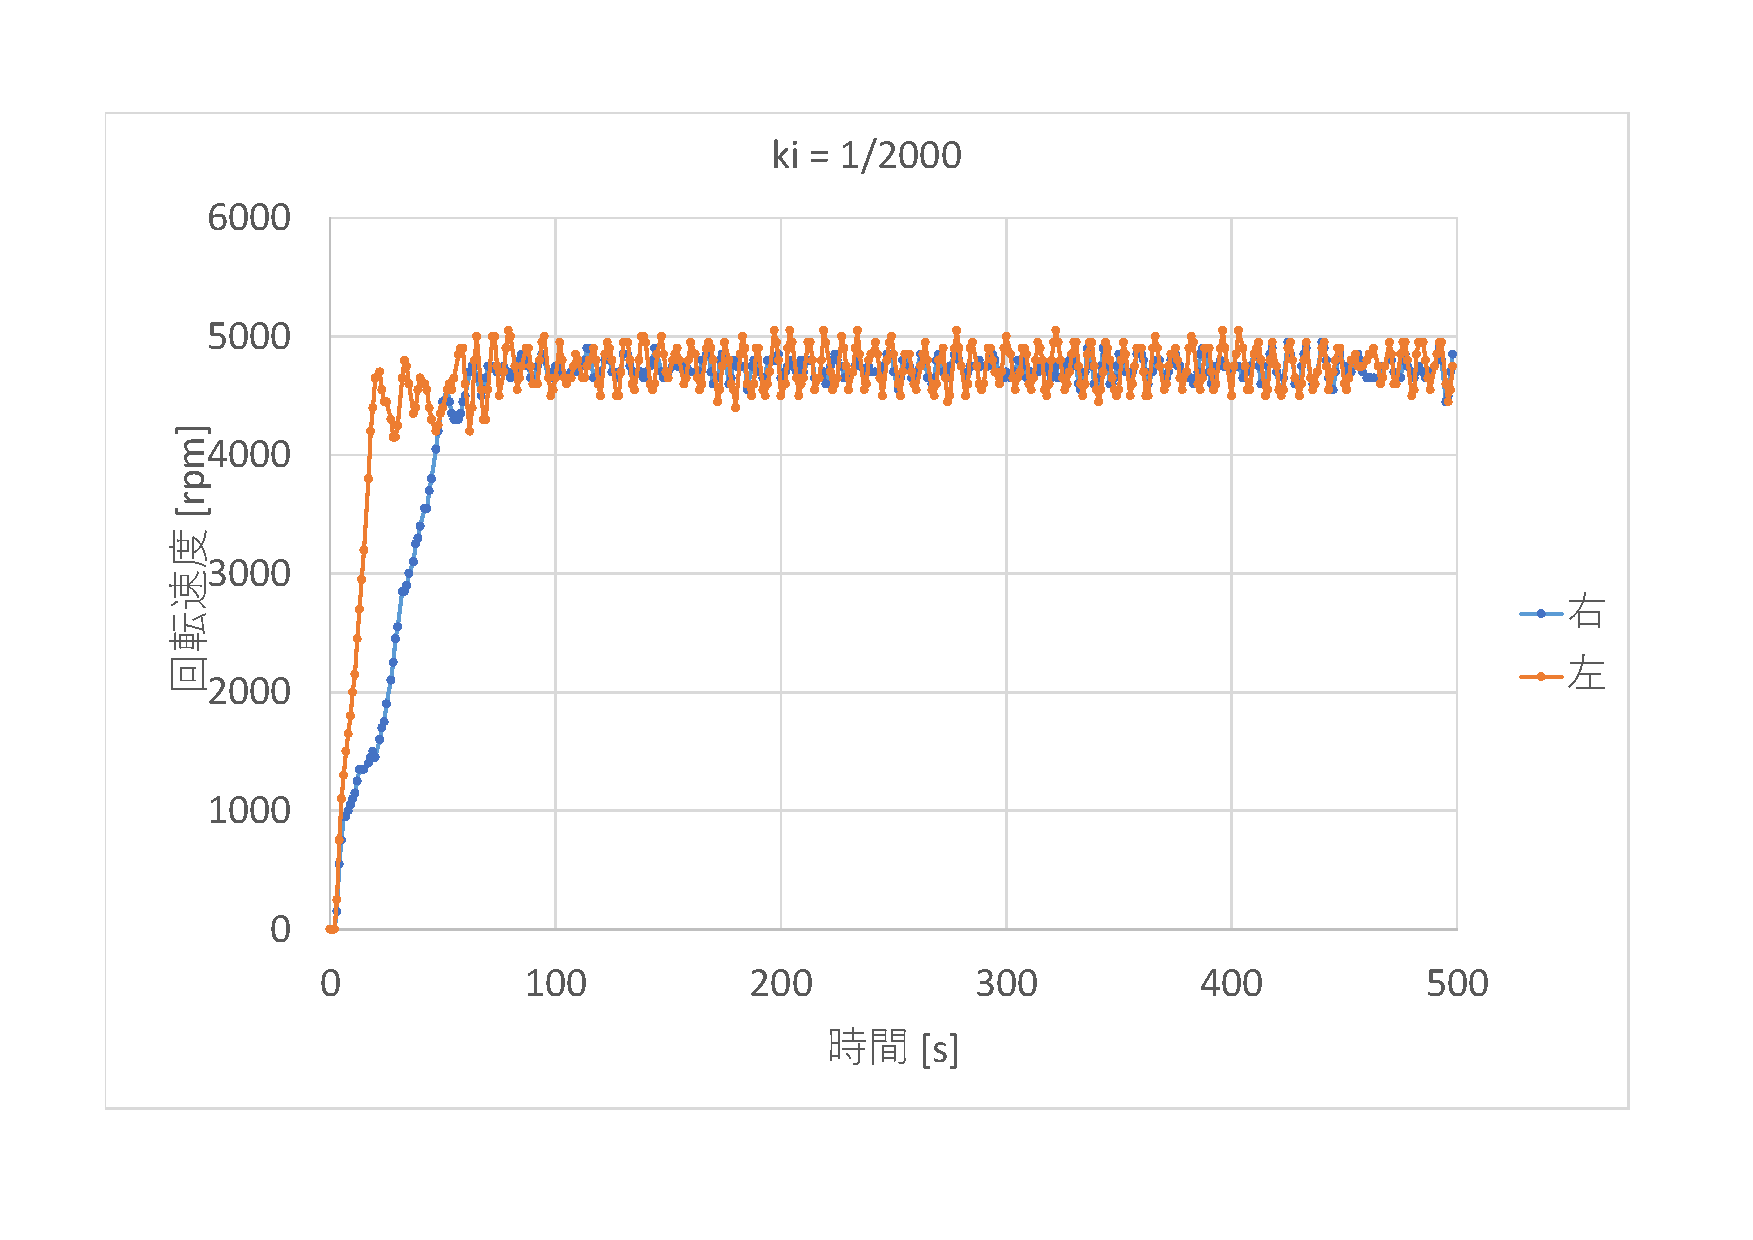
\includegraphics[width=\columnwidth]{img/14/DATA2.pdf}
  \label{im2_14}
  }
  \end{center}
\end{figure}
\begin{figure}[H]
  \begin{center}
  \subfigure[$k_i=1/1000$]{
  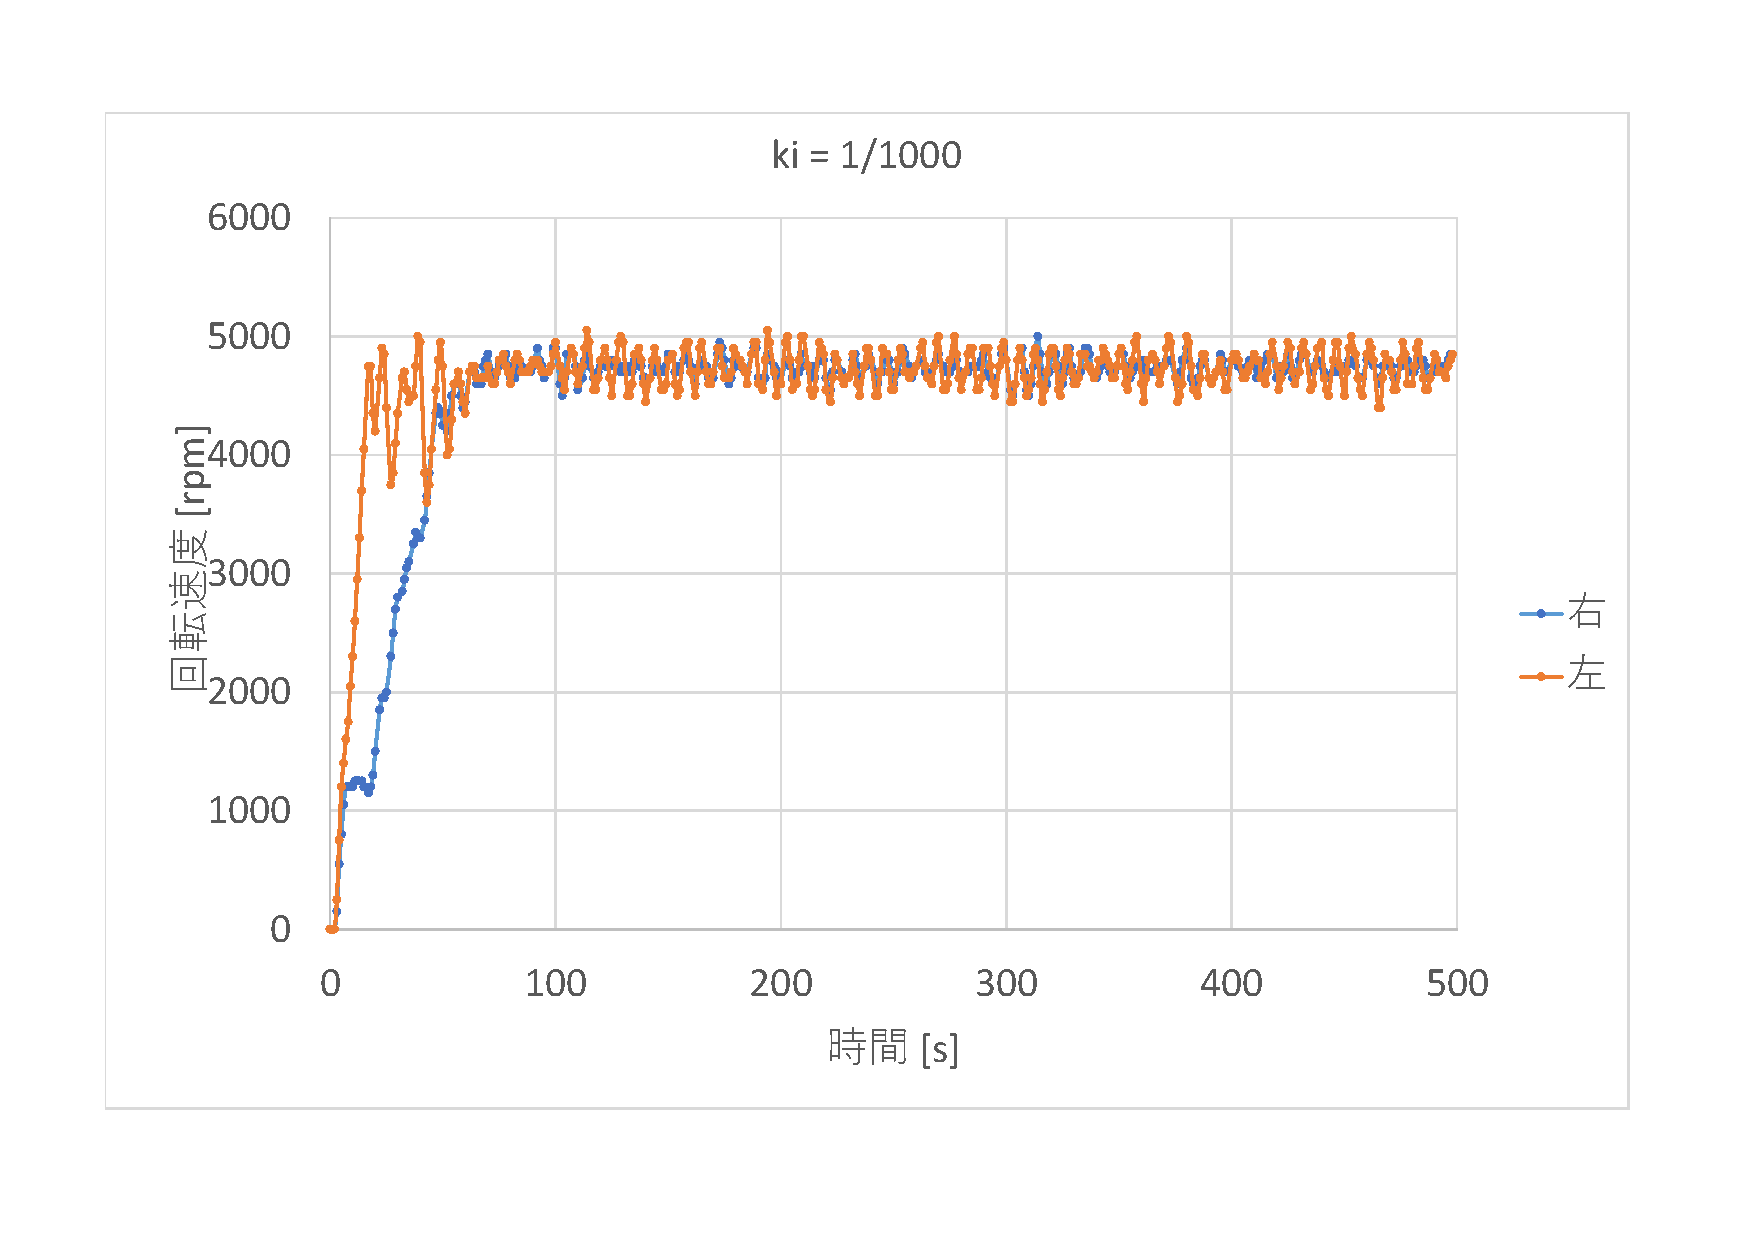
\includegraphics[width=\columnwidth]{img/14/DATA1.pdf}
  \label{im1_14}
  }
  \caption{ステップ応答のグラフ}
  \end{center}
\end{figure}
\section{演習15}
\subsection{実行プログラム}
実行プログラムをソースコード\ref{s15}に示す。

\begin{lstlisting}[caption=演習15のプログラム,label=s15]
#include <stdio.h>
#include <process.h> /*exit関数の定義*/
#include <dos.h>
#include "v25.h"
#include "ms.h"
  
#define DMAX 10000
#define INTERVAL 100
#define DISTANCE 3000
  
int main(){
    int i, n=0;
    int kp = 3, ki_inv = 10000;
  
    int vref[11] = {1000, 2000, 3000, 4000, 5000, 6000,
                    5000, 4000, 3000, 2000, 1000};
    long time[11] = {200, 200, 200, 200, 200, 1040,
                    200, 200, 200, 200, 200};
    long j=0, cl, cl0, cr, cr0, ct, ct0, ctm, l[DMAX], r[DMAX], t[DMAX];
    FILE *fp;
  
    ms_init();
    ms_motor_on();
    ms_set_gain(kp, ki_inv);
    ms_read_c(&cl0, &cr0, &ct0);
    ctm = ct0;
    for(i=0; i<11; i++){
        ms_set_v(vref[i], vref[i]);
        do{
            ms_read_c(&cl, &cr, &ct);
            n = j/INTERVAL;
            l[n] = cl;
            r[n] = cr;
            t[n] = ct;
            j++;
        }while(time[i]>ct-ctm);
        ctm = ct;
    }
    ms_motor_off();
 
    if((fp = fopen("data.dat", "wt")) == NULL){
        printf("Can't Open File!!\n");
        exit(1);
    }

    for(i=0; i<=n; i++){
        fprintf(fp, "%12.6lf %12.6lf %5ld\n",
        DISTANCE-15*2*3.14159*(l[i]-cl0)/(19.225*400),
        DISTANCE-15*2*3.14159*(r[i]-cr0)/(19.225*400),
        t[i]-ct0);
    }
    fclose(fp);
    ms_beep(440,500);
    return 0;
}
\end{lstlisting}

\subsection{実行結果}
演習14と同様に
モータの応答(回転速度と目標位置までの距離)を
負荷無し、有りの場合分けをしてデータファイルに保存する。
負荷無し、有りの場合を図\ref{fuka_15}、\ref{non_15}に示す。
負荷有りの場合、ロボットは前進しない。
負荷無しの場合、ロボットは目標位置に近づくことが分かる。

\begin{figure}
  \begin{center}
    \subfigure[負荷有り]{
    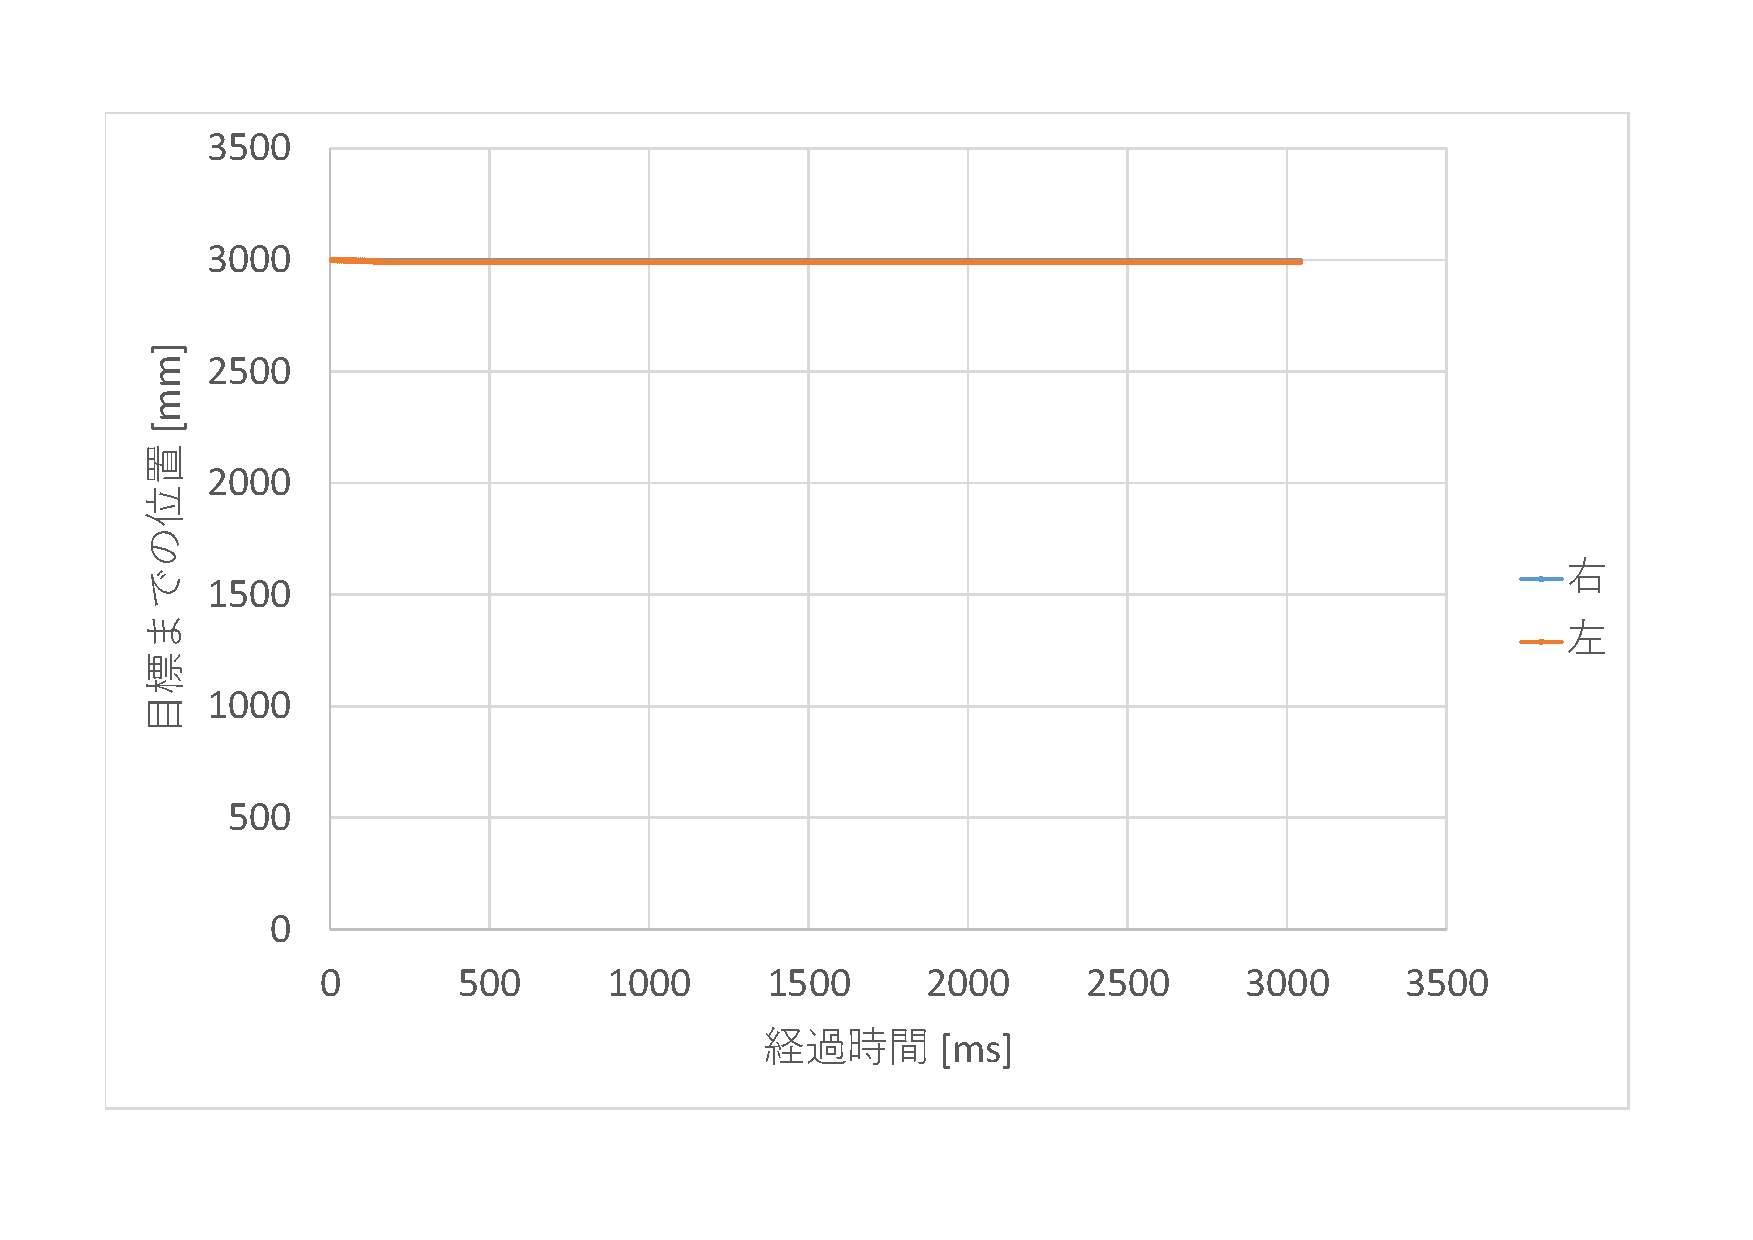
\includegraphics[width=\linewidth]{img/15/15_fuka.pdf}
    \label{fuka_15}
    }
    \subfigure[負荷無し]{
    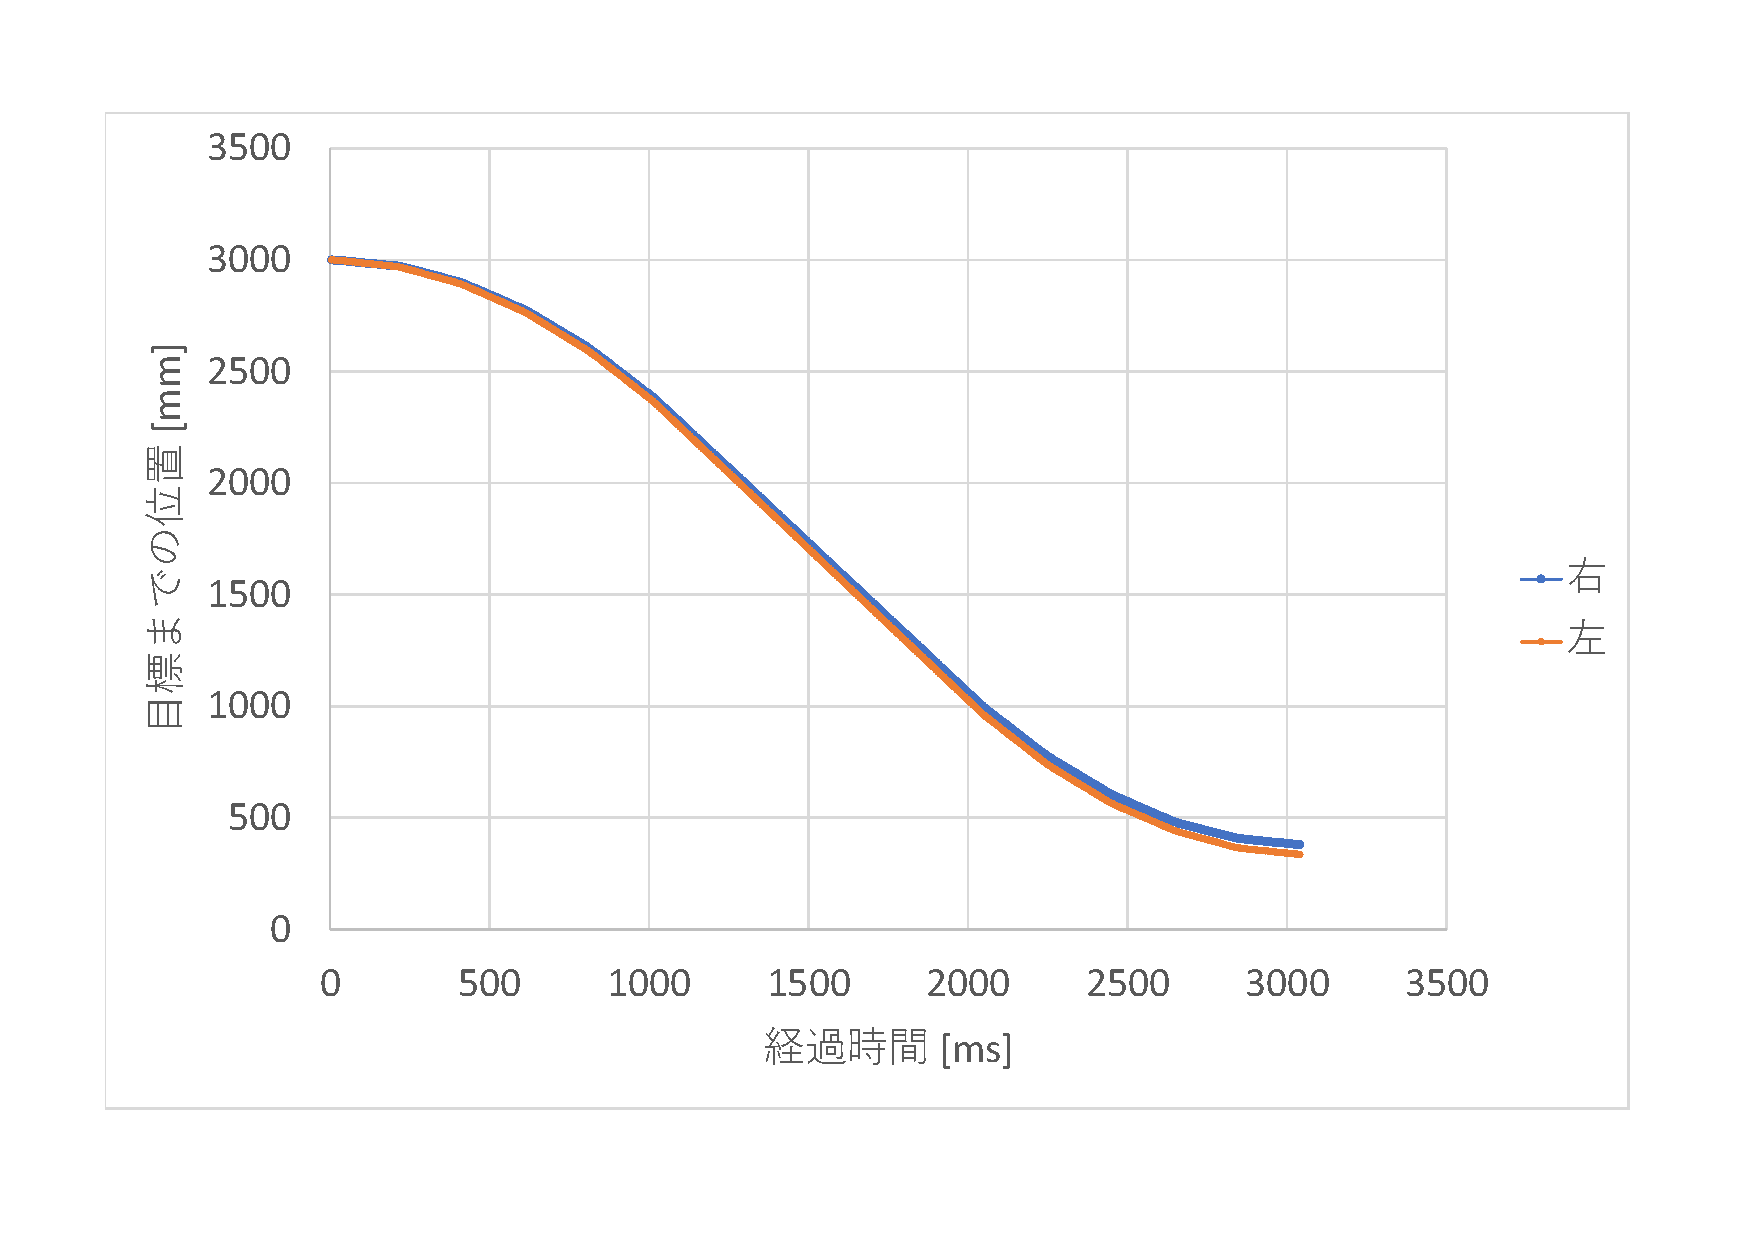
\includegraphics[width=\linewidth]{img/15/15_non.pdf}
    \label{non_15}
    }
  \caption{モータの応答}
  \end{center}
\end{figure}


\section{演習16}
\subsection{実行プログラム}
実行プログラムをソースコード\ref{s16}に示す。
\begin{lstlisting}[caption=演習16のプログラム,label=s16]
#include <stdio.h>
#include <process.h>    /*exit関数の定義*/
#include <dos.h>        /*pokeb関数の定義*/
#include "v25.h"        /*V25固有値の定義*/
#include "ms.h"         /*ms関数の定義*/
   
#define DMAX 10000      /*保存データ数の最大値*/
#define INTERVAL 100    /*保存データの間隔*/
#define INTERVAL2 5     /*保存データの間隔*/
#define DISTANCE 3000   /*ロボットの移動距離*/
#define C_DISTANCE ((DISTANCE*400.*19.225)/(15.*2.*3.14159))
                          /*ロボットの移動距離(カウンタ換算)*/
#define THRESH 100      /*閾値*/
   
int main()
{
    int i, n = 0, n2 = 0, k = 5;
    int kp = 6, ki_inv = 10000;     /*FBゲイン*/
    /*速度パターン*/
    int vref[6] = {1000, 2000, 3000, 4000, 5000, 6000};
    long time[5] = {200, 200, 200, 200, 200};
    long j = 0, cl, cl0, cr, cr0, ct, ct0, ctm, el, er, vl, vr, l[DMAX], r[DMAX], t[DMAX];
    FILE *fp;
  
    ms_init();                          /*初期化*/
    ms_motor_on();                      /*モータ回路ON*/
    ms_set_gain( kp, ki_inv );          /*FBゲインの設定*/
    ms_read_c( &cl0, &cr0, &ct0 );      /*カウンタ値の初期値の取得*/
    ctm=ct0;
    for( i = 0; i < 5; i++)
    {
        ms_set_v( vref[i], vref[i] );   /*速度の設定*/
        do
        {
            ms_read_c( &cl, &cr, &ct ); /*カウンタ値の読み込み*/
            n = j/INTERVAL;
            l[n] = cl;
            r[n] = cr;
            t[n] = ct;
            j++;
        } while ( time[i] > ct-ctm );   /*時間間隔のチェック*/
        ctm = ct;
    }
    j = 0;
    do
    {
        el = C_DISTANCE - cl;           /*目標値との偏差を算出*/
        er = C_DISTANCE - cr;           
        vl = k * el;                    /*速度の計算*/
        vr = k * er;
        if ( vl > vref[5] )             /*最高速度の設定*/
        {
          vl = vref[5];
        }
        if ( vr > vref[5] )
        {
          vr = vref[5];
        }
        ms_set_v( vl, vr );             /*速度の設定*/
        ms_read_c( &cl, &cr, &ct );     /*カウンタ値の読み込み*/
        n2 = j/INTERVAL2 + n + 1;
        l[n2] = cl;
        r[n2] = cr;
        t[n2] = ct;
        j++; 
    } while ( n2<DMAX && el>THRESH && er>THRESH );  /*終了条件のチェック*/
        
    ms_motor_off();                     /*モータ回路OFF*/
    /*保存ファイルのオープン*/
    if ((fp = fopen("data.dat","wt")) == NULL)
    {
      printf("Can't open file.\n");
      exit(1);
    }
    /*ファイルの保存*/
    for ( i = 0; i < n2; i++)
    {
      fprintf(fp,"%12.6lf %12.6lf %5ld\n",DISTANCE-15*2*3.14159*(l[i]-cl0)/(19.225*400),DISTANCE-15*2*3.14159*(r[i]-cr0)/(19.225*400),t[i]-ct0);
    }
    fclose(fp);                     /*ファイルのクローズ*/
    return 0;
}
\end{lstlisting}

\subsection{実行結果}
負荷有りの場合、目標位置までの距離の変化率が左右のモータで均等でない。
ロボットの重心が、左右で均等でなかったためであると考えられる。
負荷無しの場合、目標位置までの距離が単調的に減少し、目標位置に近づくことが分かる。
\begin{figure}[H]
  \begin{center}
    \subfigure[負荷有り]{
    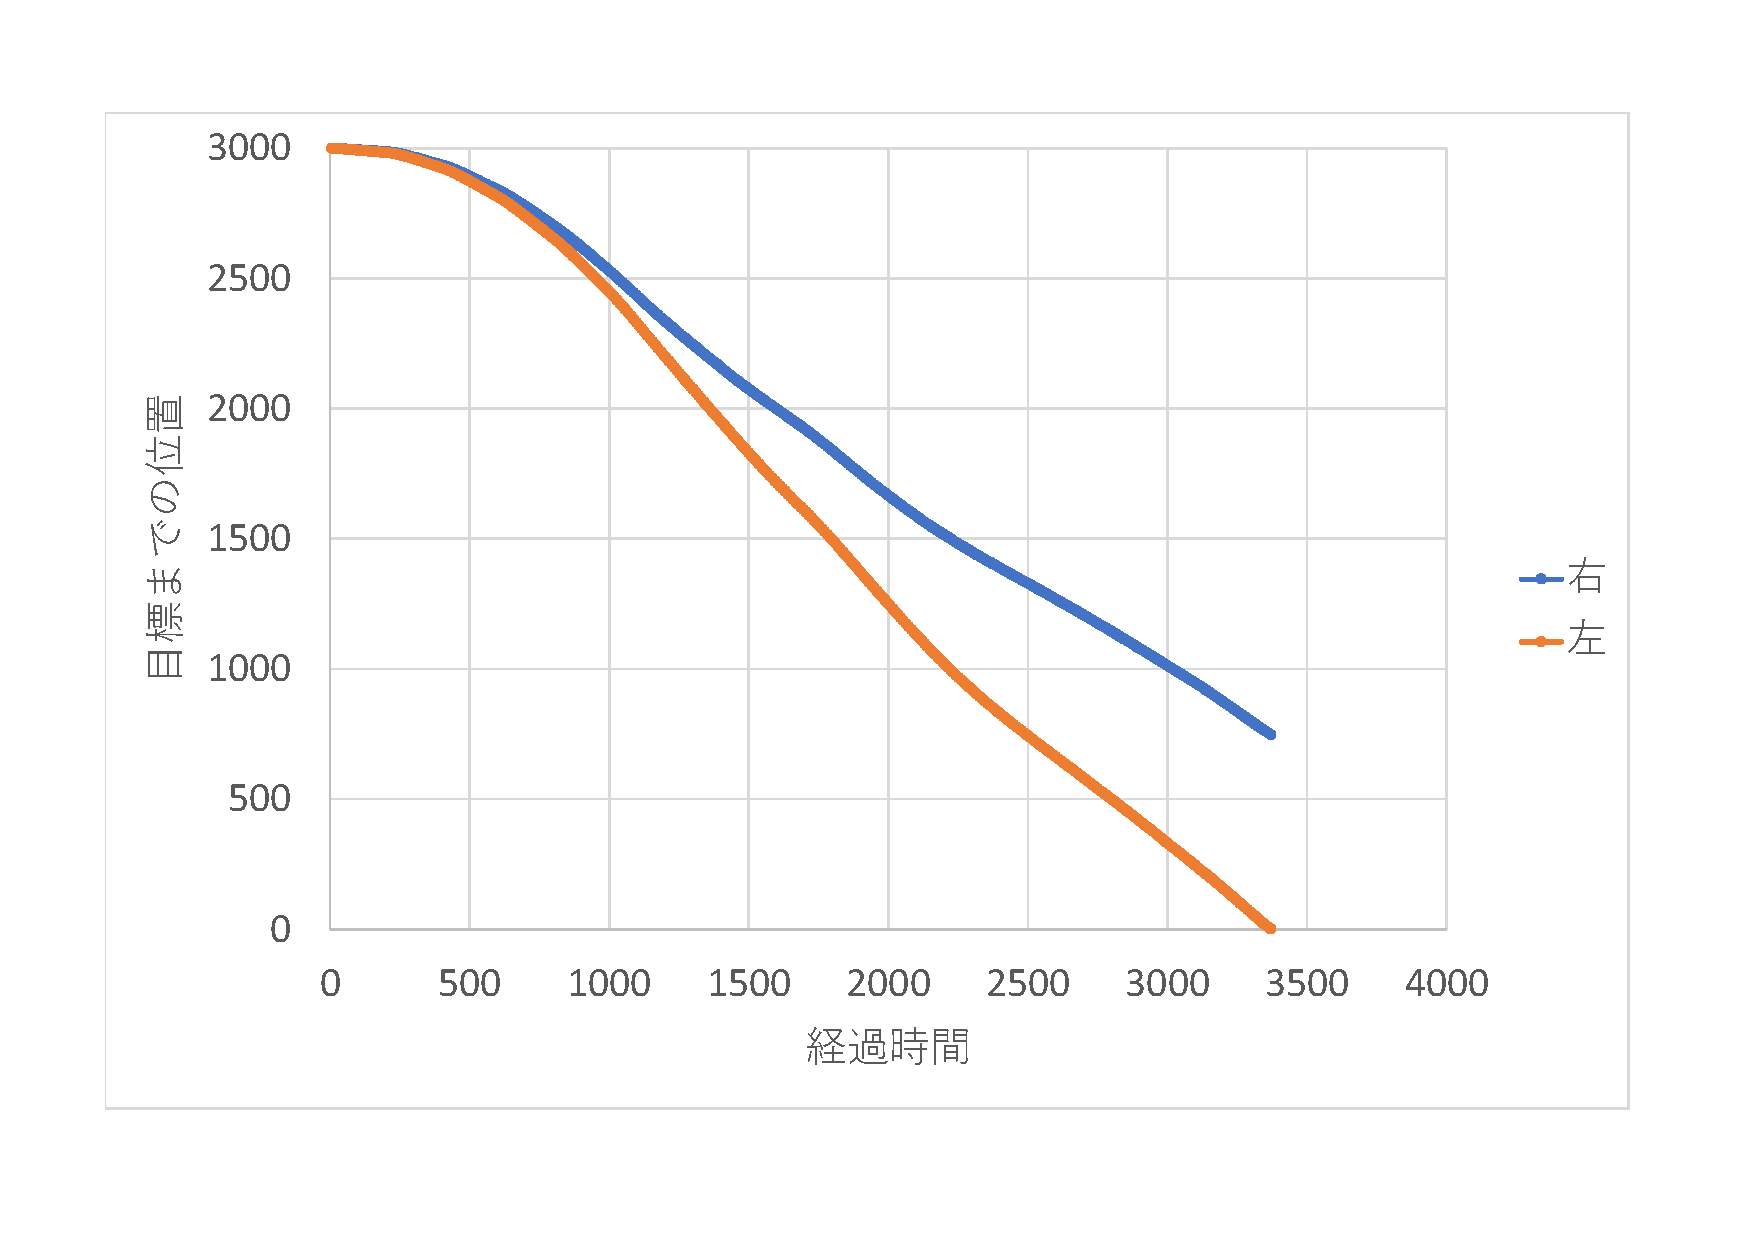
\includegraphics[width=\linewidth]{img/16/16_fuka.pdf}
    }
    \subfigure[負荷無し]{
    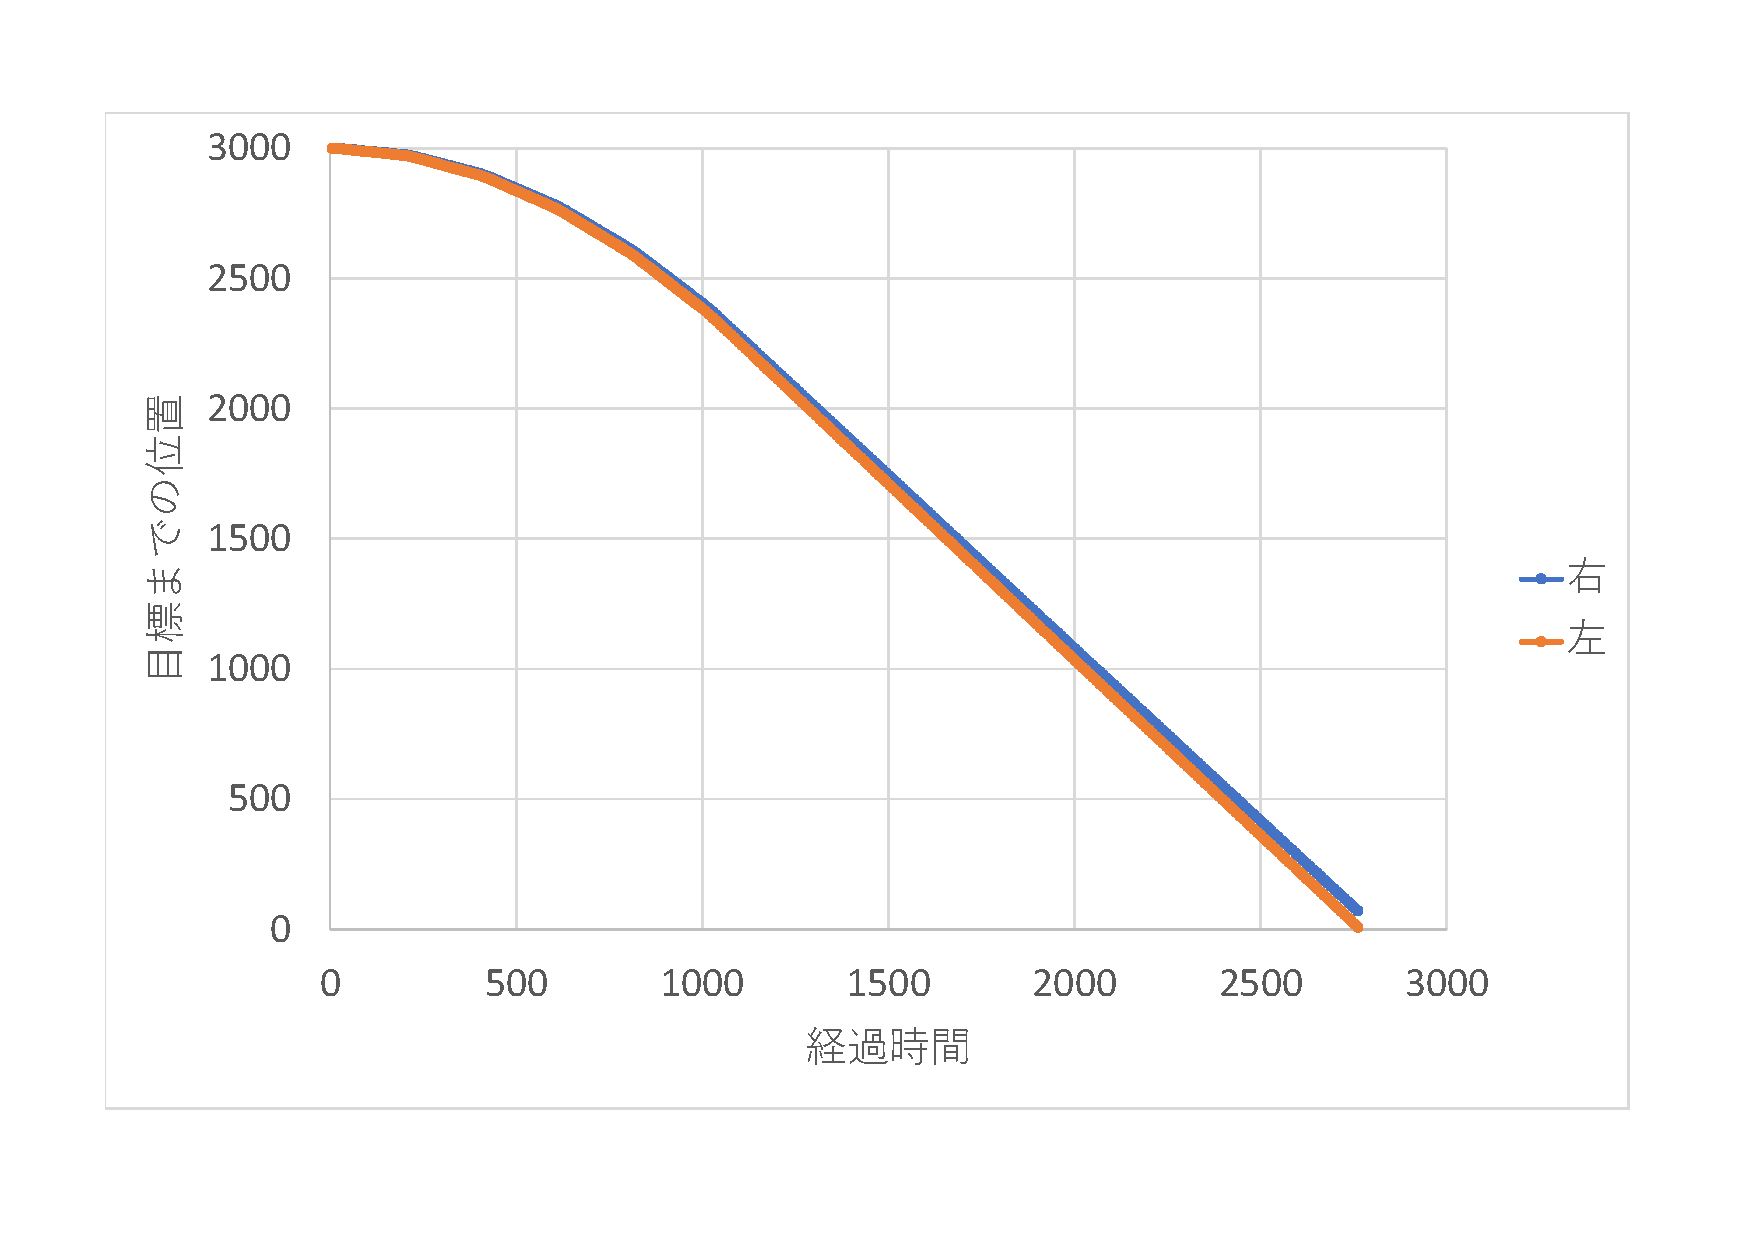
\includegraphics[width=\linewidth]{img/16/16_non.pdf}
    }
  \end{center}
\end{figure}

\section{演習17}
\subsection{実行プログラム}
実行プログラムをソースコード\ref{s17}に示す。
\begin{lstlisting}[caption=演習17のプログラム,label=s17]
#include <stdio.h>
#include <process.h>
#include <dos.h>
#include "v25.h"
#include "ms.h"

#define DMAX 10000
#define INTERVAL 100
#define INTERVAL2 5
#define DISTANCE 3000
#define C_DISTANCE ((DISTANCE*400.*19.225)/(15.*2.*3.14159))
#define THRESH 100
  
int main()
{
    int i, n = 0, n2 = 0;
    double k = ms_read_dip();
    int kp = 3, ki_inv = 10000;
  
    int vref[6] = {1000, 2000, 3000, 4000, 5000, 6000};
    long time[5] = {200, 200, 200, 200, 200};
    long j = 0, cl, cl0, cr, cr0, ct, ct0, ctm, el, er, vl, vr, l[DMAX], r[DMAX], t[DMAX];
    FILE *fp;
  
    ms_init();
    ms_motor_on();
    ms_set_gain( kp, ki_inv );
    ms_read_c( &cl0, &cr0, &ct0 );
    ctm=ct0;
    for( i = 0; i < 5; i++)
    {
        ms_set_v( vref[i], vref[i] );
        do
        {
            ms_read_c( &cl, &cr, &ct );
            n = j/INTERVAL;
            l[n] = cl;
            r[n] = cr;
            t[n] = ct;
            j++;
        } while ( time[i] > ct-ctm );
        ctm = ct;
    }
    j = 0;
    do
    {
        el = C_DISTANCE - cl;
        er = C_DISTANCE - cr;
        vl = k * el;
        vr = k * er;
        if ( vl > vref[5] )
        {
            vl = vref[5];
        }
        if ( vr > vref[5] )
        {
            vr = vref[5];
        }
        ms_set_v( vl, vr );
        ms_read_c( &cl, &cr, &ct );
        n2 = j/INTERVAL2 + n + 1;
        l[n2] = cl;
        r[n2] = cr;
        t[n2] = ct;
        j++; 
    } while ( n2<DMAX && el>THRESH && er>THRESH );
      
    ms_motor_off();
  
    if ((fp = fopen("data.dat","wt")) == NULL)
    {
        printf("Can't open file.\n");
        exit(1);
    }

    for ( i = 0; i < n2; i++)
    {
        fprintf(fp,"%12.6lf %12.6lf %5ld\n",DISTANCE-15*2*3.14159*(l[i]-cl0)/(19.225*400),DISTANCE-15*2*3.14159*(r[i]-cr0)/(19.225*400),t[i]-ct0);
    }
    fclose(fp);
  
    printf("owari\n");
    ms_beep(440,500);
    return 0;
}
\end{lstlisting}
\mysubsection{実行結果}
実行結果を図\ref{im32}から\ref{im41}に示す。
$k = 1$において、ロボットが目標位置に到着した際に転倒し、
距離データの記録が5000秒付近まで続いている。

また、負荷有りよりも負荷無しの方が、目標位置への所要時間が少ない。
位置のフィードバックゲインの値を大きくすると、目標位置までの所要時間が減少する。


\begin{figure}
  \begin{center}
  \subfigure[$k=1$ 負荷有り]{
  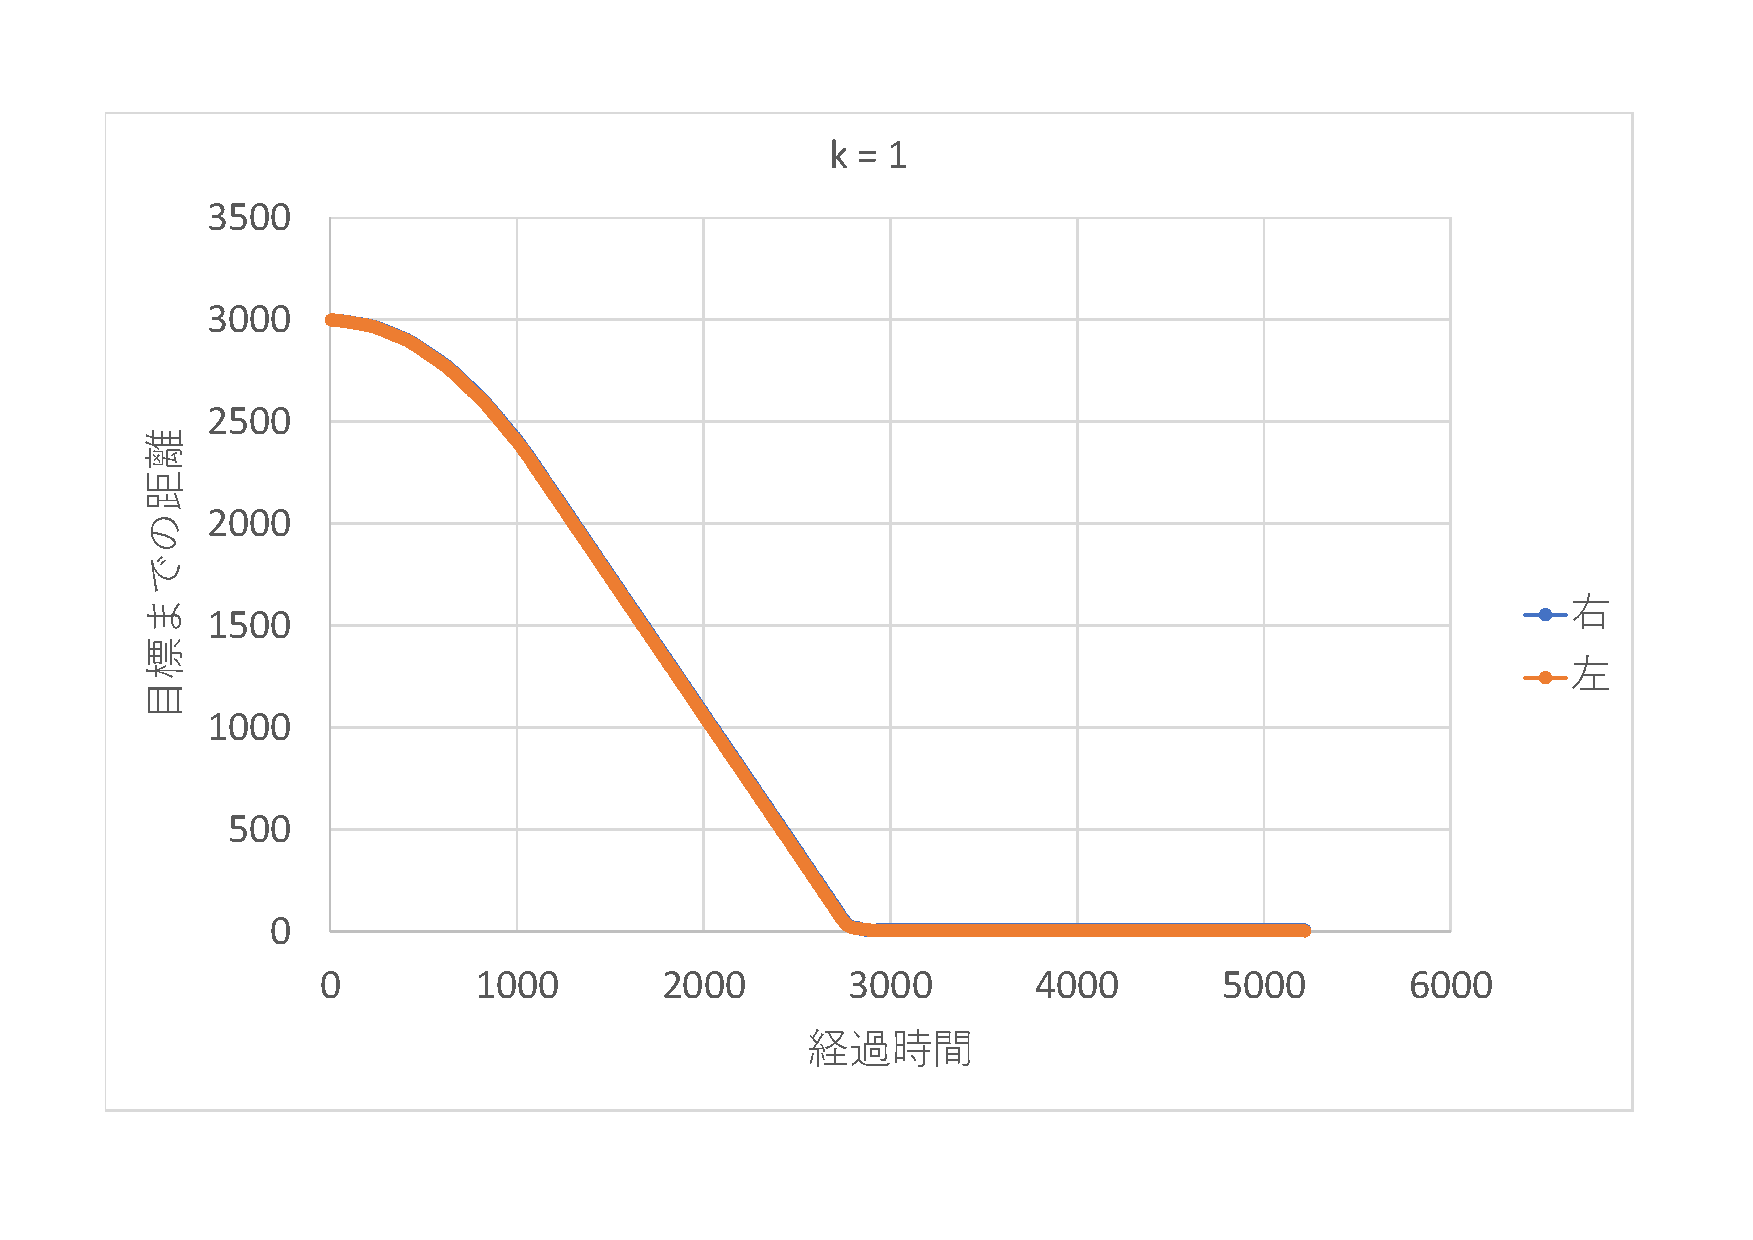
\includegraphics[width=\linewidth]{img/17/17_fuka_K1.pdf}
  \label{im32}
  }
  \subfigure[$k=1$ 負荷無し]{
  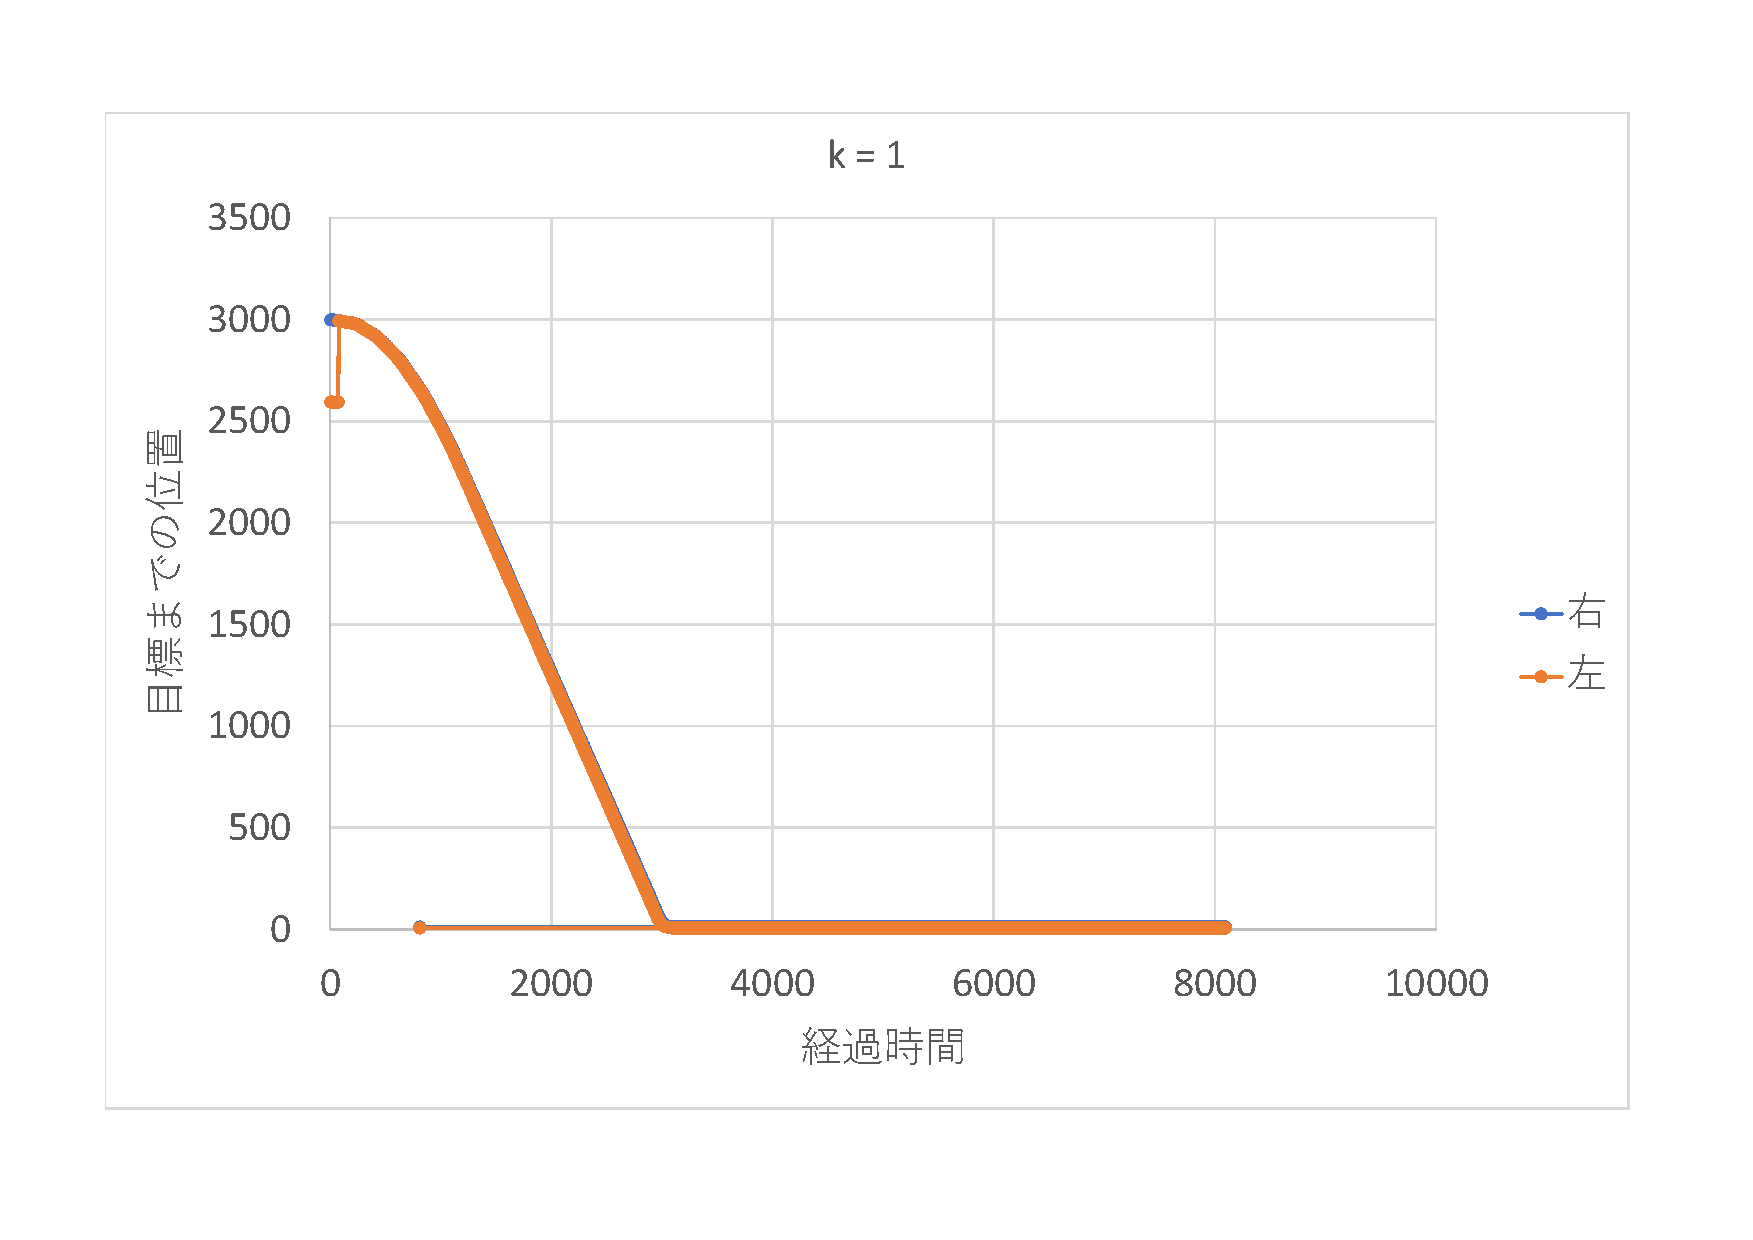
\includegraphics[width=\linewidth]{img/17/17_non_K1.pdf}
  \label{im33}
  }
  \caption{$k = 1$のステップ応答}
  \end{center}
\end{figure}

\begin{figure}
  \begin{center}
  \subfigure[$k=2$ 負荷有り]{
  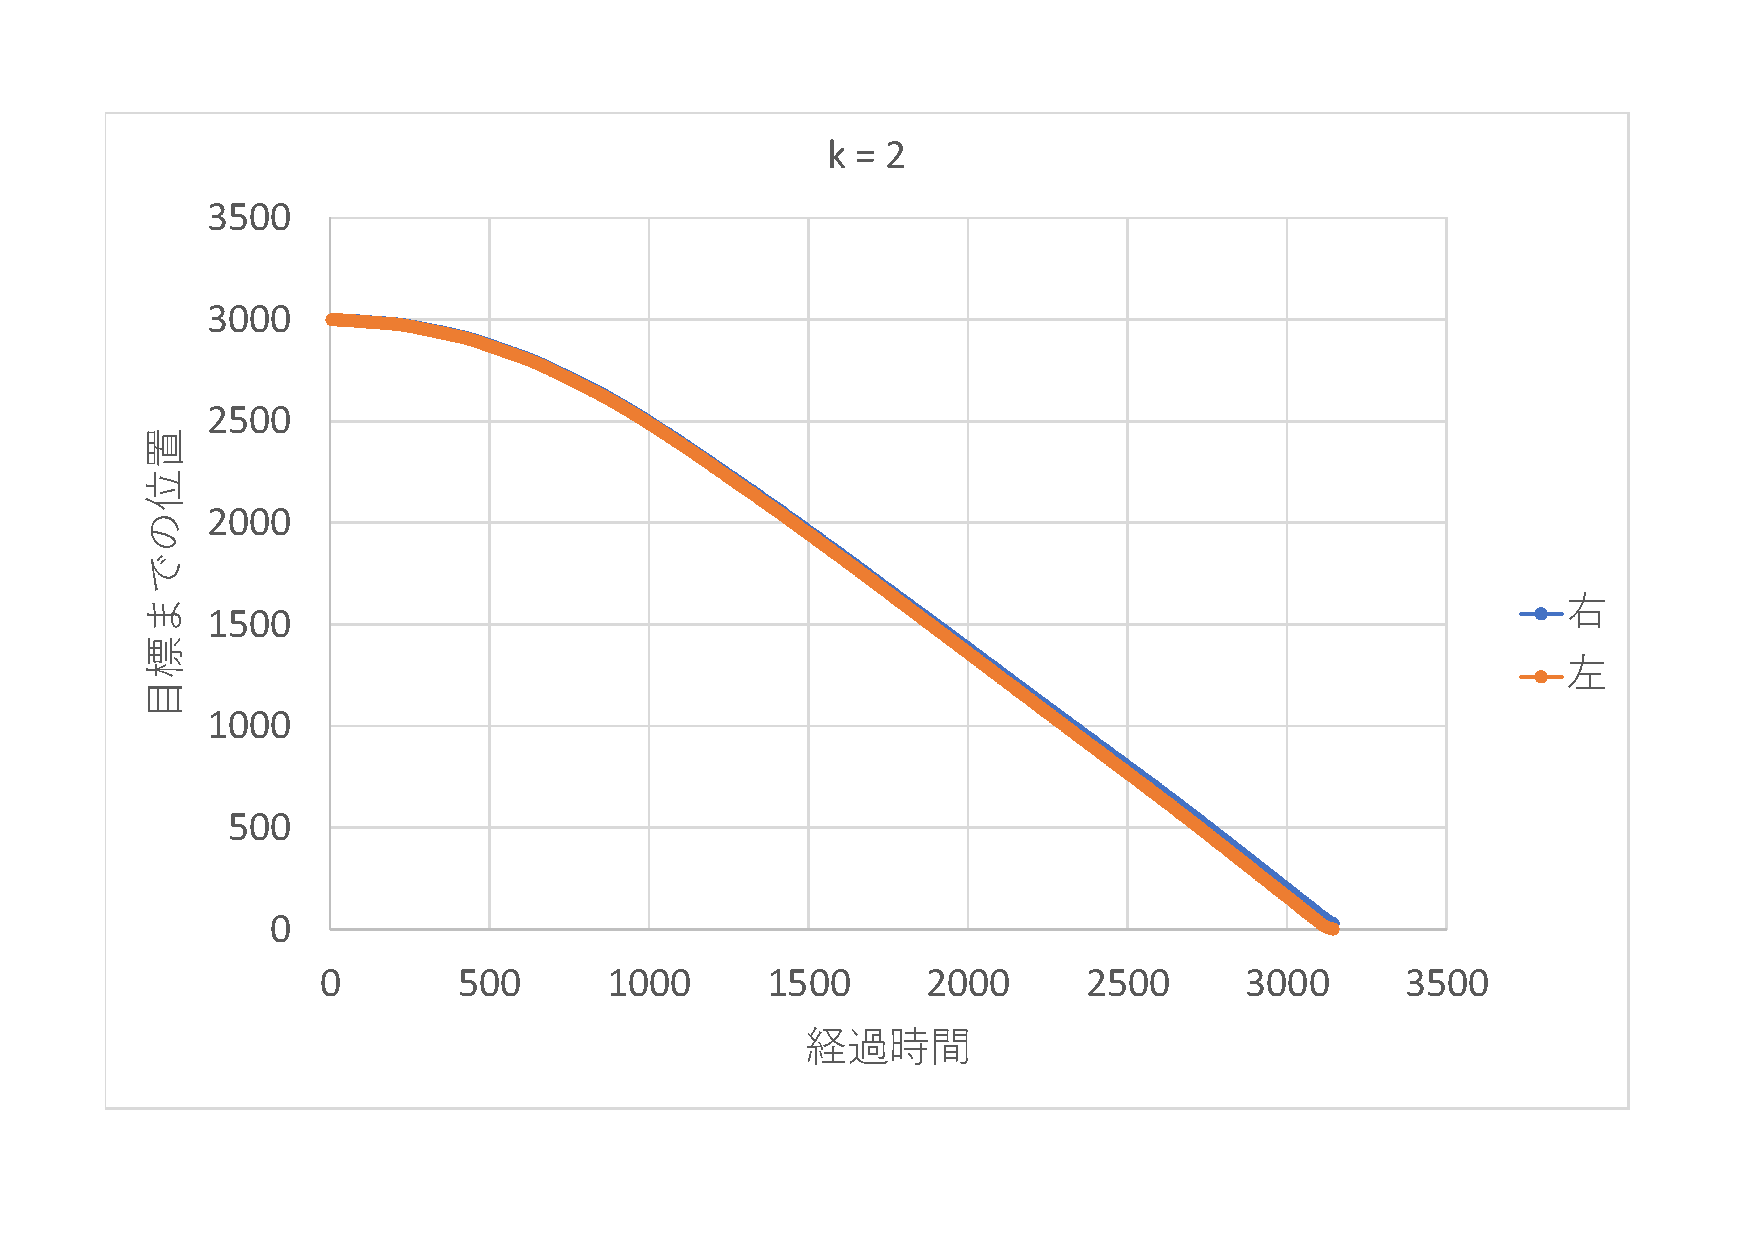
\includegraphics[width=\linewidth]{img/17/17_fuka_K2.pdf}
  \label{im34}
  }
  \subfigure[$k=2$ 負荷無し]{
  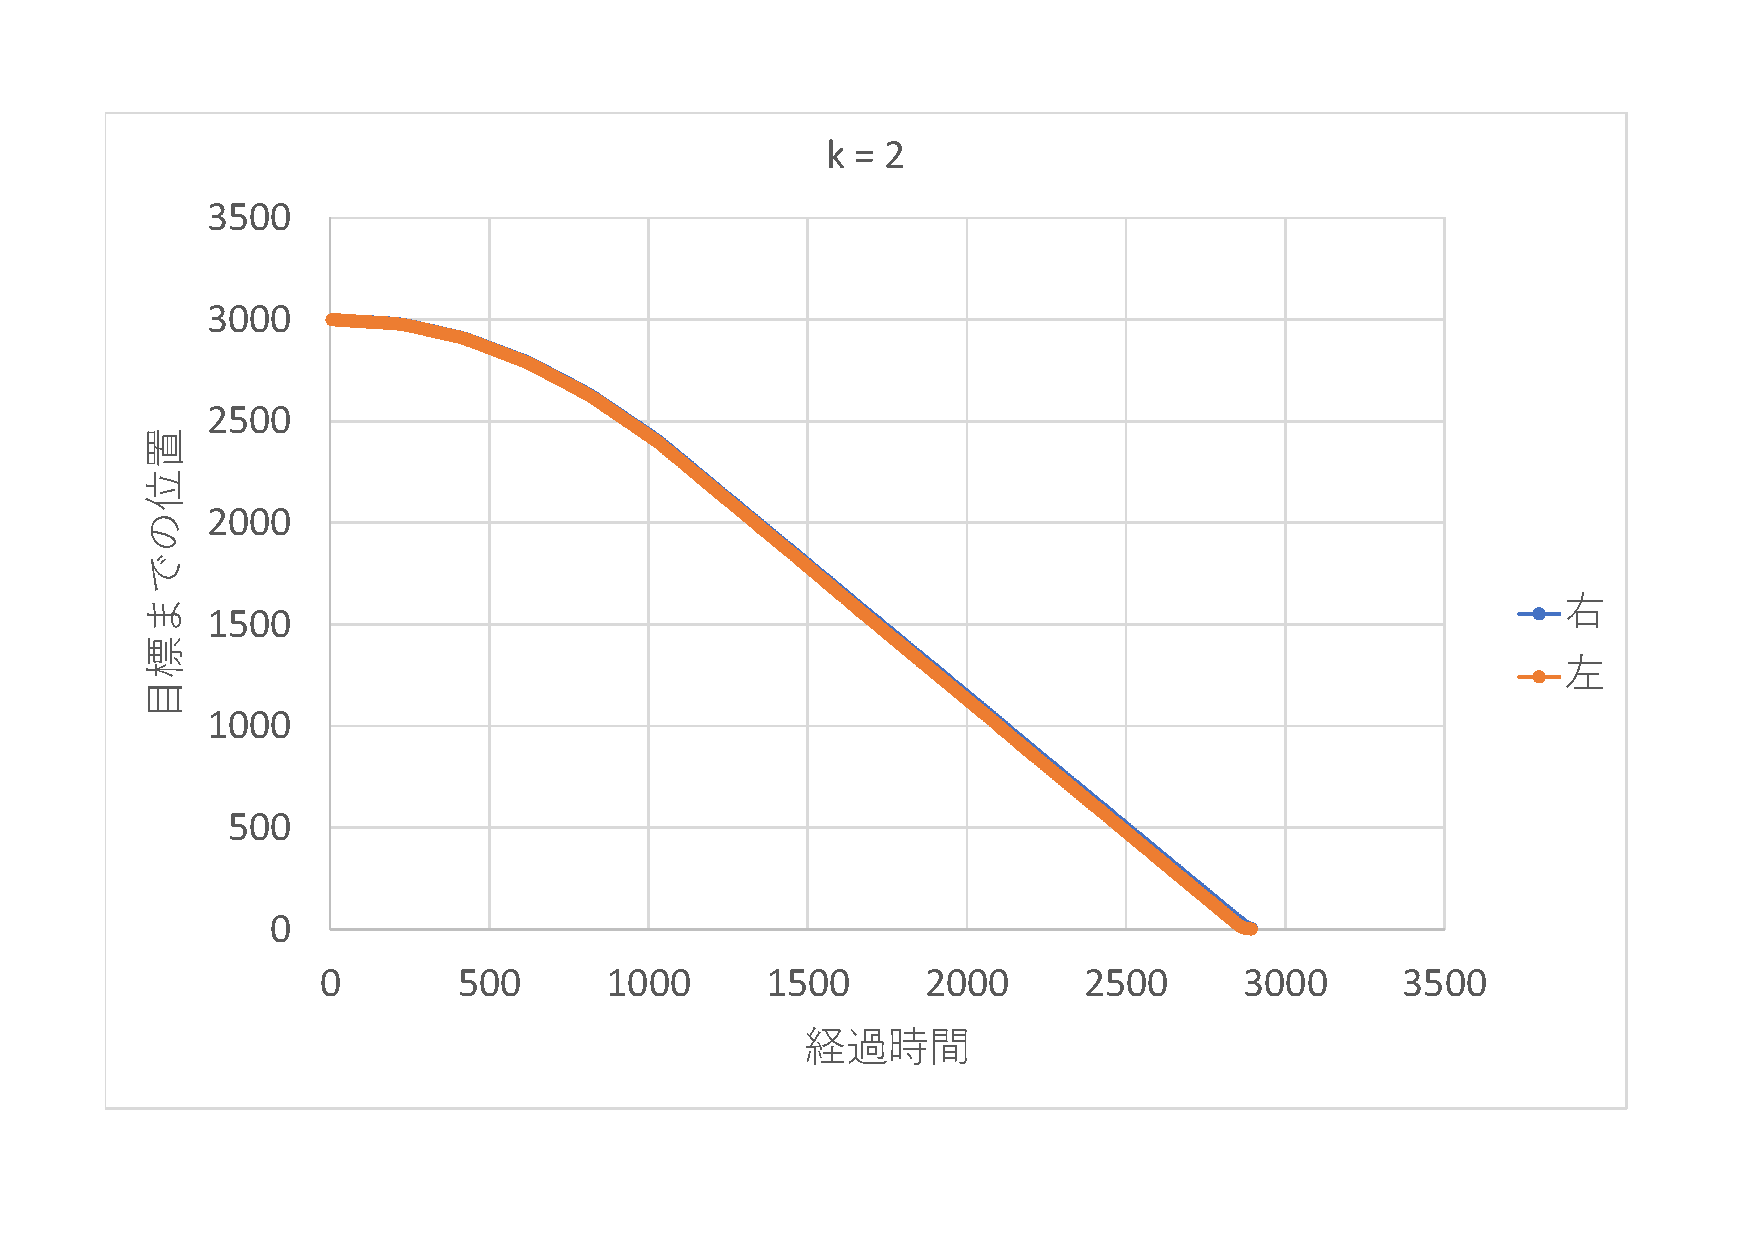
\includegraphics[width=\linewidth]{img/17/17_non_K2.pdf}
  \label{im35}
  }
  \caption{$k=2$のステップ応答}
  \end{center}
\end{figure}

\begin{figure}
  \begin{center}
  \subfigure[$k=3$ 負荷有り]{
  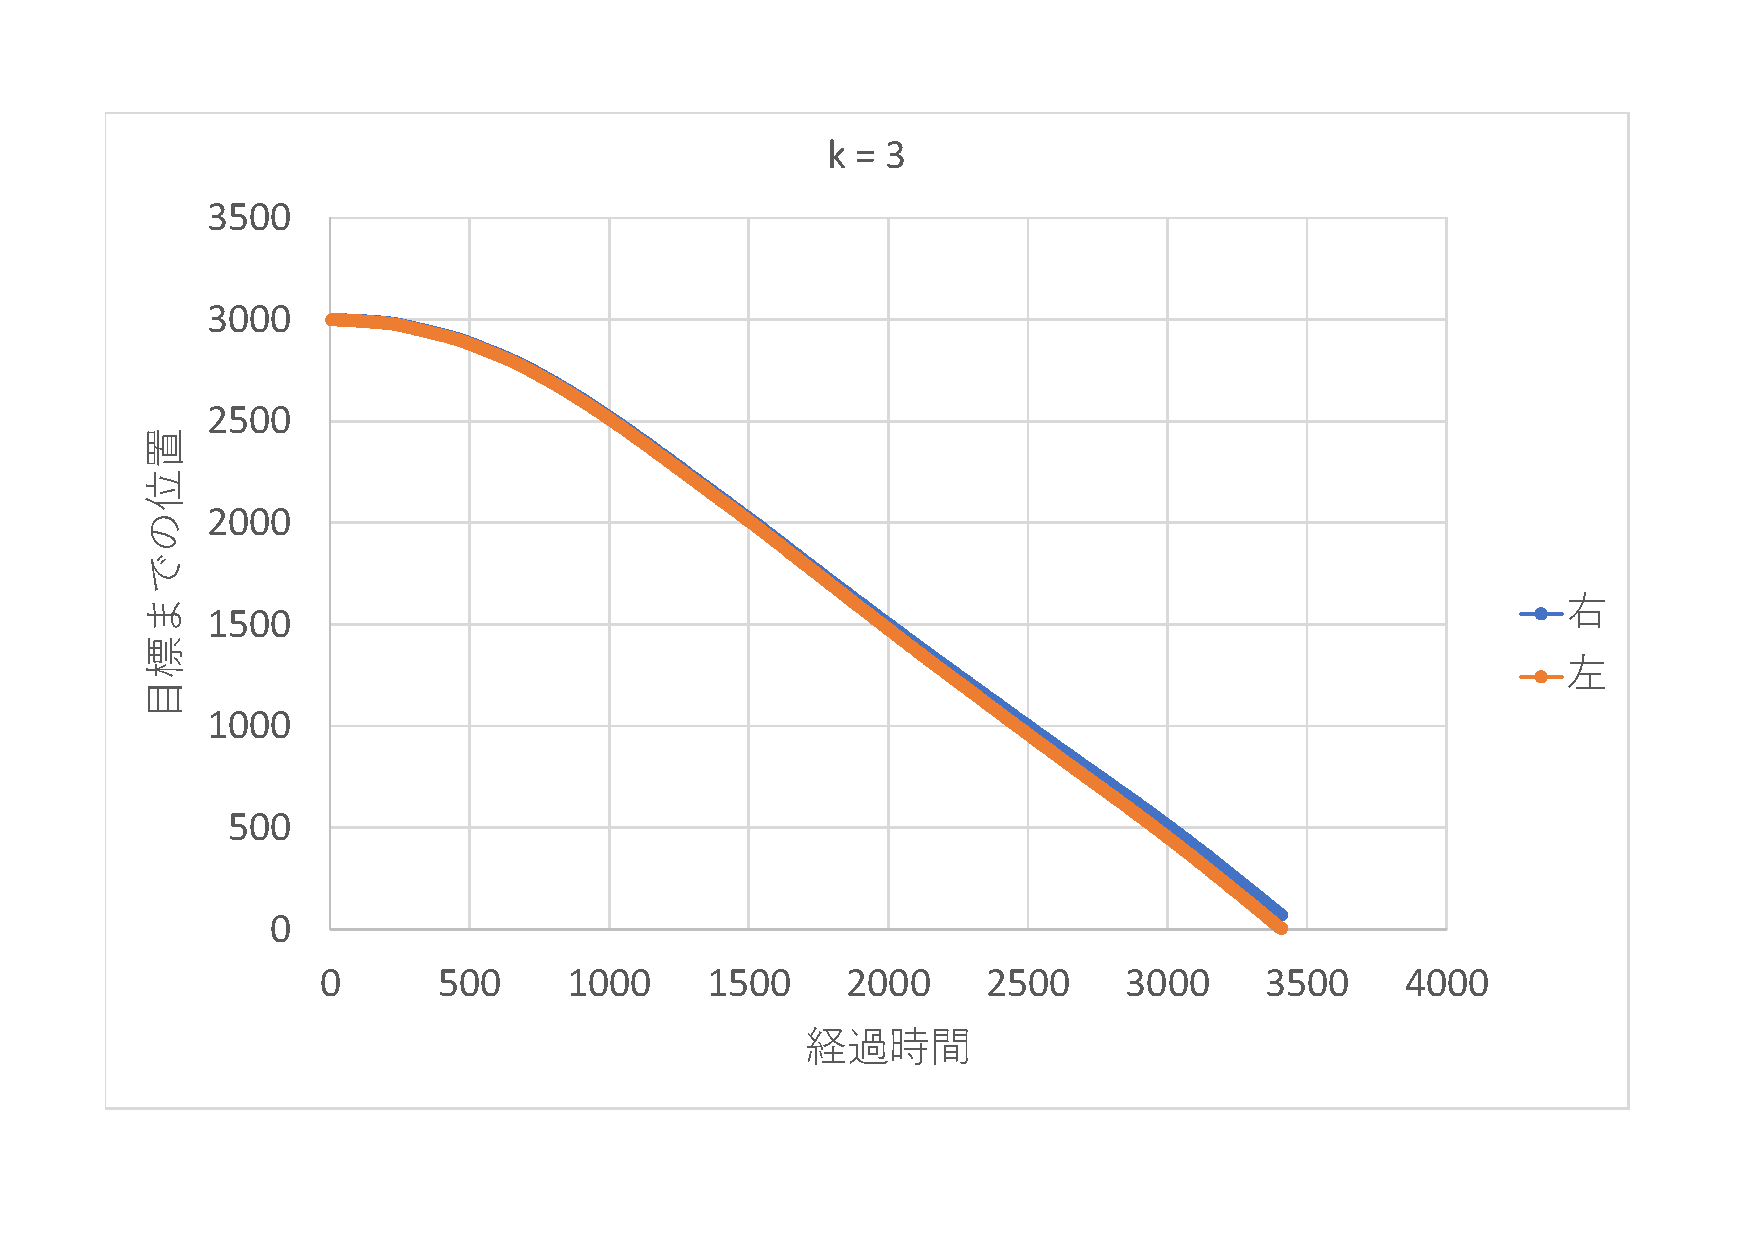
\includegraphics[width=\linewidth]{img/17/17_fuka_K3.pdf}
  \label{im36}
  }
  \subfigure[$k=3$ 負荷無し]{
  \includegraphics[width=\linewidth]{img/17/17_non_K3.pdf}
  \label{im37}
  }
  \caption{$k=3$のステップ応答}
  \end{center}
\end{figure}

\begin{figure}
  \begin{center}
  \subfigure[$k=6$ 負荷有り]{
  \includegraphics[width=\linewidth]{img/17/17_fuka_K6.pdf}
  \label{im38}
  }
  \subfigure[$k=6$ 負荷無し]{
  \includegraphics[width=\linewidth]{img/17/17_non_K6.pdf}
  \label{im39}
  }
  \caption{$k=6$のステップ応答}
  \end{center}
\end{figure}

\begin{figure}
  \begin{center}
  \subfigure[$k=10$ 負荷有り]{
  \includegraphics[width=\linewidth]{img/17/17_fuka_K10.pdf}
  \label{im40}
  }
  \subfigure[$k=10$ 負荷無し]{
  \includegraphics[width=\linewidth]{img/17/17_non_K10.pdf}
  \label{im41}
  }
  \caption{$k=10$のステップ応答}
  \end{center}
\end{figure}

\mysection{演習18}
\subsection{実行プログラム}
実行プログラムをソースコード\ref{s18}に示す。

\begin{lstlisting}[caption=演習18のプログラム,label=s18]
#include <stdio.h>
#include <math.h>
#include <process.h>
#include <dos.h>
#include "v25.h"
#include "ms.h"

#define D2R         (M_PI/180)
#define R2D         (180/M_PI)
#define RADIUS	15.0
#define DISTANCE    34.0
#define REDUCTION   19.225
#define CPR         400
#define MMPS        (60*REDUCTION/(2.0*M_PI*RADIUS))
#define DPC         (2.0*M_PI*RADIUS/((float)CPR*REDUCTION))
#define APC         (DPC/(2*DISTANCE))
#define DMAX        1000
#define THRESH_D    10
#define THRESH_Q    5*D2R
#define THRESH_V    50

#define ABS(x)      (x<0?-(x):(x))

void estimate(double *px,double *py,double *pq,long *pt);
void translate(double d,double vmax,double gain);
void rotate(double qd,double wmax,double gain);

int k=0;
int xi[DMAX],yi[DMAX],qi[DMAX];
long ti[DMAX];

int main(void)
{
    double x,y,q;
    int i;
    int kp=8,ki_inv=8;
    int vmax = 100;
    int wmax = 100/DISTANCE;
    int nl,nr;
    long t,nt;
    FILE *fp;

    ms_init();
    ms_motor_on();
    ms_set_gain(kp,ki_inv);

    estimate(&x,&y,&q,&t);
    rotate(360*D2R,wmax,5);
    translate(1000,vmax,5);

    ms_set_v(0,0);
    do{
        estimate(&x,&y,&q,&t);
        ms_read_v(&nl,&nr,&nt);
    }while(nl != 0 || nr != 0);

    ms_motor_off();

    if((fp=fopen("data.dat","wt"))==NULL)
    {
        printf("Can't open file...\n");
    }

    for(i=0;i<k;i++)
    {
        fprintf(fp,"%5d %5d %5d %5ld\n",xi[i],yi[i],qi[i],ti[i]);
    }
    fclose(fp);
    return 0;
}

void estimate(double *px,double *py,double *pq,long *pt)
{
    static long cl0=0,cr0=0;
    static double x=0.0,y=0.0,q=0.0;
    long cl,cr,ct;
    int dl,dr;
    double ds;

    ms_read_c(&cl,&cr,&ct);
    dl=cl-cl0;
    dr=cr-cr0;
    cl0=cl;
    cr0=cr;
    ds=DPC/2*(dr+dl);
    x += ds*cos(q);
    y += ds*sin(q);
    q += APC*(dr-dl);

    *px=x;
    *py=y;
    *pq=q;
    *pt=ct;
    if (k<DMAX)
    {
        xi[k]=10*x;
        yi[k]=10*y;
        qi[k]=1000*q;
        ti[k]=ct;
        k++;
    }    

}

void translate(double d,double vmax,double gain)
{
    double x0,y0,q0,x,y,q;
    long t0,t,nt;
    double cosq0,sinq0,dd,vc;
    int nc,nl,nr;

    estimate(&x0,&y0,&q0,&t0);
    cosq0=cos(q0);
    sinq0=sin(q0);
    x=x0;
    y=y0;
    q=q0;
    t=t0;

    do
    {
        dd=cosq0*(x-x0)+sinq0*(y-y0);
        vc=gain*(d-dd);
        if (ABS(vc)>vmax)
        {
            vc=(vc<0.0)?-vmax:vmax;
        }
        nc=vc*MMPS;
        ms_set_v(nc,nc);
        estimate(&x,&y,&q,&t);
        ms_read_v(&nl,&nr,&nt);
    } while (ABS(d-dd)>THRESH_D||ABS(nl)>THRESH_V||ABS(nr)>THRESH_V);
}

void rotate(double qd,double wmax,double gain)
{
  double x0,y0,q0,x,y,q;
  long t0,t,nt;
  double qq,wc,v,dw;
  int nl,nr;

  estimate(&x0,&y0,&q0,&t0);
  x=x0;
  y=y0;
  q=q0;
  t=t0;

  do{
  qq=q-q0;
  wc=gain*(qd-qq);
  if(ABS(wc)>wmax)
  {
    wc=(wc<0.0) ? -wmax:wmax;
  }
  dw=DISTANCE*wc;
  nl=-MMPS*dw;
  nr=MMPS*dw;
  ms_set_v(nl,nr);
  estimate(&x,&y,&q,&t);
  ms_read_v(&nl,&nr,&nt);
  }while (ABS(qd-qq)>THRESH_Q||ABS(nl)>THRESH_V||ABS(nr)>THRESH_V);
}
\end{lstlisting}

\mysubsection{実行結果}
ロボットが、その場で360度回転して1000[mm]直進する。
回転角度が360度ちょうどであるが、直進動作時に、
左右のモータの始動に差が生じるため、始動の遅いモータの方に
やや曲がってから直進する現象が生じた。
\mysection{演習19}
\subsection{実行プログラム}
実行プログラムをソースコード\ref{s19}に示す。
パラメータ値は、\textgt{RADIUS}を変化させると、
回転量が変化し、ロボットの回転と進行距離の両方が代わるため、
DISTANCEの値のみを変更した。\textgt{DISTANCE}の実測値を計測し、
DISTANCEの値を上下に変化させて、34.0から34.05に変更した。
360度回転は、指示値通りに動くが、直進の際の始動にモータの左右差が
あったため、それを考慮した上で34.05の値とした。

\begin{lstlisting}[caption=演習19のプログラム,label=s19]
#include <stdio.h>
#include <math.h>
#include <process.h>
#include <dos.h>
#include "v25.h"
#include "ms.h"

#define D2R         (M_PI/180)
#define R2D         (180/M_PI)
#define RADIUS	15.0
#define DISTANCE    34.05
#define REDUCTION   19.225
#define CPR         400
#define MMPS        (60*REDUCTION/(2.0*M_PI*RADIUS))
#define DPC         (2.0*M_PI*RADIUS/((float)CPR*REDUCTION))
#define APC         (DPC/(2*DISTANCE))
#define DMAX        1000
#define THRESH_D    10
#define THRESH_Q    5*D2R
#define THRESH_V    50

#define ABS(x)      (x<0?-(x):(x))

void estimate(double *px,double *py,double *pq,long *pt);
void translate(double d,double vmax,double gain);
void rotate(double qd,double wmax,double gain);

int k=0;
int xi[DMAX],yi[DMAX],qi[DMAX];
long ti[DMAX];

int main(void)
{
    double x,y,q;
    int i;
    int kp=8,ki_inv=8;
    int vmax = 100;
    int wmax = 100/DISTANCE;
    int nl,nr;
    long t,nt;
    FILE *fp;

    ms_init();
    ms_motor_on();
    ms_set_gain(kp,ki_inv);

    estimate(&x,&y,&q,&t);
    rotate(360*D2R,wmax,5);
    translate(1000,vmax,5);

    ms_set_v(0,0);
    do{
        estimate(&x,&y,&q,&t);
        ms_read_v(&nl,&nr,&nt);
    }while(nl != 0 || nr != 0);

    ms_motor_off();

    if((fp=fopen("data.dat","wt"))==NULL)
    {
        printf("Can't open file...\n");
    }

    for(i=0;i<k;i++)
    {
        fprintf(fp,"%5d %5d %5d %5ld\n",xi[i],yi[i],qi[i],ti[i]);
    }
    fclose(fp);
    return 0;
}

void estimate(double *px,double *py,double *pq,long *pt)
{
    static long cl0=0,cr0=0;
    static double x=0.0,y=0.0,q=0.0;
    long cl,cr,ct;
    int dl,dr;
    double ds;

    ms_read_c(&cl,&cr,&ct);
    dl=cl-cl0;
    dr=cr-cr0;
    cl0=cl;
    cr0=cr;
    ds=DPC/2*(dr+dl);
    x += ds*cos(q);
    y += ds*sin(q);
    q += APC*(dr-dl);

    *px=x;
    *py=y;
    *pq=q;
    *pt=ct;
    if (k<DMAX)
    {
        xi[k]=10*x;
        yi[k]=10*y;
        qi[k]=1000*q;
        ti[k]=ct;
        k++;
    }    

}

void translate(double d,double vmax,double gain)
{
    double x0,y0,q0,x,y,q;
    long t0,t,nt;
    double cosq0,sinq0,dd,vc;
    int nc,nl,nr;

    estimate(&x0,&y0,&q0,&t0);
    cosq0=cos(q0);
    sinq0=sin(q0);
    x=x0;
    y=y0;
    q=q0;
    t=t0;

    do
    {
        dd=cosq0*(x-x0)+sinq0*(y-y0);
        vc=gain*(d-dd);
        if (ABS(vc)>vmax)
        {
            vc=(vc<0.0)?-vmax:vmax;
        }
        nc=vc*MMPS;
        ms_set_v(nc,nc);
        estimate(&x,&y,&q,&t);
        ms_read_v(&nl,&nr,&nt);
    } while (ABS(d-dd)>THRESH_D||ABS(nl)>THRESH_V||ABS(nr)>THRESH_V);
}

void rotate(double qd,double wmax,double gain)
{
  double x0,y0,q0,x,y,q;
  long t0,t,nt;
  double qq,wc,v,dw;
  int nl,nr;

  estimate(&x0,&y0,&q0,&t0);
  x=x0;
  y=y0;
  q=q0;
  t=t0;

  do{
  qq=q-q0;
  wc=gain*(qd-qq);
  if(ABS(wc)>wmax)
  {
    wc=(wc<0.0) ? -wmax:wmax;
  }
  dw=DISTANCE*wc;
  nl=-MMPS*dw;
  nr=MMPS*dw;
  ms_set_v(nl,nr);
  estimate(&x,&y,&q,&t);
  ms_read_v(&nl,&nr,&nt);
  }while (ABS(qd-qq)>THRESH_Q||ABS(nl)>THRESH_V||ABS(nr)>THRESH_V);
}
\end{lstlisting}

\mysubsection{実行結果}
ロボットが、その場で360度回転して1000[mm]直進する。
回転角度を360度より浅くして、直進動作時に左右のモータの始動差を吸収して、
360度方向に直進する。

\mysection{演習20}
\subsection{実行プログラム}
実行プログラムをソースコード\ref{s20}に示す。
ロボットの初期位置を$(x_s, y_s, \theta_s) = (0, 0, 0)$としている。

\begin{lstlisting}[caption=演習20のプログラム,label=s20]
#include <stdio.h>
#include <math.h>
#include <process.h>
#include <dos.h>
#include "v25.h"
#include "ms.h"

#define D2R         (M_PI/180)
#define R2D         (180/M_PI)
#define RADIUS	15.0
#define DISTANCE    34.05
#define REDUCTION   19.225
#define CPR         400
#define MMPS        (60*REDUCTION/(2.0*M_PI*RADIUS))
#define DPC         (2.0*M_PI*RADIUS/((float)CPR*REDUCTION))
#define APC         (DPC/(2*DISTANCE))
#define DMAX        1000
#define THRESH_D    10
#define THRESH_Q    5*D2R
#define THRESH_V    50

#define ABS(x)      (x<0?-(x):(x))

void estimate(double *px,double *py,double *pq,long *pt);
void translate(double d,double vmax,double gain);
void rotate(double qd,double wmax,double gain);

int k=0;
int xi[DMAX],yi[DMAX],qi[DMAX];
long ti[DMAX];

int main(void)
{
    double x,y,q;
    double x_d=0,x_s=0,y_d=0,y_s=0,th_s=0,th_d=0,th_1=0,th_2=0,a_0=0;
    int i;
    int kp=8,ki_inv=8;
    int vmax = 100;
    int wmax = 100/DISTANCE;
    int nl,nr;
    long t,nt;
    FILE *fp;




    while(1){
    ms_init();
        ms_motor_on();
        ms_set_gain(kp,ki_inv);
    printf("x_d y_d th_d\n");
    scanf("%lf %lf %lf",&x_d,&y_d,&th_d);
        estimate(&x,&y,&q,&t);
    th_1=atan2(y_d-y_s,x_d-x_s)-th_s;
        rotate(th_1,wmax,5);
    a_0=sqrt((x_d-x_s)*(x_d-x_s)+(y_d-y_s)*(y_d-y_s));
        translate(a_0,vmax,5);
    th_2=th_d*D2R-th_1-th_s;
    rotate(th_2,wmax,5);
    printf("aaa\n");
    x_s=x_d;
    y_s=y_d;
    th_s=th_d;

        ms_set_v(0,0);
        do{
        estimate(&x,&y,&q,&t);
        ms_read_v(&nl,&nr,&nt);
        }while(nl != 0 || nr != 0);

    ms_motor_off();
    }
    return 0;
}

void estimate(double *px,double *py,double *pq,long *pt)
{
    static long cl0=0,cr0=0;
    static double x=0.0,y=0.0,q=0.0;
    long cl,cr,ct;
    int dl,dr;
    double ds;

    ms_read_c(&cl,&cr,&ct);
    dl=cl-cl0;
    dr=cr-cr0;
    cl0=cl;
    cr0=cr;
    ds=DPC/2*(dr+dl);
    x += ds*cos(q);
    y += ds*sin(q);
    q += APC*(dr-dl);

    *px=x;
    *py=y;
    *pq=q;
    *pt=ct;
    if (k<DMAX)
    {
        xi[k]=10*x;
        yi[k]=10*y;
        qi[k]=1000*q;
        ti[k]=ct;
        k++;
    }    

}

void translate(double d,double vmax,double gain)
{
    double x0,y0,q0,x,y,q;
    long t0,t,nt;
    double cosq0,sinq0,dd,vc;
    int nc,nl,nr;

    estimate(&x0,&y0,&q0,&t0);
    cosq0=cos(q0);
    sinq0=sin(q0);
    x=x0;
    y=y0;
    q=q0;
    t=t0;

    do
    {
        dd=cosq0*(x-x0)+sinq0*(y-y0);
        vc=gain*(d-dd);
        if (ABS(vc)>vmax)
        {
            vc=(vc<0.0)?-vmax:vmax;
        }
        nc=vc*MMPS;
        ms_set_v(nc,nc);
        estimate(&x,&y,&q,&t);
        ms_read_v(&nl,&nr,&nt);
    } while (ABS(d-dd)>THRESH_D||ABS(nl)>THRESH_V||ABS(nr)>THRESH_V);
}

void rotate(double qd,double wmax,double gain)
{
    double x0,y0,q0,x,y,q;
    long t0,t,nt;
    double qq,wc,v,dw;
    int nl,nr;

    estimate(&x0,&y0,&q0,&t0);
    x=x0;
    y=y0;
    q=q0;
    t=t0;

    do{
    qq=q-q0;
    wc=gain*(qd-qq);
    if(ABS(wc)>wmax)
    {
        wc=(wc<0.0) ? -wmax:wmax;
    }
    dw=DISTANCE*wc;
    nl=-MMPS*dw;
    nr=MMPS*dw;
    ms_set_v(nl,nr);
    estimate(&x,&y,&q,&t);
    ms_read_v(&nl,&nr,&nt);
    printf("%lf %lf %lf\n", ABS(qd-qq), ABS(nl), ABS(nr));
    }while (ABS(qd-qq)>THRESH_Q||ABS(nl)>THRESH_V||ABS(nr)>THRESH_V);
}
\end{lstlisting}

\mysubsection{実行結果}
目標位置$(x_d, y_d, \theta_d)$を入力すると、
目標方向を向き、目標の座標$(x_d, y_d)$の方向に直進し、
到着すると$\theta_d$方向に向きを変える。
目標位置・姿勢の状態をとると、初期値を現在値に更新し、
再び目標位置の入力待機を行う。その後、目標位置の入力と移動の処理を繰り返して行うことができる。
その際、目標位置の入力前にモータの電圧をオンと初期化、出力後にモータの電圧をオフ
を毎ループごとに繰り返し行う。

\mysection{演習21}
\subsection{実行プログラム}
実行プログラムをソースコード\ref{s21}に示す。

\begin{lstlisting}[caption=演習21のプログラム,label=s21]
#include <stdio.h>
#include <math.h>
#include <process.h>
#include <dos.h>
#include "v25.h"
#include "ms.h"

#define D2R         (M_PI/180)
#define R2D         (180/M_PI)
#define RADIUS	15.0
#define DISTANCE    34.05
#define REDUCTION   19.225
#define CPR         400
#define MMPS        (60*REDUCTION/(2.0*M_PI*RADIUS))
#define DPC         (2.0*M_PI*RADIUS/((float)CPR*REDUCTION))
#define APC         (DPC/(2*DISTANCE))
#define DMAX        1000
#define THRESH_D    10
#define THRESH_Q    5*D2R
#define THRESH_V    1

#define GOALX       1200
#define GOALY       1000
#define GOALQ       0
#define VMAX        150
#define WMAX        (VMAX/(3*DISTANCE))
#define REVERSE     200

#define ABS(x)      (x<0?-(x):(x))

void estimate(double *px,double *py,double *pq,long *pt);
void translate(double d,double vmax,double gain);
int translate2(double d,double vmax,double gain);
void rotate(double qd,double wmax,double gain);
double seikika(double angle);
void avoid(int j);

int k=0;
int xi[DMAX],yi[DMAX],qi[DMAX];
long ti[DMAX];

int main(void)
{
    double x,y,q,q1,q2,dl,dq;
    int i,j;
    int kp=8,ki_inv=8;
    int nl,nr;
    long t,nt;
    FILE *fp;

    ms_init();
    ms_set_gain(kp,ki_inv);
    ms_motor_on();
    ms_wait(1000);

    while (1)
    {
        estimate(&x,&y,&q,&t);

        dl=sqrt((GOALX-x)*(GOALX-x)+(GOALY-y)*(GOALY-y));
        if(dl<THRESH_D) break;

        dq=atan2(GOALY-y,GOALX-x)-q;
        dq=seikika(dq);
        rotate(dq,WMAX,5);

        j=translate2(dl,VMAX,5);

        avoid(j);
    }

    while (1)
    {
        estimate(&x,&y,&q,&t);

        dq=seikika(GOALQ-q);
        if (ABS(dq)<THRESH_Q)   break;

        rotate(dq,WMAX,5);
    }

      ms_motor_off();

    if((fp=fopen("data.dat","wt"))==NULL)
    {
        printf("Can't open file...\n");
        exit(1);
    }

    for(i=0;i<k;i++)
    {
        fprintf(fp,"%5d %5d %5d %5ld\n",xi[i],yi[i],qi[i],ti[i]);
    }
    fclose(fp);
    return 0;
}

void estimate(double *px,double *py,double *pq,long *pt)
{
    static long cl0=0,cr0=0;
    static double x=0.0,y=0.0,q=0.0;
    long cl,cr,ct;
    int dl,dr;
    double ds;

    ms_read_c(&cl,&cr,&ct);
    dl=cl-cl0;
    dr=cr-cr0;
    cl0=cl;
    cr0=cr;
    ds=DPC/2*(dr+dl);
    x += ds*cos(q);
    y += ds*sin(q);
    q += APC*(dr-dl);

    *px=x;
    *py=y;
    *pq=q;
    *pt=ct;
    if (k<DMAX)
    {
        xi[k]=10*x;
        yi[k]=10*y;
        qi[k]=1000*q;
        ti[k]=ct;
        k++;
    }    

}

void translate(double d,double vmax,double gain)
{
    double x0,y0,q0,x,y,q;
    long t0,t,nt;
    double cosq0,sinq0,dd,vc;
    int nc,nl,nr;

    estimate(&x0,&y0,&q0,&t0);
    cosq0=cos(q0);
    sinq0=sin(q0);
    x=x0;
    y=y0;
    q=q0;
    t=t0;

    do
    {
        dd=cosq0*(x-x0)+sinq0*(y-y0);
        vc=gain*(d-dd);
        if (ABS(vc)>vmax)
        {
            vc=(vc<0.0)?-vmax:vmax;
        }
        nc=vc*MMPS;
        ms_set_v(nc,nc);
        estimate(&x,&y,&q,&t);
        ms_read_v(&nl,&nr,&nt);
    } while (ABS(d-dd)>THRESH_D||ABS(nl)>THRESH_V||ABS(nr)>THRESH_V);
}

int translate2(double d,double vmax,double gain)
{
    double x0,y0,q0,x,y,q,g;
    long t0,t,nt;
    double cosq0,sinq0,dd,vc;
    int nc,nl,nr,s[3],check;

    estimate(&x0,&y0,&q0,&t0);
    cosq0=cos(q0);
    sinq0=sin(q0);
    x=x0;
    y=y0;
    q=q0;
    t=t0;

    do
    {
        ms_ifr(s);
        check = 1*s[0]+2*s[1]+4*s[2];
        ms_read_v(&nl,&nr,&nt);

        if (check)
        {
            for (g = 1; g > 0; g-=0.01)
                ms_set_v((int)(nl*g),(int)(nr*g));
            
            return check;   
        }
        
        dd=cosq0*(x-x0)+sinq0*(y-y0);

        vc=gain*(d-dd);

        if (ABS(vc)>vmax)
        {
            vc = (vc < 0.0) ? -vmax : vmax;
        }
        nc=vc*MMPS;
        ms_set_v(nc,nc);
        estimate(&x,&y,&q,&t);
        ms_read_v(&nl,&nr,&nt);
    } while (ABS(d-dd)>THRESH_D||ABS(nl)>THRESH_V||ABS(nr)>THRESH_V);
    return 0;
}

void rotate(double qd,double wmax,double gain)
{
  double x0,y0,q0,x,y,q;
  long t0,t,nt;
  double qq,wc,v,dw;
  int nl,nr;

  estimate(&x0,&y0,&q0,&t0);
  x=x0;
  y=y0;
  q=q0;
  t=t0;

  do{
  qq=q-q0;
  wc=gain*(qd-qq);
  if(ABS(wc)>wmax)
  {
    wc=(wc<0.0) ? -wmax:wmax;
  }
  dw=DISTANCE*wc;
  nl=-MMPS*dw;
  nr=MMPS*dw;
  ms_set_v(nl,nr);
  estimate(&x,&y,&q,&t);
  ms_read_v(&nl,&nr,&nt);
  }while (ABS(qd-qq)>THRESH_Q||ABS(nl)>THRESH_V||ABS(nr)>THRESH_V);
}

double seikika(double angle)
{
    while(angle>M_PI)   angle -= 2*M_PI;
    while(angle<=-M_PI)   angle += 2*M_PI;
    return angle;
}

void avoid(int j)
{
    if(j!=0)
    {
        translate(-REVERSE,VMAX,5);
        if(j&1) rotate(-60*D2R,WMAX,5);
        else rotate(60*D2R,WMAX,5);
        translate(REVERSE,VMAX,5);
    }
}
\end{lstlisting}

\mysubsection{実行結果}
ロボットを起動させると、前進し、近接センサが障害物に反応すると、
ロボットは後退し、一旦後退する。その後センサ値が1であれば60度右に旋回し、
それ以外ならば、左に60度旋回する。その後、前方に進む。


\mysection{演習22}
\subsection{実行プログラム}
実行プログラムをソースコード\ref{s22}に示す。
本プログラムは、移動平均法を用いて、近接センサの値を平均化し、
標本化している。過去5つのセンサデータ(0か1)を保持し、その平均値が0.8
以上なら障害物を検知した場合の処理を行う。

\begin{lstlisting}[caption=演習22のプログラム,label=s22]
#include <stdio.h>
#include <math.h>
#include <process.h>
#include <dos.h>
#include "v25.h"
#include "ms.h"

#define D2R         (M_PI/180)
#define R2D         (180/M_PI)
#define RADIUS	15.0
#define DISTANCE    34.05
#define REDUCTION   19.225
#define CPR         400
#define MMPS        (60*REDUCTION/(2.0*M_PI*RADIUS))
#define DPC         (2.0*M_PI*RADIUS/((float)CPR*REDUCTION))
#define APC         (DPC/(2*DISTANCE))
#define DMAX        1000
#define THRESH_D    10
#define THRESH_Q    5*D2R
#define THRESH_V    1

#define GOALX       1200
#define GOALY       1000
#define GOALQ       0
#define VMAX        150
#define WMAX        (VMAX/(3*DISTANCE))
#define REVERSE     200

#define ABS(x)      (x<0?-(x):(x))

#define WIDTH 10    /*センサのデータを保存する個数*/

void estimate(double *px,double *py,double *pq,long *pt);
void translate(double d,double vmax,double gain);
int translate2(double d,double vmax,double gain);
void rotate(double qd,double wmax,double gain);
double seikika(double angle);
void avoid(int j);

int k=0;
int xi[DMAX],yi[DMAX],qi[DMAX];
long ti[DMAX];

    int sum_s [3]={0,0,0};   /*直近10個のデータの合計    0:左,1:中央,2:右(bs)*/
    int bp=0;   /*最新データの場所*/
    int data_s[3][WIDTH];  /*直近10個のデータ (buff)*/

int main(void)
{
    double x,y,q,q1,q2,dl,dq;
    int i,j;
    int kp=8,ki_inv=8;
    int nl,nr;
    long t,nt;
    FILE *fp;

    ms_init();
    ms_set_gain(kp,ki_inv);
    ms_motor_on();
    ms_wait(1000);

    while (1)
    {
        estimate(&x,&y,&q,&t);

        dl=sqrt((GOALX-x)*(GOALX-x)+(GOALY-y)*(GOALY-y));
        if(dl<THRESH_D) break;

        dq=atan2(GOALY-y,GOALX-x)-q;
        dq=seikika(dq);
        rotate(dq,WMAX,5);

        j=translate2(dl,VMAX,5);

        avoid(j);
    }

    while (1)
    {
        estimate(&x,&y,&q,&t);

        dq=seikika(GOALQ-q);
        if (ABS(dq)<THRESH_Q)   break;

        rotate(dq,WMAX,5);
    }

      ms_motor_off();

    if((fp=fopen("data.dat","wt"))==NULL)
    {
        printf("Can't open file...\n");
        exit(1);
    }

    for(i=0;i<k;i++)
    {
        fprintf(fp,"%5d %5d %5d %5ld\n",xi[i],yi[i],qi[i],ti[i]);
    }
    fclose(fp);
    return 0;
}

void estimate(double *px,double *py,double *pq,long *pt)
{
    static long cl0=0,cr0=0;
    static double x=0.0,y=0.0,q=0.0;
    long cl,cr,ct;
    int dl,dr;
    double ds;

    ms_read_c(&cl,&cr,&ct);
    dl=cl-cl0;
    dr=cr-cr0;
    cl0=cl;
    cr0=cr;
    ds=DPC/2*(dr+dl);
    x += ds*cos(q);
    y += ds*sin(q);
    q += APC*(dr-dl);

    *px=x;
    *py=y;
    *pq=q;
    *pt=ct;
    if (k<DMAX)
    {
        xi[k]=10*x;
        yi[k]=10*y;
        qi[k]=1000*q;
        ti[k]=ct;
        k++;
    }    

}

void translate(double d,double vmax,double gain)
{
    double x0,y0,q0,x,y,q;
    long t0,t,nt;
    double cosq0,sinq0,dd,vc;
    int nc,nl,nr;

    estimate(&x0,&y0,&q0,&t0);
    cosq0=cos(q0);
    sinq0=sin(q0);
    x=x0;
    y=y0;
    q=q0;
    t=t0;

    do
    {
        dd=cosq0*(x-x0)+sinq0*(y-y0);
        vc=gain*(d-dd);
        if (ABS(vc)>vmax)
        {
            vc=(vc<0.0)?-vmax:vmax;
        }
        nc=vc*MMPS;
        ms_set_v(nc,nc);
        estimate(&x,&y,&q,&t);
        ms_read_v(&nl,&nr,&nt);
    } while (ABS(d-dd)>THRESH_D||ABS(nl)>THRESH_V||ABS(nr)>THRESH_V);
}

int translate2(double d,double vmax,double gain)
{
    double x0,y0,q0,x,y,q,g;
    long t0,t,nt;
    double cosq0,sinq0,dd,vc;
    int nc,nl,nr,s[3],check;

    int i=0;    /*センサ左中右切り替え用*/

    estimate(&x0,&y0,&q0,&t0);
    cosq0=cos(q0);
    sinq0=sin(q0);
    x=x0;
    y=y0;
    q=q0;
    t=t0;

    do
    {
        ms_ifr(s);

        /*過去WIDTH個のデータの平均でs[i]を判断*/
        for(i=0;i<3;i++)
        {
            // WIDTH 個のデータを捨てるために合計から引く
            sum_s[i] = sum_s[i] - data_s[i][bp] ;

            data_s[i][bp] = s[i] ;      // 最新データを保存

            sum_s[i] = sum_s[i] + s[i] ;         // 最新のデータで合計
            
            // 直近のデータを覚える場所を移動
            bp++ ;
            if ( bp >= WIDTH )
            {
                bp = 0 ;
            }
            
            // 直近wIdth個のデータ割る個数で出した平均が1以上の場合にsを1、1未満の場合sを0とする
            if((sum_s[i]/WIDTH)>=0.8)
            {
                s[i]=1;
            }else{
                s[i]=0;
            }
        }

        check = 1*s[0]+2*s[1]+4*s[2];
        ms_read_v(&nl,&nr,&nt);

        if (check)
        {
            for (g = 1; g > 0; g-=0.01)
                ms_set_v((int)(nl*g),(int)(nr*g));
            
            return check;   
        }
        
        dd=cosq0*(x-x0)+sinq0*(y-y0);

        vc=gain*(d-dd);

        if (ABS(vc)>vmax)
        {
            vc = (vc < 0.0) ? -vmax : vmax;
        }
        nc=vc*MMPS;
        ms_set_v(nc,nc);
        estimate(&x,&y,&q,&t);
        ms_read_v(&nl,&nr,&nt);
    } while (ABS(d-dd)>THRESH_D||ABS(nl)>THRESH_V||ABS(nr)>THRESH_V);
    return 0;
}

void rotate(double qd,double wmax,double gain)
{
  double x0,y0,q0,x,y,q;
  long t0,t,nt;
  double qq,wc,v,dw;
  int nl,nr;

  estimate(&x0,&y0,&q0,&t0);
  x=x0;
  y=y0;
  q=q0;
  t=t0;

  do{
  qq=q-q0;
  wc=gain*(qd-qq);
  if(ABS(wc)>wmax)
  {
    wc=(wc<0.0) ? -wmax:wmax;
  }
  dw=DISTANCE*wc;
  nl=-MMPS*dw;
  nr=MMPS*dw;
  ms_set_v(nl,nr);
  estimate(&x,&y,&q,&t);
  ms_read_v(&nl,&nr,&nt);
  }while (ABS(qd-qq)>THRESH_Q||ABS(nl)>THRESH_V||ABS(nr)>THRESH_V);
}

double seikika(double angle)
{
    while(angle>M_PI)   angle -= 2*M_PI;
    while(angle<=-M_PI)   angle += 2*M_PI;
    return angle;
}

void avoid(int j)
{
    if(j!=0)
    {
        translate(-REVERSE,VMAX,5);
        if(j&1) rotate(-60*D2R,WMAX,5);
        else rotate(60*D2R,WMAX,5);
        translate(REVERSE,VMAX,5);
    }
} 
\end{lstlisting}

\mysubsection{実行結果}
元々センサの入力が高感度であったため、障害物の検知が不安定であった。
しかし、センサの値が平均化することによってそのようなノイズが減り、
障害物検知が安定した。

\end{document}